\documentclass[12pt, letterpaper]{article}
 
 
%==============Packages & Commands=================
\usepackage{graphicx} % Graphics
\usepackage{indentfirst} % Tells LaTeX to indent every paragraph 
\usepackage{setspace} % To set line spacing
\usepackage[longnamesfirst]{natbib} % For references
\usepackage{booktabs} % For tables
\usepackage{rotating} % For sideways tables/figures
\usepackage{amsmath} % Some math symbols
\usepackage[margin = .8in]{geometry}
\usepackage{subcaption}
\usepackage{mdwlist}
\usepackage{pifont}
\usepackage{url}
\usepackage{verbatim}
\usepackage{lscape}
\usepackage[hang,flushmargin]{footmisc} 
%\usepackage{textcomp}
\urlstyle{same}
%\usepackage{appendix}
\usepackage{multirow}
\usepackage[nolists]{endfloat} % Figures and tables at the end
\usepackage{cleveref}
%\usepackage{endnotes}
%/Users/meganstewart/Documents/YML, Sanctuary Documents/JCR Submission 3/Style files/subcaption.sty\let\footnote=\endnote
\graphicspath{{Figures/}}

\usepackage{sectsty}
\sectionfont{\large}
\subsectionfont{\normalsize}

\newcommand{\R}{\texttt{R}\space} % Write R in typewriter font
\newcommand{\trans}[1]{{#1}^{\ensuremath{\mathsf{T}}}} % Transpose symbol 
\bibpunct{(}{)}{;}{a}{}{,} % Reference punctuation 
\usepackage[capposition=top]{floatrow}
\usepackage[flushleft]{threeparttable}

\DeclareDelayedFloatFlavor{sidewaystable}{table} %Allows endfloat to handle sidewaystable
\DeclareDelayedFloatFlavor{sidewaysfigure}{figure} %Allows endfloat to handle sidewaysfigure

%These packages for inserting blue hyperlinks in text (and for linking in-text references to references section)
\usepackage{hyperref}
\usepackage[usenames,dvipsnames,svgnames,table]{xcolor}
\hypersetup{colorlinks=true,
linkcolor=MidnightBlue,
citecolor=MidnightBlue,
filecolor=MidnightBlue,
urlcolor=MidnightBlue}
 % Link colors

%\usepackage{colortbl}
%\definecolor{Gray}{gray}{0.9}
%\pagestyle{empty}

\usepackage{bibentry}

%===============Some new commands==================
\newcommand{\fnote}[1]{\footnote{\begin{doublespace}\normalsize{#1}\vspace{-26pt}\end{doublespace}}} % 12 pt, double spaced footnotes 
\renewcommand{\figureplace}{ % This places [Insert Table X here] and [Insert Figure Y here] in the text
\begin{center}
[Insert \figurename~\thepostfig\ here]
\end{center}}
\renewcommand{\tableplace}{%
\begin{center}
[Insert \tablename~\theposttbl\ here]
\end{center}}



\title{Civil War as State-Making: \\ Strategic Governance in Civil War}
\author{Megan A. Stewart\thanks{Corresponding author. I thank Daniel Byman, Desha Girod, Daniel Nexon, Stathis Kalyvas, Joseph Young, Boaz Atzili, Dave Ohls, Prakhar Sharma, Jake Anderson, Laila Wahedi, Haillie Lee, Paula Ganga, Karin Kitchens, Mark Hines, Eric Mosinger, Therese Anders, David Brenner, Stella Peisch, Alexandra Ma, Elvia Pena Cruz, Micol Bez, Soumyajit Mazumder, Reno Varghese and seminar participants at Yale University, Georgetown University, American University.}\\mas7an@virginia.edu\\\normalsize{Assistant Professor, School of International Service, American University}\\ \normalsize{Post-Doctoral Research Associate, Department of Politics, University of Virginia}}%\affil{School of International Service, American University and Department of Politics, University of Virginia}
\date{}

%===================Startup========================
\begin{document} 
\maketitle
\doublespacing
\vspace{.3in}
\begin{center}
\noindent\textbf{Word Count: 7988 (without abstract)}
\end{center}
\begin{singlespace}
\begin{abstract}
\begin{normalsize}
\noindent Why do some rebel groups provide governance inclusively while most others do not? Some insurgencies divert critical financial and personnel resources to provide benefits to anyone, including non-supporters (e.g. Karen National Union, Eritrean People's Liberation Front). Other groups offer no services or limit their service provision to only those people who support, or are likely to support, the insurgency. The existing literature examines how insurgencies incentivize recruitment by offering selective social services, yet no research addresses why insurgencies provide goods inclusively. I argue that inclusive provision of services legitimates insurgents' claim of sovereignty to domestic and international audiences, and thus is a strategic tool secessionist rebels use to achieve their long-term goal of independence. With new and original data, I use a large-n analysis to test this hypothesis. The results of the analysis support the hypothesis, underscoring the importance insurgent non-violent behavior and addressing key issues such as sovereignty and governance.
\end{normalsize}
\end{abstract}

\begin{quote}
\textbf{Keywords}: Insurgency, civil war, public goods, sovereignty, statehood, secessionist movements, conflict dynamics
\end{quote}
\end{singlespace}
%\thispagestyle{empty}
%\vspace{.3in}
%===================Abstract======================= 
%\newpage
%\thispagestyle{empty}


%================Begin Manuscript==================
%\newpage

%The objective of this chapter is to test the theory that secessionist movements that control territory are more likely to provide public goods than other groups. Territory-controlling secessionist movements are more likely to provide public goods because territorial control makes them competitors of the state they are fighting. Because secessionist movements ultimately seek to be recognized domestically and internationally as the legitimate sovereign of a territorial space, they provide public goods to demonstrate their capacity for being a state. 

%The chapter proceeds as follows. First, I introduce, contextualize and describe the coding procedures for a new, original dataset, the ``Insurgent Social Services Data.'' I then provide some basic descriptive statistics about the variables I have collected, and describe some key trends. In the third section, I introduce the construction of dependent variables, as well as the operationalization of several key covariates used in my model. The next section provides the results for a series of robustness checks, to ensure that the statistical results are strong, before concluding the chapter. The statistical analysis supports my theory, and is robust to several alternative specifications. Taken together, these results show strong support for my theory that secessionist movements that control territory are more likely to provide public goods. 

%\section*{Insurgent Social Services Data}


%In the sections that follow, I describe the variables included in the dataset and how I coded the data. First I describe the different populations of recipients, then I clarify my concepts and coding guidelines for ``provision,'' ``education,'' and ``healthcare.''

%\subsection*{Population of Recipients}

%As noted in the theory chapter, the current research on insurgent social service provision tends to aggregate all types of service provision and fails to distinguish between which populations might benefit from an insurgent's services (Mampilly 2011, Weinstein 2006). Yet disaggregating both the type of services an insurgency offers and the population that the insurgency provides to is a critical distinction.\footnote{Berman and Laitin (2008) make this critical analytic step and focus on insurgent club goods provision. They generate and test a distinct set of hypotheses for insurgent \textit{club goods} provision, but do not focus on \textit{public goods}. In the economics literature, public goods are considered goods that are non-rivalrous (meaning that provision of services to one person will not diminish the services to another) and non-excludable, meaning that anyone can benefit. Club goods on the other hand, are services that are non-rivalrous, but are only provided to a specific group of people.} %As a result, these authors may use dissimilar phenomenon as a point of comparison across cases in a way that could considerably impact their arguments. 

%For example, Weinstein \citeyearpar{weinstein2006inside} argues that insurgencies provide social services as a way to recruit highly committed soldiers who are less opportunistic and thus less likely to commit indiscriminate violence against civilians. More opportunistic recruits likely to commit mass civilian violence may join an insurgency to take advantage of lootable resources or other economic benefits. Weinstein's   argument, however, assumes that social services are provided publicly or to a broad population. If an insurgency only offered education or healthcare to its members, an opportunistic recruit may join an insurgency to receive education or healthcare. In this case, an opportunistic who is more likely to commit violence joined the insurgency in order to receive education. As an example, some combatants  of the Revolutionary United Front fighters in Sierra Leone claimed to have joined the RUF for the purposes of attending their ``bush schools,'' and were also notorious for committing mass violence.\footnote{Peters, Krijn. ``Re-examining voluntarism. Youth combatants in Sierra Leone.'' \textit{Institute for Security Studies Monographs} 100 (2004): 1-35. and Humphreys, Macartan, and Jeremy M. Weinstein. ``Who fights? The determinants of participation in civil war.'' \textit{American Journal of Political Science} 52.2 (2008): 436-455.}



%These data are highly sensitive to the possibility of false positives, most likely to arise in two ways. First, an insurgency may provide services to anyone within a town or territory it controlled, but it would only provide services after expelling or killing anyone unlikely to support the insurgency. The National Liberation Front of Vietnam\footnote{Pike, Douglas. Viet Cong; the Organization and Techniques of the National Liberation Front of South Vietnam. Cambridge, MA: M.I.T., 1966. Print, pgs. 20-1 and 278-9 and Pike, Douglas. The Viet-Cong Strategy of Terror. Cambridge, MA: M.I.T., 1970. Print.} as well as UNITA in Angola were notorious for engaging in these activities.\footnote{Collelo, Thomas. Angola: A Country Study: Research Completed February 1989. Washington, D.C.: U.S. Government Printing Office, 1991, pg.s. 103-109. URL: http://www.dtic.mil/dtic/tr/fulltext/u2/a234415.pd}

%Second, these data address potential false positives caused by the movement of civilians in wartime to refugee camps. After the start of the civil war, civilians may flee their homes and migrate to refugee camps. Civilians may have the opportunity to choose which camp to go to, and people who support the insurgency might choose to move to the camp that an insurgent group controls, while people who support the government may move to camps the government controls. As a result, when the insurgency provides social services in the refugee camp, it appears that the insurgency is providing to everyone when in actuality it is really only providing to supporters, creating a false-positive. To address this issue, I examine the demographics of the refugee camp. If the refugee camp population contains 90\% or more people who are likely to support the insurgency (co-ethnics, co-religionists, etc.), I do not code this group as providing public goods. 

%In the process of civil wars, insurgencies sometimes formed alliances. I coded all insurgencies in an alliance in the same way, unless there was noted variation in the social service provision between insurgent groups in an alliance, because insurgencies the alliance was brief and temporary, the alliance waif convenience, or in which case I coded these groups differently. For example, the All Burmese Student Democratic Union (ABSDU) allied with the Karen National Union and essentially became an insurgency within an insurgency. Because most members of the ABSDU were well-educated, many became the educators and doctors in the KNU's schools and hospitals. In this case, the two insurgencies are coded in the same way. 

%Finally, for observations that are questionable or unclear, I code my best understanding of the service provision and offer an alternative coding of the case. This ensures that I am not coding on a bias, and I will use this alternative measure as a robustness check. 

%\section*{Descriptive Overview of Insurgent Social Services Dataset}

%As noted above, the Insurgent Social Services Dataset contains 304 unique rebel groups.\footnote{Some of these cases are somewhat challenging to code because many had considerable autonomy, if not outright independence before the civil conflict began. These states tend to be former Soviet (Nagorno-Karbagh, South Ossetia) or Yugoslav (Croatia, Serbia, etc.)  states, or states that were occupied by the Japanese in World War II, granted independence when the Japanese knew they were losing, then were nominally retaken as colonies by victorious European states. This group of cases with considerable autonomy includes: Autonomous Province of Western Bosnia, Croatian Republic of Bosnia and Herzegovenia, Dniestr Republic, Independent Mining State of South Kasai, Indonesian People's Army, Katanga, Lao Issara,  Palestine National Authority (PNA),  Popular Front, Republic of Abkhazia, Republic of Biafra, Republic of Chechnya, Republic of Dagestan, Republic of Nagorno-Karabakh, Republic of South Moluccas, Republic of South Ossetia, Serbian Republic of Bosnia and Herzegovenia, and the Serbian Republic of Krajina.} Of these, 103 insurgent groups provide some form of education, or approximately 34\% of rebel groups provided education between 1945-2003. Nearly 48\%, or 146 groups, provided no education, and 54 groups have missing observations (18\%). Of the total observations, 894 insurgency-years experience education provision, meaning that 37\% of all insurgency-years included education provision. 

%Correspondingly, approximately 101 groups provided healthcare, meaning that about 33\% of insurgencies provided healthcare, while 141 insurgencies provided nothing, or 45\%. For 62 groups, or  21\% of insurgencies, have missing data. Approximately 33\% of all observations experience healthcare provision, about 794 insurgency-years.  

%The overall correlation between healthcare and education provision is fairly high, about 72\%. The correlation of public healthcare to public education is 93\%, meaning that approximately 93\% of groups that provided education also provided healthcare. The correlation of education and healthcare to insurgents, supporters and non-affiliated civilians who are likely to be potential supporters is 87\%. From this point, the correlations decrease meaning that fewer groups provide healthcare and education at the same level. The correlation of insurgents providing both education and healthcare to insurgents and supporters if 57\%, and just 37\% of insurgencies provide both healthcare and education to only fellow insurgents. 

%\subsection*{Summary of Insurgent Education Provision}

%If an insurgency provided education, most offered this service to people outside of the insurgency's immediate membership (91\% of education providing groups). Perhaps even more staggering, nearly 72\% of all education-providing insurgencies offered services to people who were not actually their supporters. Forty groups in the dataset provided public goods over the course of 348 insurgency-years, or about 39\% of all groups that provided any education. The average number of years that each group provided public education is 8.7 years. Approximately 33\%, or 34 rebel groups, provided services to insurgents, supporters and non-affiliated civilians over a period of 233 insurgency-years for an average length of 6.9 years per group. Similarly, 20 insurgencies, or 19\% of all education providing groups, offered education to insurgents and supporters over the course of 192 insurgency-years, for an average of 9.6 years per group. Ultimately, this suggests 54 groups did not provide public goods but offered services outside of their immediate membership, accounting for nearly 52\% of all education providing groups. Finally, 9 insurgencies provided education services only for insurgents (just under 9\% of all education-providing groups), over the course of 76 insurgency-years, for an average of 8.44 years of provision per group (See Figure 3). 


%\subsection*{Summary of Insurgent Health Provision}

%The number of insurgencies that provide healthcare, and to which populations, is similar to the trends in insurgent education described above.  Thirty-three insurgencies, or 33\% of groups that provided any healthcare, offered their healthcare services to insurgents, supporters and non-affiliated civilians who would likely be supporters over the course of 228 insurgency-years, with each group providing healthcare for an average of 6.9 years. A much smaller total of 12 groups (12\%  of all healthcare providing groups) provided to insurgents and supporters over the course of 106 insurgency-years or an average of 8.8 years per group. This means that a total of 45\%, or 45 total groups provided to people outside the insurgency, but did not provide public goods. Finally, just 15 insurgencies, 15\% of all those that provided healthcare, provided only healthcare to themselves over the course of 124 insurgency-years, for an average of 8.3 years per group. 


%\subsection*{External Validity of Coding}
%Because these data are original and hand-coded, they may be subject to questions of external validity. A comparison between these data and the Kalyvas and Balcells (2010) ``Technologies of Rebellion Dataset''\footnote{Kalyvas, Stathis N., and Laia Balcells. ``International system and technologies of rebellion: How the end of the Cold War shaped internal conflict.'' \textit{American Political Science Review}104.03 (2010): 415-429.} as well as the ``De Facto States in International Politics (1945-2011) Dataset'' (Florea 2014) may offer insight into the validity of the coding.\footnote{Florea, Adrian. "De Facto States in International Politics (1945?2011): A New Dataset." International Interactions 0.0 (2014): 1-24. Web. 22 Oct. 2014.}

\newpage
\setcounter{page}{1}

\section*{Introduction}

Why do some rebel groups provide services inclusively, even to unlikely supporters, while most other insurgencies either restrict their service provision to core allies, or offer nothing? The Eritrean People's Liberation Front (EPLF) began its campaign for Eritrean independence from Ethiopia in the early 1970s, and until it achieved final victory in 1993, the EPLF provided inclusive goods, offering education and healthcare to almost all people in the areas it controlled. By 1978, the EPLF's medical services provided care to almost 1.6 million Eritreans,\footnote{EPLF \citeyear[91]{selected82}} and in 1982 alone, nearly 10,000 Eritreans enrolled in the EPLF's literacy courses.\footnote{\citealt[19]{desta2009does}} Even people who would likely never support the insurgency benefitted from the EPLF's social service provision: by 1990, tens of thousands of Ethiopian prisoners of war were given ``medical treatment, food, shelter and basic education'' despite the fact that they were ``a strain on Eritrean resources.''\footnote{\citealt[91]{wilson1991challenge}} 

On the other hand, the Revolutionary United Front (RUF) viciously tore through Sierra Leone for nearly a decade, leaving a trail of destruction, mass violence and even engaged in cannibalism.\footnote{\citealt[172-3]{peters2011war}} Despite this violence, and much like the EPLF, the RUF also provided some welfare services. The rebel group offered free medical care to its fighters\footnote{\citealt[122]{peters2011war}} and provided free education and medical services in ``safe areas,''\footnote{\citealt[119]{peters2011war}} or territories where support for the RUF was ``sufficiently stable and firmly controlled.''\footnote{\citealt[119]{peters2011war}} Yet unlike the EPLF, the RUF did not provide services inclusively. Instead, the RUF restricted access to these goods to a small and inconsistent slice of the population, and even then, the implementation of the group's welfare apparatus resonated ``of patrimonial principles.''\footnote{\citealt[123]{peters2011war}}%Across other areas of the country, Although IS' social service provision apparatus is expansive, the group is far more selective in who can benefit from its social services. Unlike the EPLF, IS does not provide services inclusively. Instead, it provides selective services to only Sunni Muslims who do not object to the insurgency.\footnote{\citealt{habib2015,zarocostas2015}}%\footnote{Abi-Habib, Maria.\href{http://www.wsj.com/articles/iraqs-christian-minority-feels-militant-threat-1403826576}{``Iraq's Christian Minority Feels Militant Threat.''} \textit{Wall Street Journal} 26 June 2014. Accessed: 19 January 2015. See also: Zarocostas, John. \href{http://www.mcclatchydc.com/2014/07/08/232563/un-islamic-state-executed-imam.html}{``U.N.: Islamic State executed imam of mosque where Baghdadi preached.''}\textit{McClatchy DC.} 8 July 2014. Accessed: 19 January 2015.}

The cases above illustrate the diversity in the exclusivity of rebel services. This variation in access to goods presents a striking empirical puzzle: most rebel groups (about 70\% of groups with territorial control) offer no services or limit their service provision to active or likely supporters (e.g. the RUF). Yet some insurgencies divert critical financial and personnel resources to provide benefits to virtually all people, even unlikely supporters (e.g. EPLF, Hezbollah). Existing research concludes that rebels use social services as selective incentives to facilitate recruitment,\footnote{\citealt{weinstein2006inside, berman2008religion}} however a desire to recruit cannot alone explain an insurgency's decision to provide goods inclusively. Inclusive provision is not an efficient recruitment tool: when rebel groups provide inclusive services, they knowingly channel precious resources to help unlikely supporters. Moreover, inclusive service provision exacerbates the free rider problem and actually disincentivizes potential combatants from joining the rebellion: by providing services to all people regardless of their commitment to the insurgency, civilians have no reason to make costly sacrifices on behalf of the rebel group.

Instead, I argue that secessionist insurgencies are more likely to provide inclusive goods than non-secessionist insurgencies (conditional on territorial control). Non-secessionist organizations strive to overtake existing institutions, and for these groups, a military victory alone is typically sufficient for success. To mobilize a force needed to overthrow the government, non-secessionist rebels use exclusive services as a recruitment tool. In contrast, secessionist insurgents cannot achieve victory through military success alone and need recognition of their statehood. Therefore, secessionist rebels must legitimate their claim of territorial sovereignty to an international and domestic community. Inclusive goods provision, because it entails providing services to almost all people living within the space where insurgents seek to be sovereign, legitimates this claim. Inclusive goods provision is thus a strategic tool secessionist insurgencies use to attain their ultimate objective of independence.\footnote{Scholars have identified a similar legitimation mechanism operating amongst secessionist groups across a number of military and non-military contexts \citep{fazal2013secessionism,lasley2014secession,jo2015compliant}.} 

To test this hypothesis, I use secondary and primary sources to create an original dataset of the annual level of insurgent education and healthcare provision globally from 1945 to 2003. I conduct a large-n analysis using these original data, as well as other insurgency and state-level variables. The statistical results strongly support this hypothesis: secessionist insurgencies are over 300\% more likely to provide inclusive goods than non-secessionist rebels. The results are robust to several alternative specifications. Unlike much of the current civil war scholarship that has focused on ideology, resources or path-dependent processes, these findings underscore how an insurgency's long-term goals shape and constrain the strategies (both violent and nonviolent) a rebel group chooses to deploy. Ultimately, these results highlight the importance of nonviolent rebel group activities, have implications for the process of state building in civil wars, and address important concepts such as governance and sovereignty.

\section*{Existing Explanations}

Since the People's Liberation Army's victory over the Kuomintang, insurgencies across the globe have followed Mao's ``liberation'' strategy and provided social services to civilians who would become the sea-like masses in which the rebel ``fish'' would swim. Prior to providing these services, however, insurgents generally need to control territory. When rebels gain territory, they are able to work with civilians and form a ``territorially based anti-state'' with ``its own core areas and administrative units.''\footnote{\citealt[614]{mccoll1969insurgent}} In other words, once they control territory, insurgents become ``stationary bandits'' and are incentivized to establish governing institutions.\footnote{\citealt{olson1993dictatorship, ISQU:ISQU12196, stewart2015good}} These stationary-bandits-as-insurgents effectively become a competitive alternative governing actor to the existing state.\footnote{\citealt[191-2]{tilly1978mobilization}}

Yet within these anti-states, considerable variation exists in insurgent governing behaviors: rebels may provide no services, they may provide exclusive goods, or they may provide inclusive goods. Exclusive service provision refers to limited or targeted social service provision from which certain members of a population are explicitly prevented from accessing. Exclusive provision occurs when rebel groups provide services to combatants, supporters and/or civilians who may be more likely to join the rebel group (i.e. co-ethnics/religionists, peasants for communist groups). On the other hand, inclusive service provision refers to goods from which almost anyone can benefit, including unlikely supporters. In this case, in addition to providing services to people in a rebel group's core coalition, the insurgency also provides welfare to those who will likely never join the rebel group (such as non-co-ethnics/religionists, supporters of rival insurgencies, wealthier merchants or the bourgeoisie for communists).\footnote{See Appendix 6 for a detailed account of how inclusive and exclusive provision is conceived in this paper.} Insurgents may exclude people from services by simply barring access to goods, by expelling them from a territorial space, or by killing them. For example, insurgencies like the National Union for the Total Independence of Angola\footnote{\citealt[103-9]{collelo1991angola}} provided education and healthcare to a conquered town or village after purging the territory of anyone suspected thought to be a potential danger to the insurgency. On the other hand, after Amilcar Cabral's African Party for the Independence of Guinea and Cape Verde (PAIGC) controlled territory in 1963, it immediately began to develop a national health and education service for all to use, thus providing inclusive services.\footnote{\citealt[61 and 97]{dhada1993warriors}}%\footnote{Dhada, Mustafah. \textit{Warriors at work: how Guinea was really set free.} Boulder, CO: University Press of Colorado, 1993, pgs. 61 and 97}

%Even under the most rudimentary conditions when insurgents do not hold and control territory, rebel groups have provided social services: for example, many communist insurgencies employed barefoot doctors and midwives to travel from village to village.\footnote{\citealt[222-3]{pateman1998eritrea}} Additionally, insurgents may provide social services in refugee camps,\footnote{\citealt{moreau2011}} or insurgent leaders may hold classes or set up clinics in rebel encampments, like new Sandinista recruits who learned basic mathematics in their hideaways.\footnote{\citealt{jack1978}}

This variation in the exclusivity of insurgent social service institutions has not been studied previously, and existing arguments cannot easily explain the provision of inclusive services specifically. One explanation is that insurgents use inclusive services as extractive tools \citep{levi1989rule}. During the course of a domestic conflict, insurgencies need to extract resources ranging from recruits,\footnote{\citealt{berman2008religion, weinstein2006inside}} to information,\footnote{\citealt{berman2011can}} compliance,\footnote{\citealt{kalyvas2006logic}} finances or weaponry and equipment from a civilian population in exchange for access to services.\footnote{\citealt{levi1989rule, salehyan2014external}} However, both categories of services could be used by insurgents to extract certain resources: for example, to ``extract'' a particular type of recruit, Berman and Laitin\footnote{\citealt{berman2008religion}} argue that rebels target or limit their social service provision to attract highly dedicated members more willing to commit greater acts of violence, such as suicide terrorism. Similarly, Weinstein\footnote{\citealt{weinstein2006inside}} argues that insurgencies without economic resources use social services to attract highly dedicated people. In both cases, selective social service provision, or exclusive goods, serves as a tool to ``extract'' a certain type of resource (recruits) from a civilian population, so a desire to extract resources cannot explain variation in the provision of exclusive versus inclusive goods. Moreover, inclusive service provision exacerbates the free-rider problem: civilians have no incentive to make sacrifices on behalf of an insurgency when they may receive many benefits without making costly commitments. A desire to recruit and extract resources alone cannot explain inclusive service provision.

%, because public goods provision entails channeling key resources to benefit people that will likely never support the insurgency, public goods provision is not an effective recruitment or resource extraction tool. When insurgents provide public goods, they invest heavily in the initial creation of these welfare institutions. Because public goods are provided to non-supporters, the resources rebels may be able to extract from this more-hostile population are likely minimal, and will not cover the initial and long-term costs of providing services. Instead, violence is a simpler and less costly option of extracting resources,\footnote{\citealt{wood2010rebel}} especially from a non-supportive population. Finally

%Similarly, social service provision could also be serve an extractive function. During the course of civil conflict, rebels must generate resources such as money, military equipment \footnote{\citealt{salehyan2014external}}, information and civilian compliance \citep{kalyvas2006logic}. Yet it is unclear why public goods specifically, and not club goods, might allow rebels to more easily extract resources. In other words, insurgencies need support and materiale, and both club goods as well as public goods may generate revenues and resources \citep{levi1989rule;weinstein2006inside}. Yet if insurgencies seek to extract resources, club goods may be a more efficient tool. Insurgents might limit their services to people from whom it may be easier to extract money and equipment. By targeting a limited populace, insurgents might receive a greater return on investment. 

Inclusive service provision could also serve as an attempt by insurgent groups to prevent out-migration. During the course of domestic conflicts, civilian populations may attempt to escape violence by fleeing a country. The declining civilian population strips insurgents of their protective cover and removes insurgents from their economic base. To counteract this out-migration, rebels may provide inclusive services. However, all conflicts and all insurgents face the potential for out-migration, and indeed, many rebels continue to restrict their service provision even in the face of massive out-migration. Currently, the Islamic State continues to limit its social services as thousands of refugees flee Syria. Despite calls for doctors and other professionals to provide needed services in the areas it controls, the Islamic State refuses to adjust its governing strategy and provide inclusive goods.\footnote{\citealt{is2015}} A reaction to out-migration cannot alone explain why rebels choose to provide inclusive goods specifically, over exclusive goods or no services.\footnote{For an empirical test of this explanation, see Model 8 in \autoref{table:conditional} and Appendices 3 and 5.}

Finally, insurgents could provide inclusive goods as a way to compete with and outbid the state and rival combatants: insurgents use the welfare institutions they create to demonstrate that they are a better alternative governor to the status quo.\footnote{\citealt{bloom2004palestinian,grynkewich2008welfare}} Yet all conflicts are ultimately competitions between insurgents and the state (or insurgent rivals). Competition is not unique to groups that provide inclusive services versus exclusive services, and competition alone cannot explain variation in social service provision across rebel groups. For example, both the RUF and the POLISARIO of Western Sahara were the primary insurgencies in their conflicts, yet the RUF restricted its services and the POLISARIO provided inclusive goods. Similarly, the Oromo Liberation Front (OLF) was far from the only insurgency operating in Ethiopia at the time, and yet provided inclusive services. As a result, this mechanism cannot explain why some groups are more likely to provide inclusive goods specifically, as opposed to no goods or exclusive goods.\footnote{For an empirical test of this explanation, see Model 8 in \autoref{table:conditional} and Appendices 3 and 5.}  

Instead, I argue that what explains variation in the accessibility of services (exclusive versus inclusive goods) is the long-term strategic objectives of rebel groups. Long-term goals shape and constrain the strategies rebel groups may choose to deploy.\footnote{\citealt[16]{mampilly2011rebel}} Mampilly\footnote{\citealt[77-8]{mampilly2011rebel}} argues that secessionists, ethnonationalists and Maoist rebels will be particularly more inclined to develop insurgent governing apparatuses, conditional on state-level factors. Similarly, I contend that conditional on territorial control, secessionist rebels specifically are more likely to provide inclusive goods while non-secessionist rebel groups are more likely to exclude others from their services. 


\section*{Secessionism Determines Inclusive Service Provision}

War has been theorized to be the primary impetus of state formation,\footnote{\citealt{tilly1978mobilization,tilly1992coercion}} and for secessionist insurgencies that (by definition) seek to form a new state, civil wars are no different: war is a more successful path to statehood than peaceful processes.\footnote{\citealt{coggins2011friends}} Secessionist rebels, meaning insurgencies that seek to create an independent, territorially-based state, face a unique obstacle in pursuit of victory, namely that military victory alone is almost never sufficient for a secessionist insurgency to be successful. Instead, secessionist insurgents must be recognized as the legitimate sovereign of a territorial space by both the domestic and international community. Unlike non-secessionist rebels (center-seeking insurgents that want to overthrow the government in the capital), secessionist insurgents are fully reliant on the international community to achieve their long-term objective of statehood.\footnote{When successful center-seeking insurgents form governments, they benefit from international recognition. This recognition does not always happen though, complicating the new government's ability to enact its agenda.} As a result, secessionist rebel groups rely on a toolkit of both military\footnote{\citealt{fazal2013secessionism}; \citealt{lasley2014secession}} and non-military\footnote{\citealt{jo2015compliant}} strategies to legitimate---in other words, to generate ``a widespread consensus'' that their form of rule and the exchanges they make are fair\footnote{\citealt[13-4]{wimmer2012waves}}---their claim of territorial sovereignty to both a domestic constituency and an international audience. Inclusive goods provision is one such strategy that simultaneously generates the requisite domestic and international legitimacy. 

Domestically, inclusive service provision generates legitimacy because it demonstrates that rulers ``care for `the people.'''\footnote{\citealt[117]{wimmer2012waves}} Inclusive rebel services ``offer[s] the population an alternative entity in which to place their loyalty.''\footnote{\citealt[353]{grynkewich2008welfare}} Additionally, Mampilly\footnote{\citealt[8]{mampilly2011rebel}} notes that ``it is only by replicating some of the functions and forms of the nation-state...that will allow an insurgent organization to derive attitudinal support for its political authority and achieve some form of legitimacy.'' By providing inclusive services to almost all people within a fixed, typically diverse territorial space that includes multiple ethnicities (thus providing inclusively),\footnote{Homogenizing a space through purges is ethnic cleansing and would not be inclusive governance.} secessionist insurgents demonstrate their capacity to govern the entire space they claim as independent. For example, the New Mon State Party (NMSP) provided inclusive services throughout the Mon State in Burma/Myanmar. Although the NMSP claimed to represent all ethnic Mons, the NMSP also governs other ethnic groups, such as the Karens\footnote{The NMSP often fought with the primary insurgency representing the Karen people, the Karen National Union.} and derived its ``legitimacy\ldots from the number of \textit{people},'' not just co-ethnic Mons, ``and extent of territory under its control.''\footnote{\citealt[23; emphasis added]{south2013mon}}

Yet, without recognition or support from international actors, secessionist insurgents cannot succeed. Coggins\footnote{\citealt[29 and 31]{coggins2014power}} and Grant\footnote{\citealt[2]{grant1999recognition}} emphasize that international recognition is the ultimate requirement for statehood, and secessionist insurgents understand that the state ``is viewed as having its genesis in recognition.''\footnote{\citealt[28-9]{coggins2014power}} Unlike center-seeking rebels that more easily acquire international recognition, the importance of the international community's support motivates secessionist insurgents to behave in ways that appeal to and mimic the behaviors practiced by the actors that make up the international community: states. For example, like states, secessionist rebels abide by international norms of combat\footnote{\citealt{lasley2014secession, fazal2013secessionism}} or sign international treaties\footnote{\citealt{jo2015compliant}} to generate legitimacy internationally. 

Likewise, inclusive service provision is performative.\footnote{\citealt{arjona2015rebel}} Inclusive governance mirrors the state's provision of public welfare goods and demonstrates a rebel group's economic viability and capacity to behave as an independent state. Inclusive provision bolsters a secessionist insurgency's claim to be the legitimate authority of an independent, territorial space to the international community because public goods provision is what states do, or at least aspire to do.\footnote{\citealt{krasner1999sovereignty, krasner2014external}} According to Olson,\footnote{\citealt[15]{olson1965logic}} ``a state is first of all an organization that provides public goods for its members.'' Although the state may have played a more limited role in social service provision historically, in the post-World War II era, a state ``retains a distinctive role in providing the public goods that promote economic and social development,''\footnote{\citealt[25]{world1997world}} and is the ``legitimate provider of specified political goods, over which it has sole and universal jurisdiction.''\footnote{\citealt{munro1996power}} When insurgencies provide services inclusively, they mimic public goods provision by nation-states and thus act as if they were states. 

As an example, since 1975 the POLISARIO and the Sahrawi Arab Democratic Republic (SADR) ``have developed and administered'' the refugee camps in the territories it controls ``to such a degree to prove that they are ready for self-rule---a practice-run for statehood.''\footnote{\citealt{sahrawi2010}} The POLISARIO recognizes that by administering services inclusively, the POLISARIO is acting as if it were a state. By providing inclusive goods, the POLISARIO hopes to lend legitimacy to their claim of independence in the eyes of the domestic constituency as well as the international community.

Similarly, the EPLF's extensive and inclusive welfare apparatus served to generate considerable domestic and international legitimacy for the movement's claim of independence. Because these inclusive services were ``on offer to all people'' within the territorial space of Eritrea, they represented ``one crucial means of showing the people that the EPLF cares about them.''\footnote{\citealt[99]{cliffe1998comparative}} Internationally, the EPLF invited foreign visitors from governments, newspapers, or NGOs to view their work in the liberated territories, and went to great lengths to show these visitors the inclusive education and health institutions it had created.\footnote{\citealt{firebrace1985never}; \citealt[103, 200]{selected82}} The EPLF's inclusive service provision was so successful that M\"uller\footnote{\citealt[795]{muller2012rebel}} argues that through these governing institutions, the EPLF secured ``legitimacy and hegemony'' domestically and regionally. As robust as the EPLF's service provision was, one of the group's key allies, the center-seeking Tigrayan People's Liberation Front (TPLF), provided services exclusively. Although the two insurgencies operated simultaneously and coordinated attacks against a common enemy, the TPLF offered education and healthcare to ethnic Tigrayans likely to join the insurgency.\footnote{\citealt[99, 173]{young2006peasant}}

%Moreover, the efficiency  of the EPLF's medical services in particular caused feudal lords, unlikely to support the socialist EPLF, ``to first [extend] a hand of friendship to the organization'' and recognize the EPLF's new authority in the areas the feudal lords previously controlled.\footnote{\citealt[117]{wilson1991challenge}} The EPLF's  ``[s]uccessful and efficient'' public goods provision had the EPLF ``marching confidently toward implementing a social revolution leading, as they conceived it, toward national liberation, while at the same time securing for themselves the government of the future state.''\footnote{\citealt[90]{ehrlich1983struggle}}

%\ldots the independence wars in Eritrea and East Timor\footnote{Although not the primary example here, the Revolutionary Front for an Independent East Timor (FRETILIN) fought for the independence of East Timor and also temporarily provided public goods in the early years of the insurgency when it briefly controlled territory.} were one long process of state formation.'
% Additionally, Bob\footnote{\citealt[25-6]{bob2005marketing}} notes that the public-goods-providing secessionist insurgents in Biafra, Nigeria also hired international public relations and lobbying firms to advocate for its cause in major cities around the world. 

Only inclusive service provision, and not exclusive service provision, will satisfy concerns about a secessionist insurgency's viability\footnote{Viability refers to the idea of a state sustaining an economy and political system, and not being fully economically and politically reliant on the international community.} as an independent state. An inability or refusal to provide goods inclusively not only detracts from the legitimacy of the quasi-state, but it also represents a failure to project governing power over the entire territory. Therefore, unlike inclusive service provision, exclusionary service provision cannot legitimate the secessionist insurgency's claim of sovereignty over a bounded territorial space, and all people within that space. %Selective social service provision, by definition, excludes some members of the body politic the insurgency seeks to govern, at times through violence or forced expulsion, thus undermining the insurgency's claim to represent all people within a given territory. Because secessionist insurgencies want to become independent states, their ability to demonstrate that they are a \textit{de facto} state is an important step in achieving their long-term objective of sovereignty. %Because secessionist insurgencies make claims over a bounded territorial space, to be perceived as the rightful governing authority and win the compliance of their constituency, secessionist insurgencies must legitimate themselves to all groups of people living within that space, even those people highly unlikely of supporting the insurgency.

%Although club goods may legitimate providers, it only generates this legitimacy within the group of beneficiaries. 

Importantly, not all secessionist groups that provide inclusive services also receive international recognition, and several factors impact a state's decision to recognize another entity as independent.\footnote{International recognition refers to individual state's decisions to publicly recognize as independent certain political actors claiming sovereignty and independence. As more and more states recognize a political actor as sovereign and independent, a political actor moves closer to being \textit{internationally recognized} globally. After enough states have recognized a political actor as sovereign and independent, that political actor may be viewed as a state member of the international community.} However, viability as a state seems to be a key component: when East Timor sought independence in 1974-5, Indonesia persuaded the United States against recognition because an independent East Timor ``would hardly be viable.''\footnote{\citealt[6]{nsadoc}} While inclusive service provision is no guarantee of success, secessionist rebel groups like the EPLF, the PAIGC and Revolutionary Front for the Liberation of Mozambique (FRELIMO) all provided inclusive services and have gained independence, receiving universal international recognition. Indeed, in reviewing why certain Portuguese colonies would be recognized as independent, the Australian Government noted that the PAIGC would be recognized  because of ``the peoples alleged/demonstrated support of the PAIGC, and the \textit{administrative structure which PAIGC had built.}''\footnote{\citealt[240, emphasis added]{memo1975}} Later secessionist insurgencies then turned to these successful groups for guidance in the construction of their own education and healthcare services.\footnote{\citealt{da2010amilcar}} Many more individual countries have separately recognized as independent several inclusive-service-providing secessionist projects. The POLISARIO, for example, has been recognized as independent by as many as 87 UN Member States and counting. Even if rebels do not gain outright secession, inclusive service provision may help them achieve autonomy as an initial step in that process.\footnote{Greater regional autonomy refers to the idea that short of independence, a regional political actor has more political authority and a greater ability to control political and economic regulations in that region.} 

Together, this suggests that inclusive service provision is a crucial, but ultimately insufficient condition for recognition. While inclusive services cannot guarantee success,\footnote{Success and failure measures from \citet{cunningham2009takes}} new and original data on rebel governance presented here suggests that an inability or refusal to provide these goods almost certainly leads to failure.\footnote{Although this appears to be the dominant strategy for secessionist groups, not all secessionist organizations provide inclusive goods. When secessionist groups do not provide inclusive goods, the reasons are unsystematic and variegated, but seem to indicate a focus on short-term enrichment over long-term success. In some extreme cases, rebels engage in ethnic cleansing, such as the Kosovo Liberation Army (KLA). This sometimes occur when rebels attempt to match territorial bounds with identities. Future research may elucidate why rebel groups would eschew inclusive provision for other strategies, but the variegated reasons seem to indicate a focus on quick power-grabs over the long-term cultivation of legitimacy.} Indeed, of the groups that failed to provide inclusive goods, almost none received international recognition and many were ultimately crushed by government and competing forces.\footnote{The only secessionist group that failed to provide inclusive goods and is coded as a success in the NSA Dataset is the Mukti Bahini. While Bangladesh did eventually gain independence, the group was not acting alone and indeed had considerable help from the Bengali military. Although Muhkti Bahini's goal was achieved, the party responsible for the success of Bangladesh's independence project is unclear.} 

%One case, the Shan State Independence Army (SSIA) existed for a few years, then merged with another group to form the Shan State Army. During the SSIA's brief existence, it did not provide inclusive goods--possibly because it did not have the time to do so. However, the new group formed from the SSIA and did provide inclusive goods. This suggests that the insurgency might have provided inclusive goods if it did not merge with another organization to become a new group. Another example, the Liberation Tamil Tigers of Eelam (LTTE), did not provide inclusive goods on a technicality: the group provided inclusive education but did not meet the definition of ``provision'' for inclusive health. Because my main measure of inclusive goods provision necessitates groups provide inclusive education and inclusive health, the LTTE is not considered as providing inclusive goods. The Mong Tai Army, although espousing its support for the independence of the Shan people, became deeply invested in the opium drug trade and essentially became a personal army for various warlords. Although the group did develop social service institutions, it did not provide inclusive goods. As is clear, there is considerable variation as to why these rebels failed to provide inclusive goods, but the reasons why secessionist rebels provide inclusive goods are far more systematic and clear.

On the other hand, non-secessionists have little need to provide inclusive goods. Once non-secessionist insurgents secure the capital city, other countries generally recognize these rebels as state leaders.\footnote{Notable exceptions include the United States refusing to recognize the communist Movimento Popular de Liberta\c{c}\~{a}o de Angola and Mao's People's Republic of China.} Even if other countries do not recognize the government that victorious rebels form, these (former) insurgents nevertheless control the levers of state. To maximize their return on investment, non-secessionist insurgencies are thus incentivized to channel resources to people likely to help them achieve military victory, and will avoid wasting resources or exacerbating free rider problems by providing inclusive goods. Exclusive services are sufficient to legitimate non-secessionist insurgencies to the core supporters who will both fill their combatant ranks and support them as the state's governing leaders.\footnote{Some non-secessionist rebels may provide inclusive services, however the reasons that non-secessionist rebels may provide inclusive goods could be similar to why secessionist rebels provide services inclusively (international legitimacy): a state might encourage a non-secessionist insurgency to provide inclusive services or a near-victorious rebel group may seek international legitimacy by administering services to a national constituency.}
 The Ethiopian People's Revolutionary Party (EPRP), for example, provided education and healthcare provision,\footnote{\citealt[367-9]{tadesse1998generation}} even specializing in acupuncture,\footnote{Ibid, 368} but limited services to only ``peasants [who] had stopped paying taxes to the regime and had identified themselves as the EPRP'' for the explicit purpose of ``[raising] their (the peasants) awareness, to get their support, and to facilitate recruitment of peasant fighters.''\footnote{Ibid, 367 and 350} 

The argument outlined above suggests that (conditional on territorial control) secessionist insurgencies are more likely to provide services inclusively because they are strategic tools that will help them achieve sovereignty over a bounded territorial space. Because only secessionist rebel organizations need international recognition of sovereignty, and because only inclusive provision (and not exclusionary services) will allow insurgents to demonstrate their viability as an independent state, secessionist insurgencies are thus more likely to provide inclusive goods than non-secessionist groups. This logic implies the following hypothesis:
\vskip.25in
\begin{quote}
\textit{\textbf{Hypothesis:} Secessionist insurgencies are more likely to provide inclusive services than non-secessionist insurgencies.} 
\end{quote}

%Territorial control is typically the first step in the provision of social services to civilians, but once a rebel group controls territory, public goods provision does not necessarily follow. 

%Although public goods may facilitate recruitment, recruitment alone is an insufficient explanation for why insurgencies provide public goods, particularly when club goods would be a much more expedient and cost-effective way to recruit members. Therefore, public goods provision is unique from other categories of social service provision because it also addresses both the domestic and international challenges presented by the secessionist insurgent burden. Instead, insurgencies use selective service provision as a way to attract highly-committed recruits,\footnote{\citealt{weinstein2006inside}} or recruits more willing to engage in egregious attacks,\footnote{\citealt{berman2008religion}} not to demonstrate legitimate territorial sovereignty. Because selective social service provision does not allow the insurgency to demonstrate that it is the legitimate territorial sovereign of a particular space, selective social service provision will not help secessionist insurgencies overcome the secessionist insurgent burden. 

%Public goods provision effects the domestic population in two ways: first, public goods provision demonstrates the insurgency's capacity to govern as an independent state. This demonstration of capacity in turn generates political authority and legitimacy. Second, public goods provision undermines the existing sovereign and demonstrates that the insurgency is a better alternative to the existing state. Importantly, Mampilly (2011) argues that ``(r)ebel governance efforts cannot be merely rhetorical but must either produce public goods that surpass those on offer from competitors or face the possibility of civilian defection and other overt or covert resistance to rebel rule.''\footnote{Mampilly 2011, 55} Therefore, by providing social services, the insurgency delegitimizes the existing sovereign while simultaneously demonstrating a capacity to govern. 

%As with domestic audiences, to the international community, the provision of public goods demonstrates the legitimacy of the insurgency's claim of being the governing actor of a territorial space. In the post-World War II and post-Colonial era, many states require any actors seeking independence to develop a governing apparatus, provide peace and order, and establish a public works and welfare system. \footnote{Fabry, Mikulas. \textit{Recognizing States: International Society and the Establishment of New States Since 1776.} Oxford University Press, 2010, pg. 151} Other scholars point to the fact that the primary determinant of international recognition of statehood is a clear demonstration of the capacity for self-determination, or the ability to govern oneself.\footnote{Grant, Thomas D. \textit{The Recognition of States: Law and Practice in Debate and Evolution.} Greenwood Publishing Group, 1999., pg. 2-3, 90}  

%For example, secessionist movements will avoid targeting civilians and the use of terrorism in civil wars, because ``secessionists care deeply about the international community's opinion of them, and they understand that the international community may punish rapacity in war.'' Similarly, I argue that public goods provision is a particular strategy that secessionist insurgencies use to achieve their long-term goals because public goods provision helps the insurgency legitimate its claim of sovereignty over a territorial space. Therefore, public goods provision helps an insurgency overcome the secessionist insurgent burden. Furthermore, I also argue that public goods provision is the only form of social service provision that will help insurgents overcome the secessionist insurgent burden. As a result, the strategic objective to secede and become the sovereign state of a bounded territorial space determines the strategic choice of public goods provision. 


%In addition to signaling capacity to domestic and international audiences, the provision of public goods also signals to the international audience that the insurgent provide is similar to and acts like the members of the international system---states. This is because states are the entities that provide, or are at least supposed to provide, public goods. 

%Public goods provision signals statehood because public goods provision, either in the form of national defense, public order, education or healthcare, is what states do (or at least, aspire to do)\footnote{See Krasner, Stephen D. \textit{Sovereignty: Organized Hypocrisy.} Princeton University Press, 1999. and Krasner and Risse (2014) for examples of how states may fail to provide public goods.} According to Olson (1965), ``a state is first of all an organization that provides public goods for its members.''\footnote{Olson, Mancur, and Mancur Olson. \textit{The Logic of Collective Action: Public Goods and the Theory of Groups.} Harvard University Press. 1965, pg. 15} Although the state may have played a more limited role in social service provision historically, in the post-World War II era, a state ``retains a distinctive role in providing the public gods that promote economic and social development.''\footnote{World Bank. 1997. ``World Development Report 1997 : The State in a Changing World.'' New York: Oxford University Press. World Bank. https://openknowledge.worldbank.org/handle/10986/5980 License: CC BY 3.0 IGO. Page 25} Moreover, Munro (1996) defines states as ``the legitimate provider of specified political goods, over which it has sole and universal jurisdiction on the basis of a national collectivity and for which it seeks revenue on that basis.''\footnote{Munro, William A. ``Power, peasants and political development: Reconsidering state construction in Africa'' \textit{Comparative Studies in Society and History} 38.01 (1996): 112-148} States are the pre-eminent public goods providers, especially essential public goods such as security, order, education and health. Insurgent providers of the public goods thus mirror states. 

%Despite the uniqueness of public goods provision as opposed to club goods provision, two key factors may impact the insurgent provision of both: territorial control. %(and state capacity) The state in which the insurgency operates matters critically to the contours of the domestic conflict. State-level attributes have an indirect effect on the likelihood of insurgencies to provide public goods. Weaker states are more likely to experience the onset of civil war initially\footnote{See Fearon, James D., and David D. Laitin. ``Ethnicity, Insurgency, and Civil War.'' \textit{American Political Science Review} 97.01 (2003): 75-90. and Collier, Paul and Anke Hoeffler. ``Greed and Grievance in Civil War.'' \textit{Oxford Economic Papers} 56.4 (2004): 563-595.} and this same weakness of capacity most likely determines whether or not insurgents control territory.\footnote{Calle and Sanchez-Cuenca (2012), 581} These weaker states, however, need to achieve at least some developmental progress for insurgents to possess the administrative capacity to provide social services. Overly weak states with little or no development will hinder an insurgent's ability to provide social services generally as it means that rebel groups will lack the necessary personnel. For example, rebel groups that consist almost entirely of uneducated or poorly educated cadres will be unable to teach or provide medical care to others. Thus, although state capacity must be low, it cannot be so low as to be a failed state, lacking even a basic level of economic development.  

%While state capacity impacts the ability of an insurgency to control territory, once a rebel group controls territory, insurgent-level attributes such as the condition of being a secessionist movement determine whether or not the insurgency will provide additional social services and the population that will benefit from these services. For example, the same state-level attributes that influence an insurgency's capacity to provide social services to civilians who may be likely supporters of an insurgency are equally likely to facilitate an insurgency's capacity to provide public goods. Stated otherwise, state-level attributes may impact the ability of an insurgency to control territory in the first place, but has little effect, if any, on the choice of which populations to serve. 

%War and the preparation for war forces insurgent leaders to extract resources, recruits and compliance from their populace.\footnote{\citealt[14-5]{tilly1992coercion}} The most efficient way to create popular voluntary compliance over the long term is to legitimate the insurgency's rule by providing public goods.\footnote{\citealt[52-3]{levi1989rule}}

% or any, public goods will lead to the failure of people within the bounded territory to coalesce around the idea of a legitimate, sovereign nation-state.\footnote{Ibid, 37} In other words, if secessionist insurgencies only provide club goods, the insurgency will have failed to legitimate its claim of sovereign territorial authority over all people living within that space. Ultimately then, the primary goal of the secessionist insurgency is governing all of the territorial space over which it seeks to be sovereign and all people in that space, therefore providing public goods. 

%  To generate compliance to this independent, sovereign authority, insurgencies must legitimate themselves by providing collective goods to everyone in that space, meaning providing public goods. 

%As stated above, even though public goods provision on its own is unlikely to be the sole factor that determines recognition by other states, it may help convince strategic, powerful allies of a secessionist organization's cause and their capacity to govern as states. In other words, in a probabilistic world, public goods provision may make international recognition of sovereignty more probable than not providing public goods. 

%Instead, once an insurgency controls territory, what determines whether that rebel organization will provide public goods as opposed to no social services or club goods is the long-term strategic objective of the insurgency. 

%Additionally, as discussed above, the secessionist insurgency is especially reliant on the perception of other states because only the international community can bestow the formal recognition of statehood that the secessionist insurgency needs. Without this recognition, the secessionist movement will be unable to overcome the secessionist insurgent burden and fail. Therefore, the secessionist movement must demonstrate that it is the legitimate sovereign of the territory the secessionist group seeks to ``liberate.'' As stated above, to achieve this legitimacy as a territorial sovereign, the insurgency must provide public goods in the territories it controls, and cannot mobilize selectively. 

 %Because public goods provision addresses both the domestic and international challenges that arise from the secessionist insurgent burden, public goods provision is the only form of social service provision that will help mitigate this burden. Thus, the factor that determines which path of service provision the insurgency will choose once it controls territory is the nature of the long-term goals of the group. Organizations that have secessionism and independence as their final objective are more likely to provide public goods. 

%\section*{Public Goods Provision and Secessionist Insurgencies with Territorial Control}

%Moreover, non-secessionist movements also lack incentives to provide public goods. Non-secessionist movements do not need to legitimate themselves as the rightful governing actor of a territorial space, which is what public goods provision specifically signals. Because the state that non-secessionist groups seeks to control already exists, a military victory alone is enough to secure success for the non-secessionist. If non-secessionist insurgencies provided public goods, they would waste resources on people unlikely to help them achieve their ultimate military victory. Instead, non-secessionist movements would benefit from restricting their service provision to only allocate resources to likely recruits, so that they can achieve their military victory. 

%As an example, the Frente Sandinista Liberacion National (FSLN) mobilized in the peripheries of Nicaragua, and relied on its military capacity and foco theory to inspire popular insurrection in the cities, instead of establishing extensive territorial control and developing robust social service apparatuses. In just under two years the FSLN captured the Nicaraguan capital of Managua and began implementing social reform. Although the Contras soon contested the FSLN's power, the FSLN ultimately achieved its goal.\footnote{See Weber, Henri. Nicaragua: The Sandinist Revolution. London: Verso, 1981. Print. Anderson, Jack. ``Inside Sandinista Camp: Working to Overthrow Nicaragua's Somoza.'' Saint Petersburg Times [Saint Petersburg] 15 Nov. 1978, Letters sec.: 15A. Print. Nolan, David. ``From FOCO to Insurrection: Sandinista Strategies of Revolution.'' \textit{Air University Review}, n.d. Web. 17 Mar. 2014. <http://www.airpower.maxwell.af.mil/airchronicles/aureview/1986/jul-aug/nolan.html>.} 

%On the other hand, the Karen National Union (KNU), the world's longest ongoing insurgency, has sought independence from the Burmese state since the late-1940s. The KNU seeks to ``liberate'' the territory of the historic Karen homeland. The Karens call this space Kaw Thoo Lei, meaning ``Land of Flowers,'' and by the mid-1970s, the KNU had developed a unique and independent governing and welfare apparatus, complete with healthcare and education within this geographic space. Although 22\% of Kaw Thoo Lei's population consists of people from other ethnic groups such as Burmese, Mon, and Shan, as well as many different religions,\footnote{Minahan, James. Encyclopedia of the Stateless Nations: Ethnic and National Groups around the World: D-K. Vol. 2. Westport, CT: Greenwood, 2002, pg. 940-1} the KNU insurgency provide public goods to all people within Kaw Thoo Lei, even those unlikely to support the movement. Although the Karens have protected their territory from the Burmese government and have exercised self-determination in Kaw Thoo Lei for over forty years, they still have not achieved their ultimate goal---independence.\footnote{South, Ashley 2011. http://www.tni.org/sites/www.tni.org/files/download/Burma\%27s\%20Longest\%20War.pdf  and Smith, Martin J. \textit{Burma: Insurgency and the Politics of Ethnicity.} London: Zed, 1991. Print, pg. 384-402.} 

%These examples highlight the two unique challenges secessionist movements face as a result of the secessionist insurgent burden: the KNU strove for and has achieved and maintained \textit{de facto} sovereignty\footnote{\textit{De facto} sovereignty refers to the control of territorial space without international legal recognition. \textit{De jure} refers to the legal recognition of a governing body's authority over a given territorial space} within a territorial space for nearly four decades. Yet, the KNU has not fully achieved its goal of outright sovereignty and independence. The FSLN, a group that sought to overthrow the leadership in the capital of an existing state, achieved it's goal quickly and primarily through military action. The FSLN was not as reliant on the support of the international community to achieve its goals. 

%The additional difficulty that secessionist movements like the KNU face, and the important role the international community plays in a secessionist movement's success, exemplifies the secessionist insurgent burden. In the next section, however, I show how the provision of public goods, can mitigate this burden. %Thus, because the secessionist insurgent burden only applies to secessionist insurgencies, and public goods provision helps overcome this burden, secessionist movements will ultimately be more likely to provide public goods than other groups. In the next section I describe how insurgencies use public goods provision  as a means of overcoming the secessionist insurgent burden.  

%When insurgencies provide public goods, they are signaling that they are acting as if they were states. For secessionist movements in particular, this signal of state-ness is critical. Because secessionist insurgencies want to become independent states, their ability to signal state-ness to the international community is an important step in achieving their long-term objective of sovereignty. 

%An example of why public goods provision, and not selective social services, is critical to overcoming the secessionist insurgent burden is the Islamic State of Iraq and the Levant (ISIL). Following Coggins (2011) definition of a secessionist, because ISIL claims that it wants to create a new, Islamic state, has existed for longer than a week, has over 100 members and has a flag, ISIL would be considered a secessionist movement\footnote{Coggins 2011 argues that a movement is a secessionist movement if the group has articulated a claim to sovereignty, has a flag, has existed for at least a week, and has at least 100 members.} In 2013, ISIL began providing social services to Muslims living within the territory they controlled. Shortly after capturing territory, however, ISIL, began violently targeting Christians and minorities living within its territory and in nearby areas. Because of ISIL's limited social service provision to primarily Sunni Muslims, achieved through either tacit pressuring of minorities to leave, forced expulsion, or outright murder, ISIL does not provide public goods. Although the group may demonstrate a capacity to govern, because ISIL is not providing public goods and purges its territory of anyone unlikely to support the movement, ISIL is not signaling state-ness to the international community--ISIL is not demonstrating that it is like other states in the international system Ultimately, states are unlikely to recognize ISIL as a sovereign entity, and ISIL has instead prompted international intervention against it.\footnote{I recognize that ISIL's refusal to provide public goods is not the only reason that the international community has intervened. However, ISIL's general treatment of minorities, of which social service provision is a component, has impacted the international communities response.}
 
%Ultimately, only public goods provision, and not more limited social service provision, will signal to both the domestic and the international community that the insurgency is the legitimate governing actor of the bounded territorial space over which the secessionist insurgency seeks to be sovereign. Stated otherwise, only public goods provision instead of other forms of social service provision will mitigate the secessionist insurgent burden. Because only public goods provision will mitigate the secessionist insurgent burden, secessionist movements will be more likely to provide public goods, as opposed to other types of services. Public goods provision is thus a long-term strategy secessionist insurgents use to achieve the ultimate goal of independence and recognition of sovereignty. 

%In conclusion, while some studies have examined insurgent social service provision broadly, few have disaggregated between public goods and club goods, as well as the types of services insurgents provide. What these studies conclude is that insurgent use social service provision, but not public goods provision specifically, as a tool of recruitment. Public goods provision, however, follows a different strategic logic. On the other hand, both state weakness and development, as well as insurgent territorial control are critical determinants of the ability of an insurgent to provide services in the first place, but not necessarily to provide public goods. In the section that follows, I argue that the long-term strategic objectives of an insurgent groups determine whether an insurgency provide public goods. Insurgents are more likely to provide public goods if they are secessionist rebels, and less likely to provide public goods if they are non-secessionists. 

%An example of why public goods provision, and not selective social services, is critical to overcoming the secessionist insurgent burden is the Islamic State of Iraq and the Levant (ISIL). Following Coggins (2011) definition of a secessionist, because ISIL claims that it wants to create a new, Islamic state, has existed for longer than a week, has over 100 members and has a flag, ISIL would be considered a secessionist movement\footnote{Coggins 2011 argues that a movement is a secessionist movement if the group has articulated a claim to sovereignty, has a flag, has existed for at least a week, and has at least 100 members.} In 2013, ISIL began providing social services to Muslims living within the territory they controlled. Shortly after capturing territory, however, ISIL, began violently targeting Christians and minorities living within its territory and in nearby areas. Because of ISIL's limited social service provision to primarily Sunni Muslims, achieved through either tacit pressuring of minorities to leave, forced expulsion, or outright murder, ISIL does not provide public goods. Although the group may demonstrate a capacity to govern, because ISIL is not providing public goods and purges its territory of anyone unlikely to support the movement, ISIL is not signaling state-ness to the international community--ISIL is not demonstrating that it is like other states in the international system Ultimately, states are unlikely to recognize ISIL as a sovereign entity, and ISIL has instead prompted international intervention against it.\footnote{I recognize that ISIL's refusal to provide public goods is not the only reason that the international community has intervened. However, ISIL's general treatment of minorities, of which social service provision is a component, has impacted the international communities response.}

%Secessionist insurgencies also need the support of the international community. As a result, secessionist insurgents are highly concerned with cultivating esteem internationally. Secessionist organizations avoid civilian targeting \footnote{\citealt{fazal2013secessionism}} and using child soldiers\footnote{\citealt{lasley2014secession}} in order to gain international legitimacy and to be recognized as states. Thus, the secessionist insurgency must strive to convince the international audience that the rebel group is the legitimate sovereign of a territorial space. 

%Many factors may influence whether or not a state is recognized as independent, and these factors may shift from case to case. Yet, while public goods provision does not guarantee that other states will recognize a secessionist movement as an independent state, public goods provision does demonstrate that a secessionist organization is capable of establishing many of the institutions other states have, and may sway strategic and powerful countries to support their cause internationally. 


%To both the domestic and international audiences, public goods is a signal of the insurgency's capacity to govern. To the domestic and international population, public goods provision not only demonstrates to the home population that the insurgency is able to function in the same manner as sovereign states, but also that the insurgency is a viable and preferable alternative to the existing state structure. Stated otherwise, the insurgencies must not only demonstrate that it is able to govern, but that it is \textit{better able} to govern than the state.


\section*{Data and Methods}

Few datasets exist with information on non-state governance, and no datasets exist that identify the degree of exclusivity of insurgent provision. To address this deficiency, I created a new and original dataset that includes variables on whether an insurgency offered education or healthcare, when an insurgency offered these services, and whether the group excluded certain classes of people from their services (See Appendix 6). To identify the universe of cases, I rely on Cunningham, Gleditsch and Salehyan's\footnote{\citealt{cunningham2009takes}} Non-State Actor (NSA) Dataset that defines insurgencies as armed non-state participants in a conflict that causes at least 25-battle deaths per year from contestation over either central government control or territory. The NSA Dataset contains several key insurgency-level variables and includes a total of 327 insurgencies covering 2,426 insurgency years. For consistency when coding the inclusive services variable, I exclude coups, coup attempts or groups that allied with the government and did not oppose it,\footnote{Like the Ton Ton Macoutes or the Karamajors} leaving over 300 groups, covering more than 2,300 insurgency-years.\footnote{I do not include coups or military factions because they are arguably a branch of the existing state apparatus, and thus for coding purposes could skew results.}

%The Minorities At Risk Organizational Behaviors (MAROB) Dataset\footnote{\citealt{asal2008minorities}} offers some information on both violent and non-violent social movements. The data measure whether the group provided social services such as ``education, healthcare, poverty alleviation at a para-statal level\ldots to a large number of constituents.'' However, the MAROB data are geographically constrained to the Middle East and do not adjudicate between which types of services were provided and how extensively they were provided. 

%The NAVCO 2.0 Dataset\footnote{\citealt{chenoweth2013unpacking}} also contains some measures of non-state service provision. The NAVCO 2.0 Dataset measures both non-violent and violent campaigns and includes a measure of whether a campaign provides education or social welfare in a given campaign year. While providing greater clarity on non-state provision of social services, the data again do not disaggregate between populations of beneficiaries. Additionally, the data are limited to ``campaigns,'' which are sustained, contentious events with at least 1,000 participants. This means that many smaller insurgencies may be excluded from the data. 

%Aside from the NAVCO 2.0 Dataset\footnote{\citealt{chenoweth2013unpacking}} as well as the  Minorities At Risk Organizational Behaviors (MAROB) Dataset\footnote{\citealt{asal2008minorities}},

I then coded whether groups provided inclusive, exclusive or no education and healthcare. I used both primary and secondary sources primarily in English but also Spanish and French. Sources ranged from secondary case histories to archival documents, testimonies, memoirs, feminist accounts, newspaper articles, magazine articles, reports or journal articles. I examined these texts for evidence of inclusive healthcare and education provision, or not. To determine exclusion (or inclusion) of certain categories of people, I conceive of support for an insurgency as a spectrum, with most of the population in the political center but some people deeply committed to either the rebel group or the state. To disaggregate this broad center, I examined the stated political goals and mobilization targets of each insurgency. I then identified classes of people that were more or less likely to support and join a rebel group. For example, non-co-ethnics or non-co-religionists would be unlikely to support certain ethno-secessionist rebel groups. When communist rebel groups direct services to wealthier merchants, traditional or religious leaders, the bourgeoisie or intellectuals, they direct services outside the core political community, and thus provide inclusive services (see Appendix 6, pp. 49-52 for a fuller description of the categories of beneficiary populations). These categories paint in broad brush strokes and cannot identify idiosyncratic, individual experiences that might make specific people more supportive of an insurgency, but on average these categories accurately capture recruitment trends. The way I conceive of this spectrum is not dissimilar from the way some U.S. military officials have conceived of support for a rebel group,\footnote{\citealt{packwood2009popular}} suggesting that this concept may have practical utility.%Due to space constraints, in Appendix 6, I provide extensive detail about the theoretical framework undergirding the coding scheme, the way the data are coded, definitions for each component of the data collection, the sources I used and I present several examples that demonstrate how one could identify both whether a rebel group provided services and to whom. Data collection on civil wars and insurgencies is a difficult task, especially data on inclusive goods provision. Primary documents from rebel groups may not present an accurate picture of their social service provision: insurgencies may have an incentive to lie or misrepresent their social service institutions, and may claim to provide more services than they actually do. At the same time, very rarely do secondary or primary sources explicitly state that rebel groups provide inclusive services and also mean non-exclusionary services in the same sense as this study does. Because of this lack of clarity, 

Examples of textual evidence of inclusive provision include instances where organizations provided services to former rivals or supporters of rivals (such as the EPLF mentioned previously). Similarly, the PAIGC's education services have been succinctly described as ``literacy for all, quality education for some,'' and the PAIGC provided basic education for the broad population (inclusive services) as well as intensive schooling for insurgent members (exclusive services).\footnote{\citealt[97]{dhada1993warriors}} The Karen National Union (KNU), composed of primarily Karen ethnic fighters, provided healthcare and education to Mons living in the territory the KNU controlled, even though the KNU sometimes fought against a primarily Mon insurgency.\footnote{\citealt[255-67]{fong2008revolution}; \citealt[384-402]{smith1991insurgency}; \citealt{oh2013competing}} For the non-secessionist group Hezbollah, evidence of inclusive goods provision included testimony from a father who works for the United Nations Interim Force in Lebanon (UNIFIL) and backs Hezbollah's arch-rivals, Amal, but sends his son to a Hezbollah school. The father says many who attend Hezbollah's schools ``are not Hezbollah, nor are we in the least affiliated with their ideologies or political views, but we \ldots realize that their schools are currently better than anything else in the area.''\footnote{\citealt[164]{jaber1997hezbollah}} Additionally, if an insurgency were communist, the group would demonstrate inclusive service provision by providing education and healthcare to landlords, intellectuals or wealthy business people, as the non-secessionist People's Liberation Army did after 1948, when it began a ``national unity'' campaign.\footnote{\citealt[203-4 and 221-224]{pepper1999civil}} 
%I coded all observations as missing if there was no clear evidence regarding the beneficiaries of rebel's public good provision. 

The data are time variant and capture changes in the level of inclusivity.\footnote{Unfortunately, the data cannot capture quality of insurgent provision.} Typically, the case evidence listed the date that insurgencies developed these services and when these services ended. Occasionally, these sources would state that by a certain year, an insurgency had built service institutions without indicating if the rebel group had previously provided these services. If no earlier date could be found, all observations prior to the year given were coded as missing. For example, if the text states that ``by 1976'' an insurgency had built schools, but no earlier date is listed, all observations before 1976 are coded as missing.\footnote{In Model 3 of Appendix Table \ref{table:info} and Model 3 of Appendix Table \ref{table:infop}, I replace all missing observations with ``0'', signifying no inclusive goods provision. Results remain robust.} Finally, for observations that are questionable, I offer a secondary, alternative coding of the case, and I use this alternative measure in a robustness check.\footnote{See Model 1, Appendix Table \ref{table:altpg} and Model 1, Appendix Table \ref{table:altpgp}.}  %Because the data on insurgent social service provision are longitudinal, determining when an insurgency provided services is equally as important as who benefitted from an insurgency's services. 

Because these data are original and hand-coded, they may be subject to questions of reliability. To address this uncertainty, I use existing datasets \citep{florea2014facto,kalyvas2010international} to measure the validity of the coding efforts. The data that I collected mirrors trends in the other datasets, increasing the confidence in the accuracy of the data. These data are also sensitive to instances that appear to be inclusive provision but are not (provision in refugee camps, systematic purges). These data checks are discussed more thoroughly on pp. 61-2, Appendix 6.

All coding procedures summarized above are described in greater detail in Appendix 6. 

%In the process of civil wars, insurgencies sometimes formed alliances. I coded all insurgencies in an alliance in the same way, unless there was noted variation in the social service provision between insurgent groups in an alliance, because insurgencies the alliance was brief and temporary, the alliance waif convenience, or in which case I coded these groups differently. For example, the All Burmese Student Democratic Union (ABSDU) allied with the Karen National Union and essentially became an insurgency within an insurgency. Because most members of the ABSDU were well-educated, many became the educators and doctors in the KNU's schools and hospitals. In this case, the two insurgencies are coded in the same way. 



\subsection*{Dependent Variable}

The dependent variable is \textit{Inclusive Service Provision}.  A ``1" indicates that the group provided both inclusive healthcare and inclusive education, and a ``0'' indicates otherwise. The binary construction minimizes assumptions about the nature of social service provision.\footnote{These data are coded categorically, however it is unclear if the beneficiary populations have an ordinal relationship with each other, or if these populations simply have a categorical relationship with each other. The nature of the relationship determines the appropriate estimator, so to avoid making unnecessary assumptions about these data, I use a dichotomous coding.} Of the 93 insurgencies that controlled territory, 27 groups in the dataset provided inclusive services, about 29\%.\footnote{Data on territorial control from the Non-State Actor dataset \citep{cunningham2009takes}.}%\footnote{Figures \ref{figure:insurgenteduany} through \ref{figure:insurgenthealthannual} in Appendix 1 demonstrate trends in the provision of inclusive education and healthcare over time, as well as trends in the populations that could benefit from these services over time.}

%the average number of years that each group provided public education is 8.7 years.
% Of the 101 insurgencies that provided any healthcare, a total of 39 groups, or about 39\% of all healthcare providing insurgencies, offered public goods, with each group providing healthcare for an average of 8.0 years per group.

\subsection*{Key Independent Variable}

The key independent variable is whether a group's long-term strategic goal is to secede. The variable \textit{Secessionist} originates from the ``Conflict Type'' variable in the NSA Dataset.\footnote{\citealt{cunningham2009takes}} The ``Conflict Type'' variable indicates the purpose of an insurgent groups' struggle. This dataset offers 21 different conflict types, and four include the term ``secessionist.'' Insurgencies listed either fully or partially as ``secessionist'' conflict types are coded as ``1,'' while all other conflicts are coded as ``0.'' Unlike the data I collected, the variables from the NSA Dataset are not time variant.\footnote{This is generally not problematic as the long-term goals of an insurgency generally do not change. One of the few examples of a case that changed is the Tigrayan People's Liberation Front which began as a secessionist insurgency but very quickly became a center-seeking rebel group.} 

%: ``secessionist'' conflict types, ``civil war/secessionist'' conflict types, ``ethnic conflict/secessionist'' conflict types and ``secessionist/terrorist'' conflict types.

I hypothesize that secessionist insurgencies (conditional on territorial control) are more likely than non-secessionist groups to provide inclusive goods because of their strategic, long-term goals. A positive and statistically significant \textit{Secessionist} coefficient supports the hypothesis. Table \ref{table:crosstabs} presents an initial tabulation of groups by inclusive service provision and long-term goals, conditional on territorial control. The raw data suggest that the majority of secessionist rebels provide inclusive goods while the majority of non-secessionist insurgencies do not provide inclusive goods. The percentage of secessionist insurgencies providing inclusive goods is nearly three times the percentage of non-secessionist insurgencies providing inclusive services.

\begin{table}[htbp]\centering
\renewcommand\thetable{\Roman{table}}
\renewcommand{\arraystretch}{2}
\begin{center}
\caption{Inclusive Service Provision By Long-Term Objective}
\label{table:crosstabs}
\begin{tabular}{c|c|c|c|}
\cline{2-4}
&  \textit{Inclusive Services} & \textit{No Inclusive Services} & \textbf{TOTAL} \\ 
\cline{1-4}
\multicolumn{1}{ |c|  }{\textit{Secessionist}} & 16 (52\%)& 15 (48\%) & 31  \\ 
\cline{1-4}
\multicolumn{1}{ |c|  }{\textit{Non-Secessionist}} & 11 (18\%) & 51  (82\%) & 62  \\ 
\cline{1-4}
\multicolumn{1}{ |c|  }{\textbf{TOTAL}} & 27   & 66 & 93  \\
 \cline{1-4}
\end{tabular}
\end{center}
\begin{tablenotes}[para, flushleft]
\raggedright \footnotesize{\textit{Note:} The values above present the count of groups by goods provision and long-term goals, conditional on territorial control. The percentage of secessionists groups that provide inclusive service is almost 200\% greater than the percentage of non-secessionist groups that provide inclusive services.} % Of the 93 groups that control territory, 31 are secessionist groups (33\%) while 62 are non-secessionist groups (67\%). At the same time, 27 groups (29\%) provide inclusive goods while 66 groups (71\%) do not provide inclusive services. 
\end{tablenotes}
\end{table}



\subsection*{Controls}

In most models, I include insurgency-level and country-level controls that may confound results. Due to Mao's influence, whether an insurgency is communist could impact the group's likelihood to provide governance and to engage in certain military strategies, so I include the variable  \textit{Communist}. To account for ethnicity and not secession driving inclusive governance, I include the measure \textit{Ethnic War}. The military capacity of a rebel group could correspond to an increased capacity to provide governance, so I include an ordinal variable that measures the strength of the insurgency (\textit{Rebel Strength}). Finally, some insurgencies may not provide inclusive services because they have simply existed for a longer period of time, so I include the variable \textit{Duration} to account for how many years an insurgency was operational.\footnote{Variables from \citet{cunningham2009takes}.} 

In terms of country-level controls, people living in stronger or more developed states could have less need for social services, meaning that rebels operating in states with a low infant mortality rate (\textit{Infant Mortality}) or high GDP per capita (\textit{GDP per capita}) might be less likely to provide inclusive goods. A large population could mean it is more challenging for rebels to provide services, decreasing the likelihood of inclusive service provision. I thus include a measure for \textit{Population (logged)}. Because democracies have more inclusive and open political systems that foster greater competition for political authority,\footnote{\citealt{mulligan2004democracies}} insurgencies operating within democracies may need to develop a broad and robust coalition of supporters, and they may use inclusive services to generate this coalition. I include a binary variable for whether a state is a democracy (\textit{Democracy}). If a country's geography is mountainous or challenging, insurgents may operate in depopulated, isolated areas and it may be more difficult to build service institutions there. I thus include the measure \textit{Rugged Terrain}. In some models, I also include the variable \textit{Competition} signifying the count of insurgencies simultaneously operating in a country to test the outbidding mechanism, and I replace \textit{Population (logged)} with \textit{Population (change)} to test the out-migration mechanism. Due to space constraints, I include a more in-depth discussion of the controls and the reasons for their inclusion in Appendix 2. 

\subsection*{Model Specification}
Although the NSA Dataset (2009) uses insurgency-year as its unit of analysis, these insurgent-level variables are not time variant. To account for non-independent observations, I re-format the dataset as a cross-section  with each insurgency as the unit of analysis. The time-variant \textit{Inclusive Service Provision} variable takes its maximum value, signifying any inclusive service provision by a rebel group at any point in their history. Time-variant state-level variables retain their value during the year that conflict began. In Appendix 5, I replicate the entire cross-sectional analysis but use the full panel data as both an additional robustness check and as a way to measure the impact of important time-variant measures, such as \textit{Inclusive Rebel Services}, \textit{Population (change)} and \textit{Competition}.

Because territorial control is a near pre-condition for widespread inclusive service provision, I limit my sample to insurgencies that controlled territory, as these insurgencies could have plausibly provided inclusive goods. To determine which insurgencies controlled territory, I use the binary \textit{Territorial Control} variable from the NSA Dataset. This variable is time invariant.

Although the \textit{Inclusive Service Provision} variable is binary, I use a Linear Probability Model (LPM) because of the small sample size.\footnote{In Appendix Table \autoref{table:altest}, however, I use logistic and ordered logistic regression to ensure that results are not a product of the LPM estimator. Results remain robust.} In all models, standard errors are clustered by country. %In subsequent robustness checks, I demonstrate that results are robust to the inclusion of region and country fixed effect specifications.\footnote{Appendix Table \ref{table:asefe}} 


%A positive and statistically significant coefficient for the \textit{Secessionist $\times$ Territorial Control} interaction indicates support for the hypothesis. 

%Additionally, since groups are coded as controlling territory within the particular country they fight against, conflicts may be more localized. To address this issue, I cluster standard errors by conflict (Model 1), insurgent group (Model 2) the state in which the conflict was fought (Model 3), and region (Model 4).\footnote{Results are robust to the inclusion of region fixed-effects. I do not include these models to aid in comparison between Model 4 of Table I.} 

%Ultimately the logistic regression model looks like : \\ 
%$\displaystyle \log \frac{\hat{p_{i}}}{1-\hat{p_{i}}}=\beta_{0}+\beta_{1}Secessionist_{i1}+\beta_{2}Territorial Control_{i2}+ \beta_{3}Secessionist \times Territorial Control_{i3}+\ldots+\beta_{p}x_{ip}$

\section*{Results and Discussion}

Table \ref{table:conditional} presents the results of the analysis. Model 1 is a bivariate model that uses only the \textit{Secessionist} variable to predict inclusive service provision. In Models 2 and 3, I incrementally introduce key insurgency-level (Model 2) and state-level (Model 3) control variables. In Model 4, I include all variables. This model serves as my base model. In Models 5 through 7, I add geographic and temporal fixed effects to account for unobserved variation in the place an insurgency operated or in the decade a rebel group began. Finally, in Model 8 I add \textit{Competition} and replace \textit{Population (Logged)} with \textit{Population (Change)} to account for the outbidding and out-migration mechanisms, respectively. Across all specifications, \textit{Secessionist} is large, positive and statistically significant, consistent with my hypothesis. %\autoref{table:mainint} exactly replicates all models in \autoref{table:conditional}, but uses the full cross-section of insurgencies and interacts \textit{Secessionist} with \textit{Territorial Control}. Across all models in both \autoref{table:conditional} and \autoref{table:mainint}, \textit{Secessionist} remains substantively large, positive and statistically significant. Figure \ref{figure:coef} presents a comparison of the estimated \textit{Secessionist} coefficients for all models in both Table \ref{table:conditional} and \ref{table:mainint}. 

\begin{landscape}
\begin{table}[htbp]\centering
\begin{small}
\def\sym#1{\ifmmode^{#1}\else\(^{#1}\)\fi}
\newcounter{mym1}
\makeatletter
\def\myrow{}
\CT@everycr{\noalign{%
\global\let\CT@row@color\relax
\stepcounter{mym1}%
\ifnum\value{mym1}=2
  \gdef\myrow{\rowcolor{gray!50}}
\else\ifnum\value{mym1}=4
  \gdef\myrow{}
\fi\fi
}\myrow}
\caption{\textbf{Secessionism Predicts Inclusive Services}}
\label{table:conditional}
\begin{tabular}{l*{8}{c}}
\hline\hline
                    &\multicolumn{1}{c}{(1)}&\multicolumn{1}{c}{(2)}&\multicolumn{1}{c}{(3)}&\multicolumn{1}{c}{(4)}&\multicolumn{1}{c}{(5)}&\multicolumn{1}{c}{(6)}&\multicolumn{1}{c}{(7)}&\multicolumn{1}{c}{(8)}\\
\hline
Secessionist      &        0.34\sym{***}&        0.40\sym{***}&        0.38\sym{**} &        0.38\sym{**} &        0.36\sym{*}  &        0.37\sym{*}  &        0.67\sym{***}&        0.38\sym{**} \\
                    &      (0.11)         &      (0.10)         &      (0.17)         &      (0.17)         &      (0.19)         &      (0.21)         &      (0.16)         &      (0.16)         \\
Communist           &                     &        0.09         &                     &       -0.17         &       -0.12         &       -0.13         &        0.63         &       -0.21         \\
                    &                     &      (0.10)         &                     &      (0.15)         &      (0.16)         &      (0.16)         &      (1.34)         &      (0.17)         \\
Ethnic War          &                     &        0.52\sym{***}&                     &        0.42\sym{+}  &        0.42         &        0.40         &        2.89         &        0.35         \\
                    &                     &      (0.16)         &                     &      (0.27)         &      (0.37)         &      (0.40)         &      (2.01)         &      (0.26)         \\
Rebel Strength      &                     &       -0.03         &                     &       -0.08         &       -0.06         &       -0.07         &       -0.03         &       -0.09         \\
                    &                     &      (0.05)         &                     &      (0.06)         &      (0.06)         &      (0.06)         &      (0.14)         &      (0.07)         \\
Duration            &                     &        0.01         &                     &        0.00         &        0.00         &        0.00         &        0.02         &        0.00         \\
                    &                     &      (0.00)         &                     &      (0.01)         &      (0.01)         &      (0.01)         &      (0.01)         &      (0.01)         \\
Infant Mortality    &                     &                     &        0.00         &        0.00         &        0.00         &        0.00         &       -0.02         &        0.00         \\
                    &                     &                     &      (0.00)         &      (0.00)         &      (0.00)         &      (0.00)         &      (0.02)         &      (0.00)         \\
GDPpc               &                     &                     &        0.07         &        0.08         &        0.15\sym{*}  &        0.18\sym{*}  &       -0.43         &        0.13\sym{*}  \\
                    &                     &                     &      (0.07)         &      (0.07)         &      (0.08)         &      (0.10)         &      (0.55)         &      (0.06)         \\
Democracy           &                     &                     &        0.02         &       -0.01         &        0.15         &        0.12         &        0.82         &       -0.13         \\
                    &                     &                     &      (0.16)         &      (0.17)         &      (0.17)         &      (0.21)         &      (0.60)         &      (0.15)         \\
Population (logged) &                     &                     &        0.06         &        0.05         &        0.05         &        0.06         &       -1.72         &                     \\
                    &                     &                     &      (0.05)         &      (0.05)         &      (0.04)         &      (0.05)         &      (2.08)         &                     \\
Rugged Terrain      &                     &                     &        0.03         &        0.06         &        0.10\sym{**} &        0.10\sym{**} &                     &        0.06         \\
                    &                     &                     &      (0.04)         &      (0.04)         &      (0.04)         &      (0.05)         &                     &      (0.05)         \\
Competition         &                     &                     &                     &                     &                     &                     &                     &        0.04         \\
                    &                     &                     &                     &                     &                     &                     &                     &      (0.02)         \\
Population (change) &                     &                     &                     &                     &                     &                     &                     &        0.04         \\
                    &                     &                     &                     &                     &                     &                     &                     &      (0.04)         \\
Constant            &        0.18\sym{***}&        0.08         &       -1.48         &       -1.44         &       -2.76\sym{**} &       -3.17\sym{**} &       30.60         &       -1.58\sym{*}  \\
                    &      (0.06)         &      (0.11)         &      (1.29)         &      (1.38)         &      (1.13)         &      (1.48)         &     (37.97)         &      (0.94)         \\
\\
Region FE             &         No                &           No              &               No          &      No                    &      Yes               & Yes                     &         No            &      No         \\
Decade FE               &         No                &           No              &               No          &      No                    &      No               & Yes                     &         No            &      No         \\
Country FE                      &         No                &           No              &               No          &      No                    &      No               & No                     &         Yes            &      No         \\
\\                  
\hline
Observations        &          93         &          93         &          56         &          56         &          56         &          56         &          57         &          51         \\
\(R^{2}\)           &       0.124         &       0.245         &       0.288         &       0.365         &       0.450         &       0.468         &       0.902         &       0.416         \\
\hline\hline
\multicolumn{9}{l}{\footnotesize Standard errors in parentheses. Standard errors clustered by country in all models.}\\
\multicolumn{9}{l}{\footnotesize \sym{+} \(p<0.15\), \sym{*} \(p<0.10\), \sym{**} \(p<0.05\), \sym{***} \(p<0.01\)}\\
\end{tabular}
\end{small}
\end{table}
\end{landscape}

Figure \ref{figure:coefmaincombined} presents the \textit{Secessionist} coefficient estimates from \autoref{table:conditional} (\autoref{figure:coefmainpred}) and the predicted effects of \textit{Secessionist} goals on inclusive provision (Model 4 in Tables \ref{table:conditional}, \autoref{figure:mainwithcoef}) graphically. With all variables are set to their means, secessionist groups are over three times more likely to provide inclusive services than non-secessionist insurgencies: a statistically significant and substantively meaningful difference between the two groups. 

\begin{figure}[h]
\caption{\textbf{Secessionist Goals Predict Inclusive Services}}
\label{figure:coefmaincombined}
\centering
	\begin{subfigure}{0.45\textwidth}
    \centering
    \caption{\autoref{table:conditional}} \label{figure:coefmainpred}
    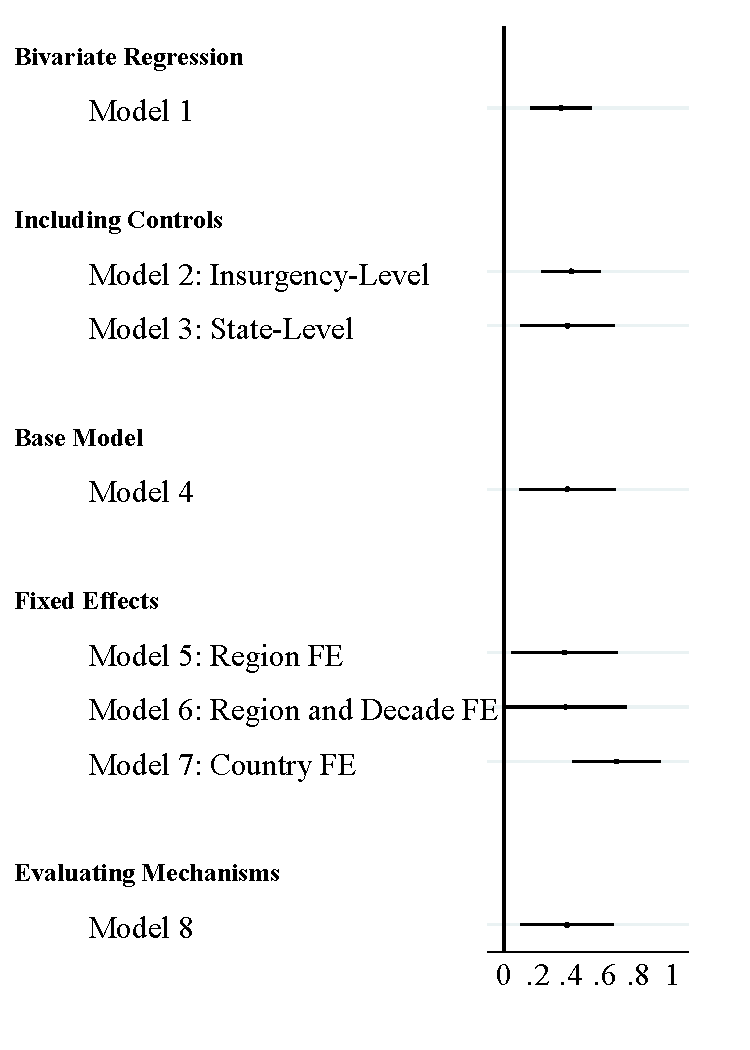
\includegraphics[width=\textwidth]{coefmainpred.pdf}
    \end{subfigure}
% 
	\begin{subfigure}{0.45\textwidth}
    \centering
    \caption{Model 4, \autoref{table:conditional}} \label{figure:mainwithcoef}
    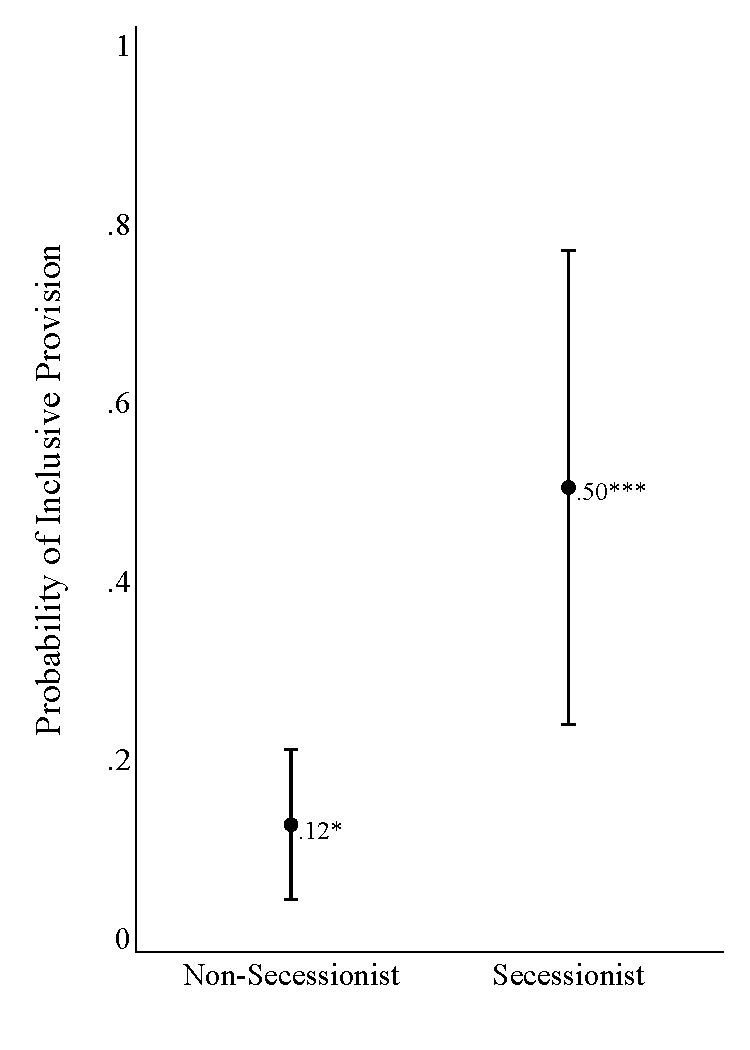
\includegraphics[width=\textwidth]{mainwithcoef.pdf}
    \end{subfigure}
  \begin{tablenotes}[para, flushleft]
\raggedright \footnotesize{\textit{Note:} \autoref{figure:coefmainpred} presents the coefficient estimates for the variable \textit{Secessionist} in \autoref{table:conditional}. Black horizontal lines represent 90\% confidence intervals. If the confidence intervals fail to overlap with the vertical black line, then the effect of \textit{Secessionist} is statistically significant. As can be seen, the results are highly similar, positive and robust across all specifications. \autoref{figure:mainwithcoef} presents the predicted probability of \textit{Secessionist} rebel groups providing inclusive services with all other variables set to their means (Model 4, \autoref{table:conditional}). As is clear, secessionist rebel groups are three times more likely to provide inclusive services than non-secessionist rebel groups. Moreover, the predicted effects of secessionist and non-secessionist goals on the probability of inclusive service provision is statistically significantly different. Vertical lines represent 90\% confidence intervals.}
\end{tablenotes}
\end{figure}



%The results support my hypothesis if the variable \textit{Secessionist} has a positive and statistically significant coefficient. Indeed, the \textit{Secessionist} coefficient is positive with a large substantive effect in all models.  Again, the coefficient for \textit{Secessionist} is positive and statistically significant to the inclusion of these sets of variables. 


%Finally, Table \ref{table:main} reports the results for each of the same model specifications above using the full sample of insurgencies and the interaction of \textit{Secessionist $\times$ Territorial Control} to predict rebel public goods provision. 
%This model demonstrates that the relationship between secessionist rebel groups that control territory and public goods provision is statistically significant and positive without the inclusion of any controls, and remains robust with the incremental inclusion of additional key covariates. I include both insurgency- and state-level controls with region clustered standard errors. Again, the interaction term of \textit{Secessionist $\times$ Territorial Control} is positive and statistically significant at the 99\% level. The direction and significance of the relationship supports the hypothesis that secessionist insurgencies that control territory are more likely to provide public goods. 

%Likewise, \autoref{figure:mainint} presents the predicted probabilities of Model 4, \autoref{table:mainint}. Here, secessionist rebels with territorial control are more than six times more likely to provide inclusive services than non-secessionist rebels, and this difference is statistically significant. Together, this suggests that the results are both statistically significant and substantively meaningful.

%Although non-secessionist insurgencies that control territory are about 7\% likely to provide public goods (45\% less likely to provide public goods than secessionist groups that control territory), this value is not statistically significant, meaning that the value is not statistically distinguishable from a 0\% probability. These results are consistent with the results above, and strongly support the hypothesis. 

%Similarly, Figure 2 presents the results of Model 1, Table \ref{table:conditional}, graphically. When all variables are set to their medians, conditional on controlling territory, secessionist groups are 53\% likely to provide public goods, while non-secessionist groups are neither more nor less likely to provide public goods.\footnote{I set all variables to their medians so that ordinal variables are set to theoretically meaningful levels.} Although non-secessionist insurgencies that control territory are about 7\% likely to provide public goods (45\% less likely to provide public goods than secessionist groups that control territory), this value is not statistically significant, meaning that the value is not statistically distinguishable from a 0\% probability. These results are consistent with the results above, and strongly support the hypothesis. 



\subsection*{Robustness Checks and Predictive Accuracy}

To ensure results are robust to alternative model specifications and to evaluate the predictive accuracy of the model, I include additional diagnostics in Appendices 3-5. Results are robust to using the full sample of insurgencies without conditioning on territorial control; including additional controls; excluding influential observations (outliers, jackknifing); using the unaltered, original NSA Dataset; accounting for information bias in coding; using alternative specifications of the independent variable; using alternative specifications of the dependent variable; using both ordered logit and logistic regression estimators; imputing missing data; replicating the entire analysis (both main tables and appendix tables) using the full NSA panel dataset (Appendix 5). Each of these tests are described in great detail in Appendices 3-5. I evaluate model accuracy using a Receiver Operator Characteristic (ROC)\footnote{\citealt{ward2010perils,young2012repression}} and the bootstrapping technique.\footnote{\citealt{efron1983leisurely, efron1997improvements}} The combined results indicate that the predictive accuracy of both the model and the \textit{Secessionist} variable is very high. 

%To evaluate model fit, I use a Receiver Operator Characteristic (ROC) plot to ascertain the model's ability to correctly predict outcomes and to compare the predictive strength of the key independent variables with other controls. I also estimate the model's ability to predict future out-of-sample observations relying on 

%I conduct a joint significance test to determine whether the \textit{Secessionist} coefficient is statistically different from \textit{Secessionist $\times$ Territorial Control} coefficient and its lower-order terms for the results of Table \ref{table:main}; IThe results of the joint significance test indicate that the coefficients are statistically significantly different.\footnote{${\chi}$-Square=18.52} 

\section*{Conclusion}

In this paper, I argued that inclusive goods provision is a technology of rebellion\footnote{\citealt{kalyvas2010international}} employed by secessionist insurgencies to achieve their long-term goal of independence. When secessionist rebels engage in inclusive service provision, they perform the role of the state and legitimate their sovereign authority domestically and internationally. The results above offer considerable support for this hypothesis.

While much civil war research has focused on territorial control, financial resources, ideology or the path dependent processes that encourage insurgents to develop governing institutions, this work demonstrates how the long-terms goals of insurgencies can shape rebels' strategic calculus and incentivize them to rely on certain technologies as opposed to others. For example, this research echoes recent scholarship that finds that because of secessionist insurgents' long-term goals, they eschew certain types of violence\footnote{\citealt{fazal2013secessionism}} and may be more likely to abide by international norms.\footnote{\citealt{lasley2014secession}} Taken together, this suggests that secessionist insurgencies may operate differently from non-secessionist rebels. Disaggregating between these two categories of civil war may be an important next step in furthering our understanding of intrastate conflict.\footnote{\citealt{lacina2015periphery}} These results also speak to the importance of understanding how and why secessionist insurgencies might eventually be recognized by members of the international community. When secessionist insurgencies provide inclusive goods and control territory, they exercise sovereignty. If other states recognize this sovereignty, then providing inclusive goods could potentially explain why some secessionist groups are more likely receive international recognition of sovereignty, while others do not. In addition, these findings imply that insurgents deploy both nonviolent and violent strategies in tandem, both aimed at achieving their long-term goals. Future research on this topic might turn to explaining sub-national variation in rebel governance, or importantly, why secessionist movements might eschew legitimacy-generating behaviors in favor of violence or ethnic cleansing. 

%This research makes several important contributions to our understanding of civil war and insurgencies. Although previous research has made several important contributions to the study of insurgent strategies of social service provision, these results underscore the importance of disaggregating between populations of beneficiaries. Because different logics undergird insurgents' choice to provide either club or public goods, distinguishing between the two in any analysis is a critical component of ascertaining the determinants of their provision. 

In terms of U.S. foreign policy implications, this work offers insights as to which insurgencies will provide services, and to whom, something that may be critical when addressing the humanitarian consequences of civil war. Additionally, this paper also contributes to peace-building policy as it offers new insights into how existing insurgent institutions may be co-opted in the post-civil war context so that governance vacuums do not arise and critical services continue to be provided to a needy population.

Ultimately, although civil war is frequently understood as anarchical periods of state breakdown, in certain cases, civil wars are actually a conduit for state making. The research presented here offers one potential pathway through which states are born in the post-1945 era. %Relatedly, these results address the importance of the international community, particularly for secessionist civil wars. 

%Second, the results presented here have important implications for the understanding of civil war dynamics, especially rebel strategies. Social service provision is an important sub-set of rebel behaviors, and like insurgents' violent campaigns, their service provision is also strategic. Therefore, integrating research on non-violent behaviors with existing scholarship on rebel violence will paint a more complete picture of civil war dynamics such as civil war termination, insurgent success or failure, civil war duration, civilian targeting and conflict intensity.

%Additionally, these findings provide evidence for a potential need to disaggregate analyses of secessionist insurgencies from revolutions or traditional civil wars. These results, as well as others,\footnote{\citealt{fazal2013secessionism, lacina2013periphery}} suggest that secessionist insurgencies may operate differently from non-secessionist rebels. Disaggregating between these two categories of civil war may be an important next step in furthering our understanding of intrastate conflict. 

%Relatedly, these results also speak to the importance of understanding how and why secessionist insurgencies might eventually be recognized by members of the international community, or said otherwise, how states are born, particularly in the post-1945 era. When secessionist insurgencies provide public goods and control territory, they provide governance and exercise sovereignty. If other states recognize this sovereignty, then public goods provision could potentially explain why some secessionist groups are more likely receive international recognition of sovereignty, while others do not. %Relatedly, these results address the importance of the international community, particularly for secessionist civil wars. 


\newpage
\clearpage
\thispagestyle{plain}
\singlespace
\bibliographystyle{IO_bibstyle}
\bibliography{paperbib}


\newpage
\clearpage
\thispagestyle{plain}
\setcounter{page}{1}
\setcounter{footnote}{0}
\doublespace

\begin{center}
\Large{\textbf{Appendix 1: Descriptive Tables and Figures}}

\let\cleardoublepage\clearpage
\begin{table}[htbp]
\def\sym#1{\ifmmode^{#1}\else\(^{#1}\)\fi}
\setcounter{table}{0}
\renewcommand\thetable{A.\Roman{table}}
\caption{Summary Statistics, Cross-Sectional Data}
\begin{tabular}{l*{1}{cccccc}}
\hline\hline
                    &\multicolumn{6}{c}{}                                                         \\
                    &        Mean&         Median&         Min&         Max&          SD&       Obs.\\
\hline
\textbf{All Insurgencies with Territory} \\
Secessionist        &        0.34&        0.00&        0.00&        1.00&        0.48&         106\\
Communist           &        0.26&        0.00&        0.00&        1.00&        0.44&         106\\
Ethnic War          &        0.06&        0.00&        0.00&        1.00&        0.23&         106\\
Rebel Strength      &        1.15&        1.00&        0.00&        4.00&        0.81&         106\\
Duration            &        9.57&        6.00&        0.00&       54.00&       11.26&         106\\
Infant Mortality    &       88.96&       90.95&        8.20&      254.30&       50.41&          72\\
GDPpc               &        7.21&        6.98&        5.33&        9.88&        1.06&          71\\
Democracy           &        0.22&        0.00&        0.00&        1.00&        0.41&          97\\
Population (logged) &       16.37&       16.26&       13.18&       20.60&        1.51&          85\\
Rugged Terrain      &        2.57&        2.63&        0.00&        4.31&        1.24&         105\\
Competition         &        2.99&        2.00&        1.00&       12.00&        2.29&         106\\
Population (change) &       12.51&       12.69&        8.65&       16.63&        1.54&          72\\\hline
\textbf{Secessionists (Territorial Control)} \\
Communist           &        0.14&        0.00&        0.00&        1.00&        0.35&          36\\
Ethnic War          &        0.00&        0.00&        0.00&        0.00&        0.00&          36\\
Rebel Strength      &        1.03&        1.00&        0.00&        3.00&        0.70&          36\\
Duration            &        9.56&        5.00&        0.00&       54.00&       12.06&          36\\
Infant Mortality    &       73.73&       73.60&        9.90&      176.30&       47.42&          25\\
GDPpc               &        7.30&        7.12&        6.00&        9.08&        0.90&          23\\
Democracy           &        0.20&        0.00&        0.00&        1.00&        0.41&          35\\
Population (logged) &       16.92&       16.66&       13.18&       20.60&        1.88&          30\\
Rugged Terrain      &        2.80&        2.72&        0.00&        4.27&        1.20&          35\\
Competition         &        3.33&        2.00&        1.00&       12.00&        2.92&          36\\
Population (change) &       12.86&       12.79&        9.41&       16.63&        1.98&          22\\
\hline
\textbf{Non-Secessionists (Territorial Control)} \\
Communist           &        0.33&        0.00&        0.00&        1.00&        0.47&          70\\
Ethnic War          &        0.09&        0.00&        0.00&        1.00&        0.28&          70\\
Rebel Strength      &        1.21&        1.00&        0.00&        4.00&        0.87&          70\\
Duration            &        9.57&        6.50&        0.00&       40.00&       10.92&          70\\
Infant Mortality    &       97.06&      100.20&        8.20&      254.30&       50.55&          47\\
GDPpc               &        7.17&        6.89&        5.33&        9.88&        1.14&          48\\
Democracy           &        0.23&        0.00&        0.00&        1.00&        0.42&          62\\
Population (logged) &       16.06&       15.95&       13.22&       18.33&        1.18&          55\\
Rugged Terrain      &        2.46&        2.44&        0.34&        4.31&        1.24&          70\\
Competition         &        2.81&        2.50&        1.00&        7.00&        1.88&          70\\
Population (change) &       12.36&       12.59&        8.65&       14.28&        1.28&          50\\
\hline\hline
\end{tabular}
\end{table}

\newpage
\clearpage

\begin{table}[htbp]
\centering
\small
\setcounter{table}{1}
\renewcommand\thetable{A.\Roman{table}}
\caption{Groups Controlling Territory, Inclusive Services}
 \begin{tabular}{l} 
 \hline
 \hline
Croatian Republic of Bosnia and Herzegovina \\
Dniestr Republic \\
Eritrean People's Liberation Front \\
Sudanese People's Liberation Movement-Nasir Faction \\
Karen National Union \\
Katanga \\
Oromo Liberation Front \\
POLISARIO \\
Republic of Abkhazia \\
Republic of Biafra \\
Republic of Chechnya \\
Republic of Nagorno-Karabakh \\
Republic of South Moluccas \\
Republic of South Ossetia \\
Shan State Army \\
United Front for the Liberation of Assam \\
United Front for the Liberation of Assam Faction \\
Burmese Communist Party \\
FRELIMO \\
Hamas \\
Hezbollah \\
Kurdistan Democratic Party \\
Kachin Independence Army \\
Patriotic Union of Kurdistan \\
Pathet Lao \\
People's Liberation Army \\
Sudanese People's Liberation Movement \\
United Islamic Front for the Salvation of Afghanistan \\
United Wa State Army \\
\hline \hline
\end{tabular}
\begin{tablenotes}[para, flushleft]
\raggedright \footnotesize{\textit{Note:} Coding for whether the group controlled territory from \citep{cunningham2009takes}.} 
\end{tablenotes}
\end{table}

\newpage
\begin{table}[htbp]
\centering
\small
\setcounter{table}{2}
\renewcommand\thetable{A.\Roman{table}}
\caption{Groups Controlling Territory, No Inclusive Service Provision}
 \begin{tabular}{l} 
\hline \hline
Anya Nya \\
Bougainville Revolutionary Army \\
Alliance of Democratic Forces for the Liberation of Congo \\
Conseil National de Liberation \\
Communist Party of India (Maoist) \\
Communist Party of Nepal-Maoist/United People's Front \\
Communist Party of Malaya \\
Democratic Army of Greece \\
Eritrean Liberation Front \\
Ethiopian People's Revolutionary Party \\
Eritrean Liberation Front \\
Free Aceh Movement \\
Zapatista Army of National Liberation \\
Armed Forces of the North \\
Fuerzas Armadas Revolucionarias de Colombia \\
Congolese National Liberation Front \\
Farabundo Marti National Liberation Front \\
Front for the Restoration of Unity and Democracy \\
Sandinistas \\
National United Front of Kampuchea \\
Hukbalahap Rebellion \\
Independent National Patriotic Front of Liberia \\
Nasserite Movement \\
Indonesian Peoples Army \\
Khmer Issarak \\
Kurdistan/KDPI (1946) \\
Lebanese Front \\
Lebanese National Movement \\
Liberation Tamil Tigers of Eelam \\
Movement of Democratic Forces of Casamance \\
Mouvement Populaire de l'Azaouad \\
Mong Tai Army \\
Mukti Bahini: Liberation Force \\
Democratic Movement for Malagasy Restoration \\
Mouvement Pour la Justice et la Paix \\
Mouvement pour la Liberation du Congo \\
Mouvement Patriotique de Cote d'Ivoire \\
Mon People's Front \\
Mouvement Populaire des Ivoiriens du Grand Ouest \\
Free Papua Movement \\
Muslim Brotherhood \\
\hline
\hline
\end{tabular}
\begin{tablenotes}[para, flushleft]
\raggedright \footnotesize{\textit{Note:} Coding for whether the group was secessionist and whether the group controlled territory from \citep{cunningham2009takes}.} 
\end{tablenotes}
\end{table}

\newpage
\begin{table}[htbp]
\begin{center}
\small
\setcounter{table}{2}
\renewcommand\thetable{A.\Roman{table}}
\caption{Groups Controlling Territory, No Inclusive Service Provision (Cont.)}
 \begin{tabular}{l} 
National Liberation Front \\
New People's Army \\
National Patriotic Front of Liberia \\
National Liberation Army \\
Free Oman Movement \\
People's Front for the Liberation of Oman and the Arab Gulf\\
Rally for Congolese Democracy \\
Rally for Congolese Democracy (Faction) \\
Revolutionary United Front \\
Renamo \\
Somali National Movement \\
Shan State Independence Army \\
Tigrayan People's Liberation Front \\
Taliban \\
Tibet \\
United Lao National Liberation Front \\
National Union for the Total Independence of Angola \\
Ushtria Clirimtare e Kosoves \\
Ukrainian Insurgent Army \\
National Revolutionary Movement \\
United Somali Congress (Faction) \\
Ushtria Clirimtare e Kosoves \\
Viet Nam Doc Dong Min Hoi \\
Zviadists \\
\hline \hline
\end{tabular}
\begin{tablenotes}[para, flushleft]
\raggedright \footnotesize{\textit{Note:} Coding for whether the group controlled territory from \citep{cunningham2009takes}.} 
\end{tablenotes}
\end{center}
\end{table}

\newpage
\clearpage

\Large{\textbf{Appendix 2: Controls}}
\end{center}

\normalsize 

In most models, I add insurgency-level control variables that may impact whether a rebel group provides inclusive services. In his text \textit{On Guerrilla War}, Mao Tse-Tung writes that insurgencies need a popular base of support in order to survive, and it is from this base that they derive their strength.\footnote{\citealt[43-4]{tse2000guerrilla}} As a result, Mampilly (2011) has hypothesized that Maoist groups are more likely to provide social services.\footnote{\citealt[78-9]{mampilly2011rebel}} Moreover, these groups may be more inclined to rely on guerrilla strategies and seek out certain types of territory that convey a tactical advantage (mountains, swamps, jungles, etc.). To account for the ideological influence of Mao on other insurgent groups, I created a variable called \textit{Communist} if a group had a socialist or communist ideology. Data from this variable originate from the NSA Dataset casebook. If the NSA Dataset casebook refers to a group as ``Marxist,'' ``Maoist,'' ``communist'' or ``socialist,'' the observation receives a ``1'' meaning communist, and a ``0'' if otherwise.  I also triangulate this coding with the \textit{Communist} variable from the ``Technologies of Rebellion''  dataset,\footnote{\citealt{kalyvas2010international}} which codes all civil wars that had at least one communist insurgency.  

Additionally, some ethnic wars are secessionist wars, while almost all secessionist wars have an ethnic component. To ensure that secessionism drives the results, and not ethnicity, I include the variable \textit{Ethnic War}. This variable comes from the NSA Dataset's variable \textit{ethnic}. It is coded as a ``1''  if a civil war is an ethnic war, but not a secessionist war. If ethnicity truly drove the results, then non-secessionist, ethnic wars should be associated with a greater likelihood of providing more inclusive governance. Otherwise, coding both secessionist and non-secessionist ethnic wars introduces collinearity. 

Another key factor that may incline rebel groups to provide inclusive services is military strength. The strength of a rebel group might positively or negatively impact its propensity to provide inclusive goods. Weinstein\footnote{\citealt{weinstein2006inside}} argues that groups lacking economic endowments are more likely to provide social services. Similarly, groups lacking military strength may heavily rely on the civilian population for support. As a result, inclusive goods provision could be a weapon of the weak, employed to generate support amongst, and harvest supplies from, the population in which an insurgency is embedded. The National Revolutionary Movement (NRM) in Uganda, for example, began with few military resources and just 27 men, but soon provided social services within the territory it controlled.\footnote{\citealt[68]{weinstein2006inside}} This suggests that lower levels of rebel group strength will correspond to an increased likelihood of providing inclusive goods. Alternatively, social service provision could be seen as a corollary of strength: only strong groups have the necessary resources, training and capacity to provide inclusive services. In this case, one would expect rebel group strength and inclusive goods to have a positive relationship with inclusive service provision, indicating that stronger insurgencies are more likely to provide services inclusively. I include a measure of rebel strength from the NSA Dataset, with each insurgent group coded as ``much weaker,'' ``weaker,'' ``parity,'' ``stronger,'' or ``much stronger,'' in comparison to the incumbent government they are fighting (operationalized as an ordinal variable ranging from ``0'' to ``4,'' respectively). 

%I include a measure of \textit{Central Command Strength} from the variable ``Strength of Central Command''  in the NSA Dataset. The NSA Dataset lists the values of this variable as ``high,'' ``moderate,'' ``low,'' or ``unclear.'' To operationalize this variable for statistical analysis, I code the \textit{Central Command Strength} variable as ``0'' if the rebel group had ``low'' central command strength, ``1'' if the rebel group had ``moderate'' central command strength and ``2'' if the rebel group had high central command strength. I code as missing any variables that are listed as ``unclear'' in the NSA Dataset. 

%I include the \textit{Central Command Strength} variable for two reasons: first Weinstein\footnote{\citealt{weinstein2006inside}} argues that groups lacking economic resources must be highly disciplined and ideologically driven to attract new members. These highly disciplined organizations use social services to attract recruits. Thus, insurgencies with high levels of central command strength may reflect groups lacking economic resources. These groups are in turn more likely to provide public goods. 

%Second, Staniland\footnote{\citealt{staniland2014networks}} argues that ``integrated'' and ``vanguard'' insurgent organizations are more likely to have strong central command structures, compared to ``parochial'' and ``factional'' groups. ``Integrated'' rebel groups are likely to have close ties across leaders within the rebel organization, but also to local populations outside the organization. These strong horizontal and vertical ties might make groups more inclined to strategize about social service provision, then implement them locally. Meanwhile, ``vanguard'' organizations may be less likely to provide social services unless the state is absent.\footnote{\citealt[46]{staniland2014networks}} Parochial and fragmented groups with low central command strength may be less likely to provide social services because parochial groups already have strong ties to the local population and so do not need to provide social services, while fragmented groups are unlikely to build strong ties with leaders within the organization or locally due to organizational dysfunction.\footnote{Ibid, 53} Thus one would predict that groups with a weaker central command, such as parochial or fragmented groups, are less likely to provide social services while integrated and vanguard organizations with a strong central command may be more likely to provide social services. 

%I code the ordinal variable \textit{Rebel Strength}  as ``0'' if rebel strength is listed as ``much weaker,''  a ``1'' if the group's strength is listed as ``weaker,'' a ``2'' if the organizational strength is at ``parity'' with the state, a ``3'' if the rebel group is ``stronger'' than the incumbent government and a ``4'' if the rebel group is coded as ``much stronger'' than the state it is fighting. 




Finally, I include the variable \textit{Duration} which measures the number of years a rebel group operated. Some insurgencies may not provide inclusive services, let alone any services, simply because they achieve victory too quickly and do not have time to establish these institutions. To account for the  time rebels needed to establish their governance, I include this measure. 

Insurgencies do not operate within a vacuum, and state-level attributes could be critical determinants of inclusive goods provision. The regime type of the incumbent regime could also influence rebels' propensity to provide inclusive services. Because democracies foster electoral participation and competition,\footnote{\citealt{mulligan2004democracies}} insurgencies may need to develop a broader base of support. To create this broad coalition, insurgencies may provide services inclusively. To account for this, I include a binary indicator variable for whether a country is a \textit{Democracy} (coded as ``1''  if the country is a democracy and a ``0'' otherwise) from Cheibub, Gandhi and Vreeland.\footnote{\citealt{cheibub2010democracy}}

The level of social development may also impact inclusive goods provision because lower levels of social development means populations have a greater need for services. Insurgencies may be incentivized to provide more inclusive goods when the population has a greater need for these services. Consistent with previous research,\footnote{\citealt{girod2012effective}} I measure social development with the \textit{Infant Mortality Rate} variable from the \citet{world2012}. Additionally, high levels of state capacity and economic strength may make it more difficult for an insurgency to begin a civil conflict or control territory. However, a stronger state may produce the personnel resources (educated teachers and doctors) to staff an insurgency's social service apparatus. To account for this, I include the variable \textit{GDPpc}, a logged measure of GDP per capita\footnote{\citealt{fearon2003ethnicity}} from Penn World Tables.\footnote{\citealt{heston2002penn}} Measures of extractive capacity or political capacity would better approximate state strength,\footnote{\citealt{hendrix2010measuring}} however, these data are geographically and temporally limited, so I use GDP per capita which has greater coverage and does not reduce the sample size drastically. 

%Additionally, states facing worsening economic conditions may close schools or hospitals, in turn opening up a space for insurgents to provide services. Insurgencies operating in states with a decline in GDP per capita may be more likely to provide public goods to fill this governance gap. As such, I include a measure of \textit{Income Growth} operationalized as the rate of change in GDP per capita from one year to the next, calculated from Penn World Tables.\footnote{\citealt{heston2002penn}} 

If insurgents operate in a highly populated area, it may limit their ability to provide inclusive services as the insurgency might require a greater capacity and more resources to meet the demands of that population. Therefore, I include the variable \textit{Total Population (Logged)} from Penn World Tables.\footnote{\citealt{heston2002penn}} I also include measures of \textit{Rugged Terrain}\footnote{\citealt{fearon2003ethnicity}} as a mountainous landscape might make it more difficult for states and insurgencies to control territory, and thus it may also complicate both a state's and an insurgency's ability to provide inclusive goods. Additionally, if insurgents, especially non-secessionist rebels, choose territorial spaces that confer tactical advantage (like mountains or jungles) but are depopulated, this would suppress the ability of insurgents operating in these areas to provide services inclusively. 

Finally, in some models, I include two variables to address rival mechanisms. The first variable is \textit{Competition}, a count of the maximum number of rebel groups simultaneously operating in the same country. If inclusive goods provision is a response to intensifying rivalries, an increase in the number of rebel groups should correspond to an increase in the likelihood of inclusive service provision. This count measure was created from the NSA Dataset (2009). Second, I include the variable \textit{Population (Change)} to account for insurgencies' desire to prevent out-migration. Created using data from Penn World Tables, \textit{Population (Change)} measures fluctuations in a country's population from one year to the next. Decreases in the population should correspond to an increased likelihood of insurgencies providing services inclusively.

%Because I hypothesize that secessionist insurgencies are more likely to provide public goods, states that have high levels of ethnic fractionalization may be more likely to experience secessionist wars in the first place. If the results support the hypothesis that territory-controlling secessionist insurgencies are more likely to provide public goods, \textit{Ethnic Fractionalization} may be a confounding factor. Second, \textit{Rugged Terrain} 
%Finally, the Cold War has been shown to be associated with different modes of civil conflict.\footnote{\citealt{kalyvas2010international}} To account for the effects the Cold War may have on public goods provision, I include the variable \textit{Cold War}, coded as ``1'' if the year is between 1945 and 1991 and a ``0'' if the year is 1992 or later. Additionally, because Weinstein\footnote{\citealt{weinstein2006inside}} has hypothesized that high levels of economic endowments make insurgencies less likely to provide social services, state sponsorship of various insurgencies during the Cold War may make insurgencies during this time period less likely to provide public goods.\footnote{\citealt{salehyan2014external}}

\begin{table}[h]
\def\sym#1{\ifmmode^{#1}\else\(^{#1}\)\fi}
\renewcommand\thetable{A.\Roman{table}}
\caption{\textbf{Summary of Controls and Coding}}
    \begin{tabular}{| c | c | c |}
    \hline
    \textbf{Variables} & \textbf{Original Variable} & \textbf{Operationalization} \\ \hline \hline
    Inclusive Services &                NA                  & 1=Inclusive education, health \\
    &  &  0=No Inclusive Services  \\ \hline
 Secessionist &  21 unique conflict types  & 1=``Secessionist,'' \\
  &   (NSA Dataset, 2009) & ``Ethnic Conflict/Secessionist,'' \\
   &   & ``Civil War/Secessionist,''   \\
    &      & and ``Secessionist/Terrorist'' \\ 
     &    & 0=All other conflict types  \\  \hline
Territorial Control &   ``Yes''   or  ``No''                & 1=Territorial control\\
      &   (NSA Dataset, 2009) &  0=No territorial control     \\
          \hline
Communist &                NSA Case notes/               & 1=Communist\\
      & \citep{kalyvas2010international} &  0=Not communist  \\ \hline
Ethnic War &       ``ethnic'' variable & 1=Ethnic, non-secessionist war \\   
 &       (NSA Dataset, 2009)          &  0=Not ethnic or secessionist war  \\       \hline     
Duration &         Year  (NSA Dataset 2009)             & Number of years an   \\  
&                    &   insurgency existed  (count)\\        \hline
Rebel Strength & ``rebstrength'' variable & 0-4 range: \\
 &  ``Much Stronger'' & 0=Much Weaker, \\
  &  ``Weaker'' & 1=Weaker, \\
   &   ``Parity'' &  2=Parity, \\
    &   ``Stronger''  & 3=Stronger, \\ 
     &  ``Much Stronger''  & 4=Much Stronger \\  
       &  (NSA Dataset, 2009) &  \\    \hline
 Infant Mortality &       Infant Mortality Rate               & Infant Mortality Rate\\      
  &        \citep{world2012}         &  \\   \hline

GDPpc&       GDP per capita              & Log of GDP per capita\\       
 &        (Penn World Tables 2012)          &  \\   \hline
 Democracy &           Democracy Variable         & 1=Democracy\\   
 &         \citep{cheibub2010democracy}           & 0=Non-Democracy   \\   
 &                  & \\          \hline     
Population (Logged) &       Total Population                & Total Population (Logged) \\  
&      \citep{heston2002penn}              & \\        \hline
Rugged Terrain &      Log of Mountainous Terrain             & Log of  \\   
 &       \citep{fearon2003ethnicity}          & Mountainous Terrain \\         \hline  
 Competition &       Number of insurgencies operating        & Rebel groups (count) \\  
&       simultaneously in a country            & \\        
&       (NSA Dataset, 2009)            & \\        \hline
 Population (Change) &         Total population              & Change in population (logged) \\  
&       \citep{heston2002penn}                 & from one year to the next \\        \hline

 \hline
    \hline
    \end{tabular}
\end{table}



\newpage
\clearpage
\begin{center}
\Large{\textbf{Appendix 3: Robustness Checks}}
\end{center}

In this section, I describe the results of several robustness checks in greater detail. Across all models, the \textit{Secessionist} coefficient remains positive and statistically significant, indicating that the relationship between secessionist long-term goals and inclusive service provision is strong. I describe each robustness check more fully below. 

%\begin{figure}[h!]
%\centering
%\begin{center}
%\renewcommand\thefigure{A.\arabic{figure}}
%\caption{Secessionist Coefficient Estimates Summary, Logit Models}
%\label{figure:coef}
%\scalebox{1}{\includegraphics{coef.pdf}}
%\end{center}
%\begin{tablenotes}[para, flushleft]
%\raggedright \footnotesize{\textit{Note:} The figure presents a summary of the \textit{Secessionist} coefficient estimates for all robustness checks that rely on a logistic estimator. If no black standard error bars or black markers cross the vertical zero line, we can be confident that the variable  \textit{Secessionist} remains positive and statistically significant across all robustness checks. These findings strongly support the hypothesis and increase the confidence in findings .} 
%\end{tablenotes}
%\end{figure}

%\begin{figure}[h!]
%\centering
%\begin{center}
%\renewcommand\thefigure{A.\arabic{figure}}
%\caption{Secessionist Coefficient Estimates Summary, OLS Models}
%\label{figure:coefols}
%\scalebox{1}{\includegraphics{coefols.pdf}}
%\end{center}
%\begin{tablenotes}[para, flushleft]
%\raggedright \footnotesize{\textit{Note:} The figure presents a summary of the \textit{Secessionist} coefficient estimates for all robustness checks that rely on a linear probability model. If no black standard error bars or black markers cross the vertical zero line, we can be confident that the variable  \textit{Secessionist} remains positive and statistically significant across all robustness checks. These findings strongly support the hypothesis and increase the confidence in findings .} 
%\end{tablenotes}
%\end{figure}


%because of the time invariant construction of certain insurgency- and state-level variables, I cannot include insurgency fixed effects and obtain estimates for the \textit{Secessionist} variable, the key independent variable. Moreover, including country-level fixed effects presents a challenge due to the time-invariant nature of the key independent variable. When country fixed effects are included, only countries that simultaneously experience secessionist insurgencies with territorial control  and non-secessionist insurgencies with territorial control appear in the model (six total countries). Theoretically meaningful time-invariant country-level variables must also be excluded from the model, meaning that \textit{Rugged Terrain} and (due to the small sample size) \textit{Democracy} must be excluded from the model. However, the coefficient for \textit{Secessionist} remains positive and robust, further supporting the hypothesis (Model 1, Appendix Table \ref{table:asefe}). In addition, Models 2 and 4 of Appendix Table \ref{table:asefe} present the results using the same specification as Model 7, Table \ref{table:conditional}, but instead uses standard errors clustered by insurgency and region (respectively), as opposed to country while Models 3 and 5 present the results using the same specification as Model 6, Table \ref{table:conditional}, but instead uses decade fixed effects and standard errors clustered by insurgency and region (respectively). Finally, Model 6 includes insurgent-level random effects. Even with these alternative fixed effects and clustered standard errors specifications, \textit{Secessionist} is still large, positive and statistically significant, adding further support for the hypothesis. 

%Including However, to show that the results are robust to the inclusion of fixed effects, in Models 1 and 2 of Appendix Table A.III, I include region fixed effects with standard errors clustered by region (Model 1) and conflict (Model 2). The Model 2 specification accounts for differences across regions and inflates standard errors by conflict to correct for unobserved correlation in the error term within conflicts. Models 3 and 5 of Appendix Table A.V exclude the \textit{Cold War} variable and include year fixed effects and region fixed effects, clustering standard errors on region (Model 3) and conflict (Model 5). Models 4 and 6 include the \textit{Cold War} variable and year fixed effects, and cluster errors on region (Model 4) and conflict (Model 6). 

First, in Appendix Table \ref{table:mainint}, I replicate \autoref{table:conditional} in the main text, but use the full sample of insurgencies. I interact the \textit{Secessionist} variable with the \textit{Territorial Control} variable. The positive and statistically significant coefficient for \textit{Secessionist} $\times$ \textit{Territorial Control} supports the hypothesis that when secessionist rebels control territory, they are more likely to provide inclusive services. \autoref{figure:coef} and \autoref{figure:main} present a side-by-side comparison of the predicted effect of secessionism on inclusive governance using both the stratified sample (\autoref{figure:coefmain} and \autoref{figure:mainc}) and the full sample of insurgencies (\autoref{figure:coefmainint} and \autoref{figure:mainint}). Because there are so few observations in \autoref{table:conditional}, this robustness check is particularly valuable.




Next, in Appendix Table \ref{table:addcontrols1}, I include additional controls that might impact the likelihood that secessionist insurgencies with territorial control provide inclusive goods. In each model of Appendix \autoref{table:addcontrols1}, I include an additional control variable, before including all additional control variables in Models 9-12 of Appendix \autoref{table:addcontrols2}. In Model 1, I replace the \textit{Population (Logged)} variable with \textit{Population Change (Logged)}. The results do not support the out-migration hypothesis, while the \textit{Secessionist} variable remains positive and statistically significant. 

Because Weinstein\footnote{\citealt{weinstein2006inside}} predicts that groups with high levels of economic endowments are less likely to provide social services, insurgencies receiving external monetary support may also be less likely to provide social services.\footnote{\citealt{salehyan2014external}} Therefore I include a measure for whether a group received non-military aid in Model 2, Appendix \autoref{table:addcontrols1}. To code this \textit{Non-Military Aid} variable, I used the NSA Dataset in conjunction with UCDP's External Support Dataset.\footnote{\citealt{hogbladh2011external}} I code \textit{Non-Military Aid} as ``1'' if the NSA Dataset  lists the observation as receiving ``non-military aid,'' as opposed to an ``endorsement,'' ``troops'' or ``military aid.'' As some observations might receive two types of aid, I also code the \textit{Non-Military Aid} variable as  ``1'' if the UCDP External Support Dataset codes the observation as receiving economic aid in that year.\footnote{While an important theoretical variable, because many observations are missing, it reduces the sample size significantly, and so I do not include it in the base models (Models 4-7, Table 1).} The results are robust to the inclusion of the \textit{Non-Military Aid} variable. 

Model 3 of Appendix Table \ref{table:addcontrols1} includes the variable measure \textit{Rebel Size}, operationalized as the log of the best estimate of rebel size from the NSA Dataset. A larger rebel group may be more likely to provide services inclusively because the rebel group has enough people to fill both combat and non-combat positions. Even with the inclusion of the variable \textit{Rebel Size}, \textit{Secessionist} is still positive, large and statistically significant. 

In Model 4 of Appendix Table \ref{table:addcontrols1}, I control for the logged number of \textit{Battle Deaths}, as groups that commit more violence may use inclusive services to attract recruits more willing to commit greater violence.\footnote{\citealt{berman2008religion}} Using data from \citet{lacina2005monitoring}, this variable is operationalized as the log of the maximum best estimate of the number of battle deaths that occurred in any year of a rebel group's existence. When the best estimates were not available, I used the maximum low estimate. Even with the inclusion of this variable, the \textit{Secessionist} coefficient is still robust and positive, further supporting my argument. 

Model 5 includes the measure \textit{Competition} for the maximum number of other insurgencies operating within the same country at the same time. Again, however, the \textit{Secessionist} coefficient retains its strong positive result. 

Models 6 and 7 of Appendix Table \ref{table:addcontrols1} presents the results of the inclusion of the control variables \textit{Pre-Conflict Education} and \textit{Pre-Conflict Health}. The \textit{Pre-Conflict Education} and \textit{Pre-Conflict Health} variables measure whether the group provided \textit{any} education or any healthcare prior to the onset of civil war. This does not mean a rebel group provided inclusive education or healthcare, but it could mean they provided healthcare for combatants or core members. For example, rebels may be hidden away in the hinterlands training and participating in literacy or mathematics courses, prior to launching any violent campaign. On the other hand, it could suggest that some rebel groups provided services but had not committed enough violence to be considered an active insurgency. These variables are coded as a ``1'' if the rebel group provided any education or healthcare prior to conflict onset, and a ``0'' if they did not. The \textit{Secessionist} coefficient is still positive and robust. 

In Model 8 of Appendix Table \ref{table:addcontrols1}, I create binary indicator variables for each category of rebel group strength (five total categories ranging from ``Much Weaker'' to ``Much Stronger''). I include each of these categorical indicators (except one, ``Much Stronger,'' which is used as a reference category). The \textit{Secessionist} variable remains positive and statistically significant.

Finally, I include all additional control variables in Models 9-12 of Appendix Table \ref{table:addcontrols2} as a difficult test for the hypothesis, and I include region, and region and decade fixed effects (Models 11 and 12, respectively). Across all specifications, \textit{Secessionist} is positive and statistically significant despite the inclusion of seven additional control variables and the related decrease in observations due to the missingness of these data in an already small dataset. The results strongly support the hypothesis that territory-controlling secessionist insurgencies are more likely to provide inclusive goods. 

%Although it is unlikely that the results are a product of endogenous processes, it is not impossible that endogeneity may be effecting the results. Endogeneity may occur if an organization provides inclusive services, then becomes a secessionist insurgency that controls territory. Secessionism is more likely to occur under certain conditions where economic, normative and security benefits of secession are high and not because of inclusive service provision,\footnote{\citealt{sambanis2014explaining, fazal2014membership}} but one could argue that cases such as the Republic of Nagorno-Karbagh, South Ossetia or Abkhazia are examples of organizations that provided inclusive goods and controlled territory, then decided to rebel and raise secessionist armies.  Model 1 of Appendix Table \ref{table:exclude} reports the logistic regression model after excluding all cases where rebel groups enjoyed considerable governing autonomy, such as former Soviet \textit{oblasts} or republics, prior to the onset of civil conflict. The coefficient for \textit{Secessionist} is statistically significant and robust, consistent with the hypothesis. 

%For an even tougher test, I re-estimate the logistic regression model excluding all cases that enjoyed considerable governing autonomy prior to conflict onset, as well as all observations that provided public goods prior to the official onset of civil conflict (Appendix Table A.V, Model 2). This test is tougher as some insurgencies are not coded as engaging in civil conflict unless they have caused a certain number of battle deaths. Thus, even if an insurgency exists and has committed violence, if the level of violence is too low, the insurgency may not enter the NSA Dataset \citeyearpar{cunningham2009takes}. For example, Hezbollah has engaged in violence since 1982 and began providing public goods in the mid-to-late 1980s, but does not enter the dataset until 1990. Even with this extremely difficult test, the results are still robust and support the hypothesis.     

Next, to ensure that the results are not the results of outliers or influential observations, I re-estimate the base model excluding all outliers (Model 1, Appendix Table \ref{table:outliers}). To determine the cases that are outliers, I calculate the Cook's D of each observation in the sample. The Cook's D measures the leverage of each observation. Typically, if an observation has a Cook's D higher than 4/\textit{n} where ``\textit{n}'' equals the number of observations, the observation is considered an outlier and excluded. After identifying all outliers, I re-estimate the model excluding these observations. The coefficient of \textit{Secessionist} is statically significant and positive, supporting the hypothesis. 

I also analyze the data using a ``jackknife" estimation technique. Jackknifing entails dropping a single observation from the sample and re-estimating the model, generating predicted coefficients and standard errors. Once the model has been estimated, the observation is replaced, the next observation is excluded, and the model is re-estimated. This process is repeated until all observations have been excluded, at which point the coefficients and standard errors are recalculated. Again, the \textit{Secessionist} coefficient is robust (Model 1, Appendix Table \ref{table:jackknife}). 

The dataset I use reflects updates to the original NSA Dataset in lieu of new information. These updates include changing the coding of territorial control of Hezbollah, Hamas and the Ethiopian People's Revolutionary Party as well as eliminating the conflict type of ``terrorist'' which lacked analytic utility. I use alternative conflict-type categories already existing in the NSA Dataset to re-code this variable. Seven rebel groups including Hamas, Hezbollah, Al-Aqsa Military Brigades, Popular Front for the Liberation of Palestine (PFLP), Popular Front for the Liberation of Palestine-General Command (PFLP-GC), National Organization of Cypriot Fighters (EOKA) and Devrimci Sol were coded as terrorist groups only. All but three of these groups are Palestinian liberation organizations. The Palestinian liberation groups are re-coded as ``independence/anti-occupation'' organizations. Because Hezbollah formed in response to the Israeli occupation and also sought to overthrow the Lebanese government until 1990, Hezbollah is coded as ``anti-occupation/civil war.'' The EOKA operating in Cyprus is coded as an ``anti-colonial'' organization as it sought to overthrow Turkish influence. The Devrimci Sol group sought to implement communism in Turkey, and so it is coded as a ``communist'' conflict. To demonstrate that these updates to the data do not bias the results, I re-estimate the model using the unchanged NSA Dataset. Again, the results are still robust: the \textit{Secessionist} coefficient is positive and statistically significant, supporting the theory (Model 1, Appendix Table \ref{table:original}).

%In the models above, I constructed ordinal variables from the original ordinal text-based codings of the variable \textit{Rebel Strength}. In Appendix Table \ref{table:altcontrol}, I instead use indicator variables for each level of \textit{Rebel Strength} (much weaker, weaker, parity, stronger, much stronger). The positive and statistically significant coefficient for \textit{Secessionist} indicates the results are robust to this alternative control variable specification.  

Because the dependent variable is hand-coded with global coverage of all insurgencies dating back over 70 years, there may be concerns that results are biased as a result of the available information, or a lack thereof. To address these concerns, I conduct three additional tests. First, in Model 1 of Appendix \autoref{table:info}, I limit my sample further to only insurgencies that: 1) controlled territory and 2) had a group size greater than the average (mean) group size of insurgencies that controlled territory. Because there may be limited information available about rebel groups that were smaller, these small insurgencies may be coded as missing or as no service provision, when in fact they did provide services, even inclusive services. By limiting the sample to only large insurgencies, this eliminates the possibility that the results are biased because of a lack of information about small rebel groups. In Model 2 of Appendix \autoref{table:info}, I limit my sample again to only insurgencies that operated after 1970 and controlled territory. Here again, there may be a lack of information about rebel groups that existed at earlier time periods. By stratifying my sample, I account for this potential source of bias. Again, results remain robust. Finally, in Model 3 of Appendix Table \ref{table:info} I present the results when missing values for inclusive service provision are replaced with ``0.'' This serves as a check against missing observations needing to be accurately coded as ``0.'' Across all models in Appendix \autoref{table:info}, results are positive and statistically significant suggesting that information bias was not driving the results of my analysis. %If the precise year of when insurgencies began providing inclusive goods was unclear, preceding values were coded as missing.\footnote{For example, the Karen National Union was providing inclusive education and health in 1976, but how far in advance before that time is unclear. In Model 3, I replace these missing values with ``0'' so that they are included in the analysis} 

To ensure that my operationalization of secessionist groups is not too narrow, I develop three alternative specifications of secessionist rebel organizations. Secessionists as well as anti-occupation and anti-colonial insurgencies may all view their state as being controlled by a ``foreign'' ruler. Each of these types of groups might seek to overthrow the ``foreign'' ruler and govern the occupied or colonized state independently. Using the NSA Dataset, if any group's conflict type includes the term ``Secessionist'' or ``Anti-Colonial,'' it is coded as \textit{Secessionist, Broadly Defined} in Model 1 of Appendix Table \ref{table:altsec}. In Model 2, \textit{Secessionist, Broadly Defined} includes secessionist, anti-occupation, and anti-colonial conflict types.\footnote{From the NSA Dataset ``Conflict Type'' variable.} Finally, because autonomy conflicts seek an increase in regional power while eschewing outright independence, it is similar to, although not precisely the same as, secessionism. Thus, I include autonomy conflicts, secessionist conflicts, anti-colonial conflicts and anti-occupation conflicts\footnote{Also from the NSA Dataset ``Conflict Type'' variable.} in the final measure of \textit{Secessionist, Broadly Defined} (Model 3, Appendix Table \ref{table:altsec}). In all three models, the variable \textit{Secessionist, Broadly Defined} is positive and statistically significant, consistent with the hypothesis. 

While the results of the alternative specification of the independent variable are robust, to ensure that results are not simply an artifact of coding the dependent variable, I analyze the same statistical model using an alternative measure of inclusive service provision (Appendix Table \ref{table:altpg}). In Model 1 of Appendix Table \ref{table:altpg}, I code a group as providing inclusive goods if the organization provided either inclusive education or healthcare. This is a lower threshold of inclusive goods provision because organizations need only provide one service inclusively.\footnote{This coding also increases the number of observations that can be included in the model. This is because in the original measure of inclusive goods provision I use demands that both education and healthcare variables are not missing. For Model 1 of Appendix Table \ref{table:altpg}, if either education or healthcare variables are not missing, this observation is included in the model.} Even with this lower threshold, the results continue to support the hypothesis, due to the positive and statistically significant \textit{Secessionist} coefficient. 

As noted in the sections above, any questionable cases I encountered while coding were first coded as the best estimate and then as an alternative coding. In Model 2 of Appendix Table \ref{table:altpg}, I replace the best estimate with the alternative, secondary measure if a case was questionable or marginal. Despite this alternative specification of the dependent variable, the \textit{Secessionist} coefficient is robust with a statistically significant and positive coefficient, providing further evidence in support of the theory.  

In Model 3 of Appendix Table \ref{table:altpg}, I replace the binary \textit{Inclusive Service Provision} variable with an ordinal measure raining from ``0'' to ``2'' that represents the various categories of beneficiaries included in the Insurgent Social Services Dataset. A ``0'' represents no services; a ``1'' signifies provision to insurgents, supporters and non-affiliated civilians likely to support the insurgency; while a ``2'' signifies that insurgents provided services inclusively. A positive and statistically significant coefficient for the \textit{Secessionist} term supports the hypothesis. Again, the results are robust to this alternative specification. 

Appendix Tables \ref{table:altsec} and \ref{table:altpg} demonstrate that the results are not an artifact of the construction of the independent or dependent variables. To ensure that the results are not driven by my use of a Linear Probability Model (LPM), however appropriate this estimator may be, I re-estimate the analysis employing a logistic regression estimator (Model 1, Appendix Table \ref{table:altest}). Next, in Model 2, I use the ordinal construction of \textit{Inclusive Service Provision} from Model 3 of Appendix Table \ref{table:altpg}, but I use an ordered logistic regression estimator to estimate the effects of \textit{Secessionism} on more inclusive governance.  Again, the results are robust, statistically significant, and positive. 

Finally, the country-level control variables induce considerable missigness. To ensure that results are not an artifact of the missingness generated from the inclusion of these control variables, I use multiple imputation by chained equations in Appendix \autoref{table:micec}. In these models, I create 20 imputations of the variables \textit{GDP per capita, Democracy, Infant Mortality Rate,} and \textit{Total Population.} Results are robust and the predicted effect size of being a secessionist group is approximately the same as the predicted effect presented in \autoref{table:conditional}. 

%but the substantive effect is consistent in both models. The \textit{Secessionist} coefficient of Model 1 of Appendix \ref{table:ols} shows that a secessionist group that controls territory is 31 percentage points more likely to provide inclusive goods than a non-secessionist group that controls territory.  This is not substantially different from the predicted effect in the logistic regression model (Model 4, Table \ref{table:conditional}). 

%Finally, in a separate set of regressions (Appendix Table \ref{table:main}), I re-estimate almost the same models as those presented in Table \ref{table:conditional} but I include all insurgencies in the dataset. Using this full sample, I interact the \textit{Secessionist} variable with the \textit{Territorial Control} variable. The statistically significant positive coefficient of this interaction term across all models in Appendix Table \ref{table:main} indicates that secessionist insurgencies that control territory are more likely to provide inclusive services. 

%Figure \ref{figure:fullprob} presents the predicted probabilities of Model 4 in Appendix Table \ref{table:main}.  With all variables set to their means, the results indicate that secessionist insurgencies that control territory are 51\% likely to provide inclusive services. This means that secessionist rebels with territory are about five times more likely to provide inclusive goods than non-secessionist groups with territorial control (these groups are 11\% likely to provide inclusive goods). Secessionist rebels with territorial control are also about thirteen times more likely to provide inclusive services than any group without territory. Because of the substantial size of the effect of the interaction of \textit{Secessionist $\times$ Territorial Control} on the likelihood of inclusive goods provision, the findings are not only statistically significant but substantively meaningful as well. Moreover, the confidence intervals of the predicted probability of secessionist groups with territory do not overlap with the confidence intervals of the predicted probabilities of any of the other three groups. Yet, the confidence intervals of these three other groups overlap. This indicates that secessionist groups with territorial control are statistically distinct from all other groups in their likelihood of providing inclusive services, while secessionist groups without territory and all non-secessionist groups are not statistically unique from each other in their likelihood of providing inclusive goods. 

%\begin{figure}[h!]
%\caption{\textbf{Predicted Effect of Secessionism on Inclusive Services}}
%\label{figure:main}
%\centering
%	\begin{subfigure}{0.45\textwidth}
   % \centering
    %\caption{Model 4, \autoref{table:conditional}} \label{figure:mainc}
    %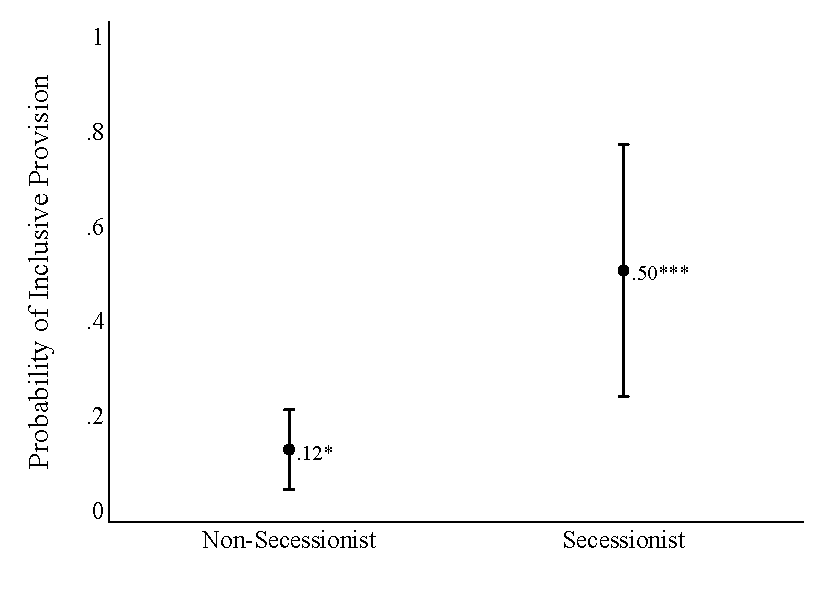
\includegraphics[width=\textwidth]{main.pdf}
    %\end{subfigure}
% 
%	\begin{subfigure}{0.45\textwidth}
%    \centering
%    \caption{Model 4, \autoref{table:mainint}} \label{figure:mainint}
%    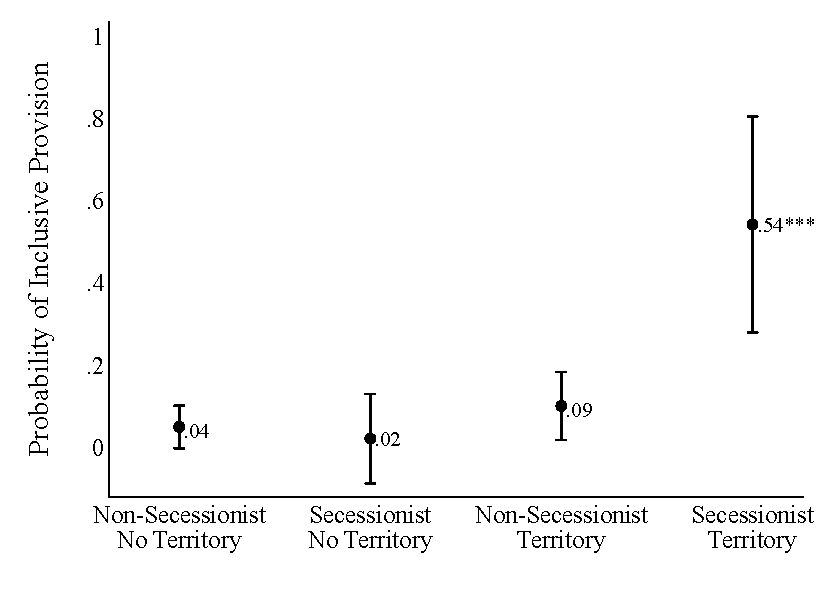
\includegraphics[width=\textwidth]{mainint.pdf}
%    \end{subfigure}
%  \begin{tablenotes}[para, flushleft]
%\raggedright \footnotesize{\textit{Note:} \autoref{figure:main} presents the predicted probability of \textit{Secessionist} rebel groups of providing inclusive services with all other variables set to their means. As is clear, secessionist rebel groups are between three to six times more likely to provide inclusive services than non-secessionist rebel groups. Moreover, the predicted effects of secessionist and non-secessionist goals on the probability of inclusive service provision is statistically significantly different (in \autoref{figure:mainc}: ${\chi^2}$= 5.00, $p<0.05$, and in \autoref{figure:mainint}: ${\chi^2}$= 7.94, $p<0.01$). Black vertical lines represent 90\% confidence intervals.}
%\end{tablenotes}
%\end{figure}



\begin{landscape}
\begin{table}[htbp]\centering
\begin{footnotesize}
\def\sym#1{\ifmmode^{#1}\else\(^{#1}\)\fi}
\newcounter{mym2}
\makeatletter
\def\myrow{}
\CT@everycr{\noalign{%
\global\let\CT@row@color\relax
\stepcounter{mym2}%
\ifnum\value{mym2}=2
  \gdef\myrow{\rowcolor{gray!50}}
\else\ifnum\value{mym2}=8
  \gdef\myrow{}
\fi\fi
}\myrow}
\renewcommand\thetable{A.\Roman{table}}
\caption{\textbf{Secessionism Predicts Inclusive Services, Interaction}}
\label{table:mainint}
\begin{tabular}{l*{8}{c}}
\hline\hline
                    &\multicolumn{1}{c}{(1)}&\multicolumn{1}{c}{(2)}&\multicolumn{1}{c}{(3)}&\multicolumn{1}{c}{(4)}&\multicolumn{1}{c}{(5)}&\multicolumn{1}{c}{(6)}&\multicolumn{1}{c}{(7)}&\multicolumn{1}{c}{(8)}\\
\hline
Secessionist $\times$ Territorial Control&        0.29\sym{**} &        0.32\sym{***}&        0.45\sym{**} &        0.47\sym{**} &        0.53\sym{***}&        0.57\sym{***}&        0.48\sym{+}  &        0.45\sym{**} \\
                    &      (0.12)         &      (0.12)         &      (0.18)         &      (0.19)         &      (0.20)         &      (0.19)         &      (0.32)         &      (0.20)         \\
Secessionist      &        0.05         &        0.02         &       -0.00         &       -0.03         &       -0.06         &       -0.09         &        0.22         &       -0.04         \\
                    &      (0.05)         &      (0.05)         &      (0.05)         &      (0.08)         &      (0.09)         &      (0.09)         &      (0.24)         &      (0.08)         \\
Territorial Control&        0.12\sym{**} &        0.09\sym{**} &        0.07\sym{*}  &        0.05         &        0.04         &        0.03         &       -0.08         &        0.06         \\
                    &      (0.05)         &      (0.04)         &      (0.04)         &      (0.05)         &      (0.05)         &      (0.06)         &      (0.09)         &      (0.05)         \\
Communist           &                     &       -0.01         &                     &       -0.09         &       -0.06         &       -0.06         &        0.16         &       -0.09         \\
                    &                     &      (0.05)         &                     &      (0.09)         &      (0.09)         &      (0.09)         &      (0.24)         &      (0.08)         \\
Ethnic War          &                     &        0.14\sym{+}  &                     &        0.03         &       -0.01         &       -0.03         &        0.23         &        0.05         \\
                    &                     &      (0.09)         &                     &      (0.10)         &      (0.10)         &      (0.11)         &      (0.28)         &      (0.09)         \\
Rebel Strength      &                     &       -0.02         &                     &       -0.01         &       -0.02         &       -0.02         &       -0.00         &       -0.02         \\
                    &                     &      (0.02)         &                     &      (0.04)         &      (0.04)         &      (0.04)         &      (0.04)         &      (0.04)         \\
Duration            &                     &        0.01\sym{***}&                     &        0.01\sym{*}  &        0.01\sym{*}  &        0.01\sym{*}  &        0.01\sym{+}  &        0.01\sym{*}  \\
                    &                     &      (0.00)         &                     &      (0.00)         &      (0.00)         &      (0.00)         &      (0.01)         &      (0.00)         \\
Infant Mortality    &                     &                     &        0.00         &        0.00         &        0.00         &        0.00\sym{+}  &        0.00         &        0.00         \\
                    &                     &                     &      (0.00)         &      (0.00)         &      (0.00)         &      (0.00)         &      (0.00)         &      (0.00)         \\
GDPpc               &                     &                     &        0.04\sym{+}  &        0.05\sym{+}  &        0.07\sym{*}  &        0.07\sym{**} &        0.08         &        0.07\sym{**} \\
                    &                     &                     &      (0.03)         &      (0.03)         &      (0.03)         &      (0.03)         &      (0.07)         &      (0.03)         \\
Democracy           &                     &                     &       -0.04         &       -0.06         &       -0.01         &        0.00         &        0.06         &       -0.08\sym{+}  \\
                    &                     &                     &      (0.06)         &      (0.06)         &      (0.07)         &      (0.06)         &      (0.06)         &      (0.05)         \\
Population (logged) &                     &                     &        0.01         &        0.01         &       -0.01         &       -0.01         &        0.06         &                     \\
                    &                     &                     &      (0.01)         &      (0.01)         &      (0.02)         &      (0.01)         &      (0.21)         &                     \\
Rugged Terrain      &                     &                     &        0.01         &        0.01         &        0.02         &        0.02         &        1.03         &                     \\
                    &                     &                     &      (0.02)         &      (0.03)         &      (0.02)         &      (0.02)         &      (0.83)         &                     \\
Competition         &                     &                     &                     &                     &                     &                     &                     &        0.01         \\
                    &                     &                     &                     &                     &                     &                     &                     &      (0.01)         \\
Population (change) &                     &                     &                     &                     &                     &                     &                     &        0.01         \\
                    &                     &                     &                     &                     &                     &                     &                     &      (0.01)         \\
Constant            &        0.05\sym{**} &       -0.00         &       -0.64\sym{*}  &       -0.60\sym{+}  &       -1.06\sym{***}&       -1.10\sym{***}&       -4.97\sym{**} &       -0.76\sym{**} \\
                    &      (0.02)         &      (0.03)         &      (0.36)         &      (0.40)         &      (0.32)         &      (0.33)         &      (2.31)         &      (0.35)         \\
\hline
Observations        &         254         &         253         &         177         &         176         &         176         &         176         &         176         &         165         \\
\(R^{2}\)           &       0.174         &       0.252         &       0.279         &       0.309         &       0.346         &       0.371         &       0.705         &       0.304         \\
\hline\hline
\multicolumn{9}{l}{\footnotesize Standard errors in parentheses. Standard errors clustered by country in all models.}\\
\multicolumn{9}{l}{\footnotesize \sym{+} \(p<0.15\), \sym{*} \(p<0.10\), \sym{**} \(p<0.05\), \sym{***} \(p<0.01\)}\\
\end{tabular}
\end{footnotesize}
\end{table}
\end{landscape}

\newpage
\begin{figure}[h]
\setcounter{figure}{0}
\renewcommand\thefigure{A.\arabic{figure}}
\caption{\textbf{Secessionist Coefficient Estimates}}
\label{figure:coef}
\centering
	\begin{subfigure}{0.45\textwidth}
    \centering
    \caption{\autoref{table:conditional}} \label{figure:coefmain}
    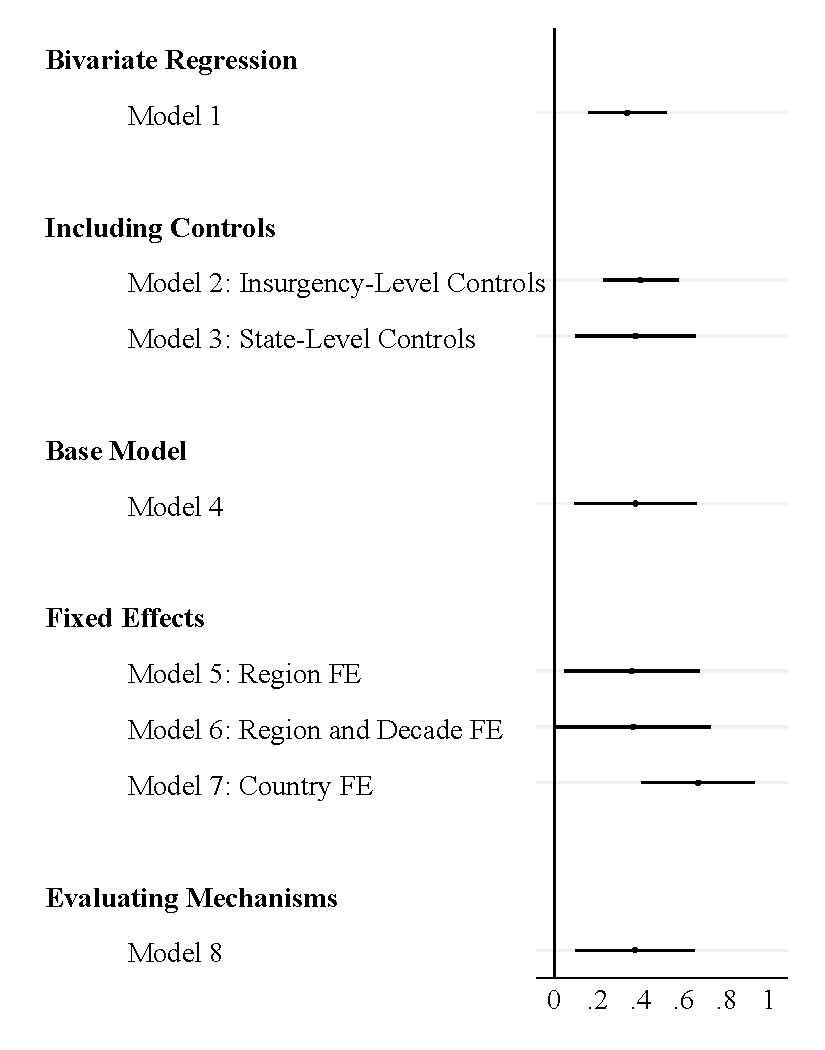
\includegraphics[width=\textwidth]{coefmain.pdf}
    \end{subfigure}
% 
	\begin{subfigure}{0.45\textwidth}
    \centering
    \caption{\autoref{table:mainint}} \label{figure:coefmainint}
    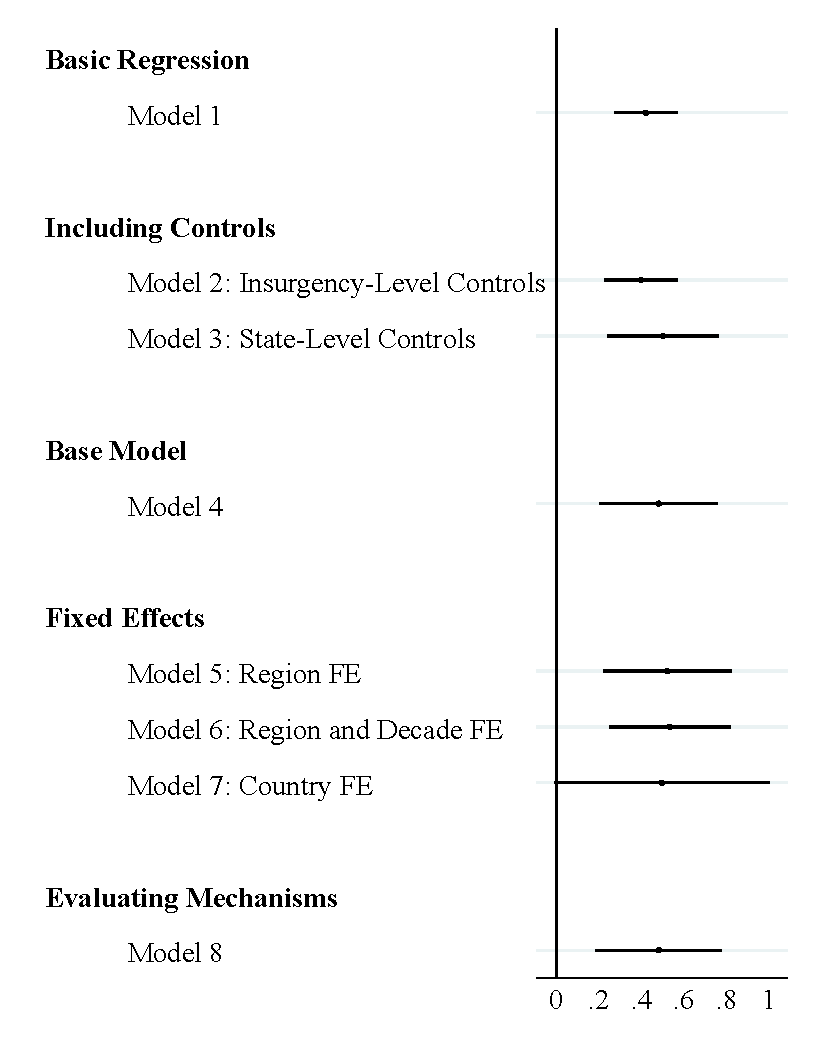
\includegraphics[width=\textwidth]{coefmainint.pdf}
    \end{subfigure}
  \begin{tablenotes}[para, flushleft]
\raggedright \footnotesize{\textit{Note:} \autoref{figure:coef} presents the coefficient estimates for the variable \textit{Secessionist} in \autoref{table:conditional} and \autoref{table:mainint}. Black horizontal lines represent 90\% confidence intervals. If the confidence intervals fail to overlap with the vertical black line, then the effect of \textit{Secessionist} is statistically significant. As can be seen, the results are highly similar, positive and robust across all specifications.}
\end{tablenotes}
\end{figure}

\newpage
\begin{figure}[h!]
\renewcommand\thefigure{A.\arabic{figure}}
\caption{\textbf{Predicted Effect of Secessionism on Inclusive Services}}
\label{figure:main}
\centering
	\begin{subfigure}{0.45\textwidth}
    \centering
    \caption{Model 4, \autoref{table:conditional}} \label{figure:mainc}
    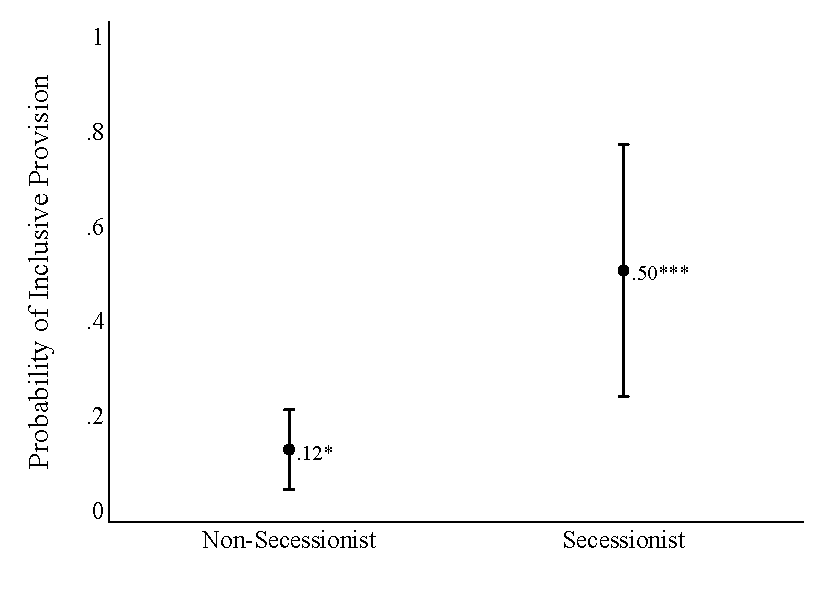
\includegraphics[width=\textwidth]{main.pdf}
    \end{subfigure}
% 
	\begin{subfigure}{0.45\textwidth}
    \centering
    \caption{Model 4, \autoref{table:mainint}} \label{figure:mainint}
    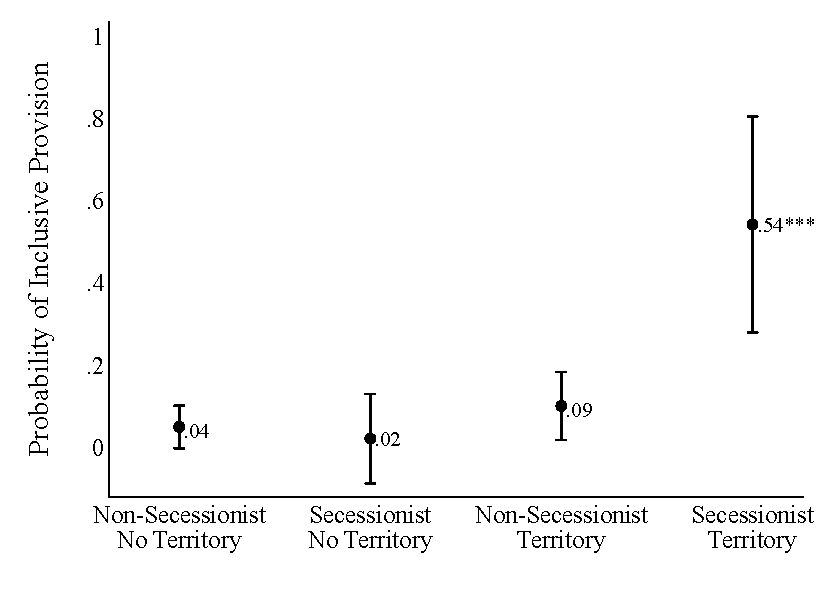
\includegraphics[width=\textwidth]{mainint.pdf}
    \end{subfigure}
  \begin{tablenotes}[para, flushleft]
\raggedright \footnotesize{\textit{Note:} \autoref{figure:main} presents the predicted probability of \textit{Secessionist} rebel groups of providing inclusive services with all other variables set to their means. As is clear, secessionist rebel groups are between three to six times more likely to provide inclusive services than non-secessionist rebel groups. Moreover, the predicted effects of secessionist and non-secessionist goals on the probability of inclusive service provision is statistically significantly different (in \autoref{figure:mainc}: ${\chi^2}$= 5.00, $p<0.05$, and in \autoref{figure:mainint}: ${\chi^2}$= 7.94, $p<0.01$). Black vertical lines represent 90\% confidence intervals.}
\end{tablenotes}
\end{figure}

\newpage
\begin{table}[htbp]\centering
\begin{small}
\def\sym#1{\ifmmode^{#1}\else\(^{#1}\)\fi}
\newcounter{mym3}
\makeatletter
\def\myrow{}
\CT@everycr{\noalign{%
\global\let\CT@row@color\relax
\stepcounter{mym3}%
\ifnum\value{mym3}=2
  \gdef\myrow{\rowcolor{gray!50}}
\else\ifnum\value{mym3}=4
  \gdef\myrow{}
\fi\fi
}\myrow}
\renewcommand\thetable{A.\Roman{table}}
\caption{\textbf{Additional Controls }}
\label{table:addcontrols1}
\begin{tabular}{l*{8}{c}}
\hline\hline
                    &\multicolumn{1}{c}{(1)}&\multicolumn{1}{c}{(2)}&\multicolumn{1}{c}{(3)}&\multicolumn{1}{c}{(4)}&\multicolumn{1}{c}{(5)}&\multicolumn{1}{c}{(6)}&\multicolumn{1}{c}{(7)}&\multicolumn{1}{c}{(8)}\\
\hline
Secessionist     &        0.37\sym{**} &        0.37\sym{**} &        0.35\sym{*}  &        0.34\sym{*}  &        0.38\sym{**} &        0.31\sym{*}  &        0.26         &        0.38\sym{**} \\
                    &      (0.17)         &      (0.17)         &      (0.17)         &      (0.19)         &      (0.15)         &      (0.17)         &      (0.20)         &      (0.17)         \\
Communist           &       -0.21         &       -0.19\sym{+}  &       -0.02         &       -0.18         &       -0.17         &       -0.12         &       -0.17         &       -0.17         \\
                    &      (0.16)         &      (0.12)         &      (0.13)         &      (0.15)         &      (0.16)         &      (0.15)         &      (0.14)         &      (0.17)         \\
Ethnic War          &        0.33         &        0.81\sym{***}&        0.36\sym{+}  &        0.42\sym{+}  &        0.42\sym{+}  &        0.49\sym{+}  &        0.48\sym{+}  &        0.43\sym{+}  \\
                    &      (0.25)         &      (0.16)         &      (0.24)         &      (0.29)         &      (0.28)         &      (0.29)         &      (0.29)         &      (0.27)         \\
Rebel Strength      &       -0.12\sym{*}  &       -0.10\sym{*}  &       -0.16\sym{*}  &       -0.06         &       -0.06         &       -0.05         &       -0.04         &                     \\
                    &      (0.06)         &      (0.05)         &      (0.09)         &      (0.06)         &      (0.06)         &      (0.06)         &      (0.06)         &                     \\
Duration            &        0.00         &       -0.00         &       -0.00         &        0.00         &        0.00         &        0.01         &        0.01         &        0.00         \\
                    &      (0.01)         &      (0.01)         &      (0.01)         &      (0.01)         &      (0.01)         &      (0.01)         &      (0.01)         &      (0.01)         \\
Infant Mortality    &        0.00         &        0.00\sym{+}  &        0.00         &        0.00         &        0.00         &        0.00         &        0.00         &        0.00         \\
                    &      (0.00)         &      (0.00)         &      (0.00)         &      (0.00)         &      (0.00)         &      (0.00)         &      (0.00)         &      (0.00)         \\
GDPpc               &        0.13\sym{*}  &        0.16\sym{*}  &        0.10         &        0.09         &        0.09         &        0.03         &        0.03         &        0.07         \\
                    &      (0.07)         &      (0.08)         &      (0.07)         &      (0.08)         &      (0.07)         &      (0.07)         &      (0.07)         &      (0.08)         \\
Democracy           &       -0.06         &       -0.04         &        0.12         &        0.00         &       -0.09         &       -0.04         &       -0.03         &       -0.02         \\
                    &      (0.18)         &      (0.14)         &      (0.17)         &      (0.17)         &      (0.13)         &      (0.12)         &      (0.13)         &      (0.16)         \\
Population (logged) &                     &        0.08         &        0.02         &        0.05         &        0.03         &        0.04         &        0.05         &        0.04         \\
                    &                     &      (0.05)         &      (0.05)         &      (0.05)         &      (0.04)         &      (0.04)         &      (0.04)         &      (0.05)         \\

Rugged Terrain      &        0.06         &        0.10\sym{**} &       -0.01         &        0.07         &        0.05         &        0.05         &        0.05         &        0.07         \\
                    &      (0.05)         &      (0.04)         &      (0.05)         &      (0.05)         &      (0.05)         &      (0.04)         &      (0.04)         &      (0.05)         \\
Population (change) &        0.04         &                     &                     &                     &                     &                     &                     &                     \\
                    &      (0.04)         &                     &                     &                     &                     &                     &                     &                     \\
Non-Military Aid    &                     &        0.27\sym{***}&                     &                     &                     &                     &                     &                     \\
                    &                     &      (0.09)         &                     &                     &                     &                     &                     &                     \\
Rebel Group Size    &                     &                     &        0.15\sym{**} &                     &                     &                     &                     &                     \\
                    &                     &                     &      (0.06)         &                     &                     &                     &                     &                     \\
Battle Deaths       &                     &                     &                     &       -0.00         &                     &                     &                     &                     \\
                    &                     &                     &                     &      (0.02)         &                     &                     &                     &                     \\
Competition         &                     &                     &                     &                     &        0.04\sym{*}  &                     &                     &                     \\
                    &                     &                     &                     &                     &      (0.03)         &                     &                     &                     \\
Pre-Conflict Education&                     &                     &                     &                     &                     &        0.35\sym{*}  &                     &                     \\
                    &                     &                     &                     &                     &                     &      (0.19)         &                     &                     \\
Pre-Conflict Health &                     &                     &                     &                     &                     &                     &        0.33\sym{*}  &                     \\
                    &                     &                     &                     &                     &                     &                     &      (0.19)         &                     \\
Rebel Strength Categories      &                     &                     &                     &                     &                     &                     &                     &        Yes         \\
                    &                     &                     &                     &                     &                     &                     &                     &               \\
Constant            &       -1.56\sym{+}  &       -2.70\sym{*}  &       -2.15\sym{+}  &       -1.57         &       -1.40         &       -0.95         &       -1.14         &       -1.43         \\
                    &      (0.99)         &      (1.45)         &      (1.28)         &      (1.52)         &      (1.23)         &      (1.04)         &      (1.06)         &      (1.46)         \\
\hline
Observations        &          51         &          49         &          51         &          53         &          56         &          54         &          54         &          56         \\
\(R^{2}\)           &       0.390         &       0.494         &       0.436         &       0.341         &       0.404         &       0.452         &       0.445         &       0.371         \\
\hline\hline
\multicolumn{9}{l}{\footnotesize Standard errors in parentheses.}\\
\multicolumn{9}{l}{\footnotesize Standard errors clustered by country in all models.}\\
\multicolumn{9}{l}{\footnotesize \sym{+} \(p<0.15\), \sym{*} \(p<0.10\), \sym{**} \(p<0.05\), \sym{***} \(p<0.01\)}\\
\end{tabular}
\end{small}
\end{table}

\newpage
\begin{table}[htbp]\centering
\begin{small}
\def\sym#1{\ifmmode^{#1}\else\(^{#1}\)\fi}
\setcounter{table}{5}
\newcounter{mym4}
\makeatletter
\def\myrow{}
\CT@everycr{\noalign{%
\global\let\CT@row@color\relax
\stepcounter{mym4}%
\ifnum\value{mym4}=2
  \gdef\myrow{\rowcolor{gray!50}}
\else\ifnum\value{mym4}=4
  \gdef\myrow{}
\fi\fi
}\myrow}
\renewcommand\thetable{A.\Roman{table}}
\caption{\textbf{Additional Controls, Cont.}}
\label{table:addcontrols2}
\begin{tabular}{l*{4}{c}}
\hline\hline
                    &\multicolumn{1}{c}{(9)}&\multicolumn{1}{c}{(10)}&\multicolumn{1}{c}{(11)}&\multicolumn{1}{c}{(12)}\\
\hline
Secessionist      &        0.45\sym{**} &        0.51\sym{**} &        0.45\sym{**} &        0.54\sym{**} \\
                    &      (0.20)         &      (0.20)         &      (0.18)         &      (0.21)         \\
Communist           &        0.03         &        0.01         &        0.21         &        0.26         \\
                    &      (0.19)         &      (0.24)         &      (0.19)         &      (0.18)         \\
Ethnic War          &        0.29         &        0.30         &        0.54         &        0.43         \\
                    &      (0.44)         &      (0.37)         &      (0.44)         &      (0.52)         \\
Duration            &        0.00         &       -0.00         &       -0.01         &       -0.00         \\
                    &      (0.01)         &      (0.01)         &      (0.01)         &      (0.01)         \\
Infant Mortality    &        0.00         &        0.00         &       -0.00         &       -0.00         \\
                    &      (0.00)         &      (0.00)         &      (0.00)         &      (0.00)         \\
GDPpc               &       -0.00         &       -0.01         &        0.11         &        0.13         \\
                    &      (0.10)         &      (0.13)         &      (0.09)         &      (0.11)         \\
Democracy           &        0.01         &        0.09         &        0.07         &        0.12         \\
                    &      (0.15)         &      (0.15)         &      (0.18)         &      (0.21)         \\
Population (logged) &       -0.06         &                     &       -0.02         &       -0.04         \\
                    &      (0.07)         &                     &      (0.07)         &      (0.07)         \\
Rugged Terrain      &       -0.04         &       -0.05         &        0.03         &       -0.01         \\
                    &      (0.08)         &      (0.07)         &      (0.07)         &      (0.10)         \\
Population (change) &                     &       -0.07         &                     &                     \\
                    &                     &      (0.07)         &                     &                     \\
Non-Military Aid    &        0.06         &        0.12         &        0.05         &       -0.07         \\
                    &      (0.18)         &      (0.14)         &      (0.15)         &      (0.19)         \\
Rebel Group Size    &        0.29\sym{**} &        0.33\sym{***}&        0.34\sym{**} &        0.42\sym{***}\\
                    &      (0.13)         &      (0.09)         &      (0.13)         &      (0.15)         \\
Competition         &        0.01         &       -0.01         &        0.00         &        0.00         \\
                    &      (0.02)         &      (0.03)         &      (0.03)         &      (0.05)         \\
Battle Deaths       &       -0.08\sym{*}  &       -0.10\sym{**} &       -0.07\sym{**} &       -0.06\sym{*}  \\
                    &      (0.04)         &      (0.04)         &      (0.03)         &      (0.03)         \\
Pre-Conflict Education&        0.40         &        0.24         &        0.73\sym{**} &        0.76\sym{**} \\
                    &      (0.28)         &      (0.27)         &      (0.28)         &      (0.33)         \\
Pre-Conflict Health &       -0.14         &        0.03         &       -0.38\sym{+}  &       -0.41\sym{+}  \\
                    &      (0.23)         &      (0.23)         &      (0.24)         &      (0.26)         \\
Rebel Strength Categories      &         Yes  &         Yes &       Yes &       Yes  \\
                    &          &              &               &               \\
Constant            &       -1.47         &       -1.57         &       -3.06\sym{**} &       -3.14\sym{**} \\
                    &      (1.44)         &      (1.74)         &      (1.29)         &      (1.35)         \\
\\
Region Fixed Effects               &      No               &         No            &         Yes            &      Yes     \\
Decade Fixed Effects               &      No               &         No            &         No            &      Yes     \\                    
\hline
Observations        &          42         &          39         &          42         &          42         \\
\(R^{2}\)           &       0.721         &       0.754         &       0.831         &       0.861         \\
\hline\hline
\multicolumn{5}{l}{\footnotesize Standard errors in parentheses.}\\
\multicolumn{5}{l}{\footnotesize Standard errors clustered by country in all models.}\\
\multicolumn{5}{l}{\footnotesize \sym{+} \(p<0.15\), \sym{*} \(p<0.10\), \sym{**} \(p<0.05\), \sym{***} \(p<0.01\)}\\
\end{tabular}
\end{small}
\end{table}


\newpage
\begin{table}[htbp]\centering
\begin{small}
\def\sym#1{\ifmmode^{#1}\else\(^{#1}\)\fi}
\renewcommand\thetable{A.\Roman{table}}
\newcounter{mym5}
\makeatletter
\def\myrow{}
\CT@everycr{\noalign{%
\global\let\CT@row@color\relax
\stepcounter{mym5}%
\ifnum\value{mym5}=2
  \gdef\myrow{\rowcolor{gray!50}}
\else\ifnum\value{mym5}=4
  \gdef\myrow{}
\fi\fi
}\myrow}
\caption{\textbf{Excluding Outliers }}
\label{table:outliers}
\begin{tabular}{l*{1}{c}}
\hline\hline
                    &\multicolumn{1}{c}{(1)}\\
\hline
Secessionist      &        0.48\sym{***}\\
                    &      (0.13)         \\
Communist           &       -0.20\sym{+}  \\
                    &      (0.13)         \\
Ethnic War          &        0.00         \\
                    &         (.)         \\
Rebel Strength      &       -0.05         \\
                    &      (0.05)         \\
Duration            &        0.00         \\
                    &      (0.01)         \\
Infant Mortality    &        0.00\sym{***}\\
                    &      (0.00)         \\
GDPpc               &        0.12\sym{***}\\
                    &      (0.04)         \\
Democracy           &       -0.07         \\
                    &      (0.13)         \\
Population (logged) &        0.08\sym{*}  \\
                    &      (0.04)         \\
Rugged Terrain      &        0.10\sym{***}\\
                    &      (0.03)         \\
Constant            &       -2.63\sym{**} \\
                    &      (0.98)         \\
\hline
Observations        &          49         \\
\(R^{2}\)           &       0.602         \\
\hline\hline
\multicolumn{2}{l}{\footnotesize Standard errors in parentheses.}\\
\multicolumn{2}{l}{\footnotesize Standard errors clustered by country in all models.}\\
\multicolumn{2}{l}{\footnotesize \sym{+} \(p<0.15\), \sym{*} \(p<0.10\), \sym{**} \(p<0.05\), \sym{***} \(p<0.01\)}\\
\end{tabular}
\end{small}
\end{table}


\newpage
\begin{table}[htbp]\centering
\def\sym#1{\ifmmode^{#1}\else\(^{#1}\)\fi}
\renewcommand\thetable{A.\Roman{table}}
\newcounter{mym6}
\makeatletter
\def\myrow{}
\CT@everycr{\noalign{%
\global\let\CT@row@color\relax
\stepcounter{mym6}%
\ifnum\value{mym6}=2
  \gdef\myrow{\rowcolor{gray!50}}
\else\ifnum\value{mym6}=4
  \gdef\myrow{}
\fi\fi
}\myrow}
\begin{small}
\caption{\textbf{Jackknifing }}
\label{table:jackknife}
\begin{tabular}{l*{1}{c}}
\hline\hline
                    &\multicolumn{1}{c}{(1)}\\
\hline
Secessionist      &        0.38\sym{**} \\
                    &      (0.18)         \\
Communist           &       -0.17         \\
                    &      (0.15)         \\
Ethnic War          &        0.42         \\
                    &      (0.51)         \\
Rebel Strength      &       -0.08         \\
                    &      (0.07)         \\
Duration            &        0.00         \\
                    &      (0.01)         \\
Infant Mortality    &        0.00         \\
                    &      (0.00)         \\
GDPpc               &        0.08         \\
                    &      (0.09)         \\
Democracy           &       -0.01         \\
                    &      (0.18)         \\
Population (logged) &        0.05         \\
                    &      (0.06)         \\
Rugged Terrain      &        0.06         \\
                    &      (0.05)         \\
Constant            &       -1.44         \\
                    &      (1.62)         \\
\hline
Observations        &          56         \\
\(R^{2}\)           &       0.365         \\
\hline\hline
\multicolumn{2}{l}{\footnotesize Standard errors in parentheses.}\\
\multicolumn{2}{l}{\footnotesize \sym{+} \(p<0.15\), \sym{*} \(p<0.10\), \sym{**} \(p<0.05\), \sym{***} \(p<0.01\)}\\
\end{tabular}
\end{small}
\end{table}

\newpage
\begin{table}[htbp]\centering
\def\sym#1{\ifmmode^{#1}\else\(^{#1}\)\fi}
\begin{small}
\renewcommand\thetable{A.\Roman{table}}
\newcounter{mym7}
\makeatletter
\def\myrow{}
\CT@everycr{\noalign{%
\global\let\CT@row@color\relax
\stepcounter{mym7}%
\ifnum\value{mym7}=2
  \gdef\myrow{\rowcolor{gray!50}}
\else\ifnum\value{mym7}=4
  \gdef\myrow{}
\fi\fi
}\myrow}
\caption{\textbf{Original Dataset}}
\label{table:original}
\begin{tabular}{l*{1}{c}}
\hline\hline
                    &\multicolumn{1}{c}{(1)}\\
\hline
Secessionist       &        0.36\sym{**} \\
                    &      (0.17)         \\
Communist     &       -0.20         \\
                    &      (0.17)         \\
Ethnic War           &        0.35         \\
                    &      (0.28)         \\
Rebel Strength        &       -0.11\sym{+}  \\
                    &      (0.07)         \\
Duration                 &        0.00         \\
                    &      (0.01)         \\
Infant Mortality        &        0.00         \\
                    &      (0.00)         \\
GDPpc      &        0.11         \\
                    &      (0.08)         \\
Democracy   &        0.06         \\
                    &      (0.18)         \\
Total Population   &        0.03         \\
                    &      (0.05)         \\
Rugged Terrain       &        0.05         \\
                    &      (0.04)         \\
Constant            &       -1.33         \\
                    &      (1.36)         \\
\hline
Observations        &          57         \\
\(R^{2}\)           &       0.343         \\
\hline\hline
\multicolumn{2}{l}{\footnotesize Standard errors in parentheses}\\
\multicolumn{2}{l}{\footnotesize Standard errors clustered by country in all models.}\\
\multicolumn{2}{l}{\footnotesize \sym{+} \(p<0.15\), \sym{*} \(p<0.10\), \sym{**} \(p<0.05\), \sym{***} \(p<0.01\)}\\
\end{tabular}
\end{small}
\end{table}

\newpage
\begin{table}[htbp]\centering
\begin{small}
\def\sym#1{\ifmmode^{#1}\else\(^{#1}\)\fi}
\renewcommand\thetable{A.\Roman{table}}
\caption{\textbf{Correcting for Information Bias }}
\newcounter{mym8}
\makeatletter
\def\myrow{}
\CT@everycr{\noalign{%
\global\let\CT@row@color\relax
\stepcounter{mym8}%
\ifnum\value{mym8}=4
  \gdef\myrow{\rowcolor{gray!50}}
\else\ifnum\value{mym8}=6
  \gdef\myrow{}
\fi\fi
}\myrow}
\renewcommand\thetable{A.\Roman{table}}
\label{table:info}
\begin{tabular}{l*{3}{c}}
\hline\hline
 &\multicolumn{1}{c}{(1)}&\multicolumn{1}{c}{(2)}&\multicolumn{1}{c}{(3)}\\
                    &\multicolumn{1}{c}{Large}&\multicolumn{1}{c}{Post-1970}&\multicolumn{1}{c}{No Missingness,}\\
  &\multicolumn{1}{c}{Insurgencies}&\multicolumn{1}{c}{Insurgencies}&\multicolumn{1}{c}{No Services}\\
  \hline
Secessionist      &        0.56\sym{**} &        0.35\sym{**} &        0.33\sym{**} \\
                    &      (0.25)         &      (0.17)         &      (0.15)         \\
Rebel Strength      &       -0.05         &       -0.12\sym{*}  &       -0.08\sym{+}  \\
                    &      (0.10)         &      (0.07)         &      (0.05)         \\
Communist           &       -0.03         &       -0.22\sym{+}  &       -0.17         \\
                    &      (0.45)         &      (0.13)         &      (0.14)         \\
Ethnic War          &        0.82\sym{**} &        0.37\sym{*}  &        0.43\sym{+}  \\
                    &      (0.38)         &      (0.21)         &      (0.27)         \\
Duration            &        0.01         &        0.01         &        0.00         \\
                    &      (0.02)         &      (0.01)         &      (0.01)         \\
Infant Mortality    &       -0.00         &        0.00         &        0.00         \\
                    &      (0.00)         &      (0.00)         &      (0.00)         \\
GDPpc               &       -0.07         &        0.07         &        0.07         \\
                    &      (0.13)         &      (0.08)         &      (0.06)         \\
Population (logged) &       -0.07         &        0.04         &        0.04         \\
                    &      (0.11)         &      (0.05)         &      (0.04)         \\
Democracy           &       -0.19         &        0.04         &       -0.04         \\
                    &      (0.20)         &      (0.16)         &      (0.13)         \\
Rugged Terrain      &        0.02         &        0.07\sym{+}  &        0.06\sym{*}  \\
                    &      (0.08)         &      (0.04)         &      (0.03)         \\
Constant            &        1.84         &       -1.20         &       -1.29         \\
                    &      (2.67)         &      (1.44)         &      (0.97)         \\
\hline
Observations        &          31         &          52         &          62         \\
\(R^{2}\)           &       0.384         &       0.429         &       0.332         \\
\hline\hline
\multicolumn{4}{l}{\footnotesize Standard errors in parentheses.}\\
\multicolumn{4}{l}{\footnotesize Standard errors clustered by country in all models.}\\
\multicolumn{4}{l}{\footnotesize \sym{+} \(p<0.15\), \sym{*} \(p<0.10\), \sym{**} \(p<0.05\), \sym{***} \(p<0.01\)}\\
\end{tabular}
\end{small}
\end{table}



\newpage
\begin{table}[htbp]\centering
\begin{small}
\def\sym#1{\ifmmode^{#1}\else\(^{#1}\)\fi}
\renewcommand\thetable{A.\Roman{table}}
\caption{\textbf{Alternative Secessionist Specification }}
\newcounter{mym9}
\makeatletter
\def\myrow{}
\CT@everycr{\noalign{%
\global\let\CT@row@color\relax
\stepcounter{mym9}%
\ifnum\value{mym9}=2
  \gdef\myrow{\rowcolor{gray!50}}
\else\ifnum\value{mym9}=8
  \gdef\myrow{}
\fi\fi
}\myrow}
\label{table:altsec}
\begin{tabular}{l*{3}{c}}
\hline\hline
                    &\multicolumn{1}{c}{(1)}&\multicolumn{1}{c}{(2)}&\multicolumn{1}{c}{(3)}\\
\hline
Secessionist (Broadly Defined)&        0.38\sym{**} &                     &                     \\
                    &      (0.17)         &                     &                     \\
Secessionist (Broadly Defined)&                     &        0.42\sym{**} &                     \\
                    &                     &      (0.15)         &                     \\
Secessionist (Broadly Defined)&                     &                     &        0.45\sym{***}\\
                    &                     &                     &      (0.15)         \\
Communist           &       -0.17         &       -0.14         &       -0.11         \\
                    &      (0.15)         &      (0.15)         &      (0.15)         \\
Ethnic War          &        0.42\sym{+}  &        0.49\sym{*}  &        0.28\sym{+}  \\
                    &      (0.27)         &      (0.29)         &      (0.16)         \\
Rebel Strength      &       -0.08         &       -0.06         &       -0.05         \\
                    &      (0.06)         &      (0.06)         &      (0.06)         \\
Duration            &        0.00         &        0.00         &        0.00         \\
                    &      (0.01)         &      (0.01)         &      (0.01)         \\
Infant Mortality    &        0.00         &        0.00         &        0.00         \\
                    &      (0.00)         &      (0.00)         &      (0.00)         \\
GDPpc               &        0.08         &        0.06         &        0.05         \\
                    &      (0.07)         &      (0.07)         &      (0.07)         \\
Democracy           &       -0.01         &       -0.07         &       -0.06         \\
                    &      (0.17)         &      (0.16)         &      (0.16)         \\
Population (logged) &        0.05         &        0.05         &        0.04         \\
                    &      (0.05)         &      (0.05)         &      (0.05)         \\
Rugged Terrain      &        0.06         &        0.07\sym{+}  &        0.07\sym{+}  \\
                    &      (0.04)         &      (0.04)         &      (0.04)         \\
Constant            &       -1.44         &       -1.44         &       -1.23         \\
                    &      (1.38)         &      (1.35)         &      (1.35)         \\
\hline
Observations        &          56         &          56         &          56         \\
\(R^{2}\)           &       0.365         &       0.401         &       0.422         \\
\hline\hline
\multicolumn{4}{l}{\footnotesize Standard errors in parentheses.}\\
\multicolumn{4}{l}{\footnotesize Standard errors clustered by country in all models.}\\
\multicolumn{4}{l}{\footnotesize \sym{+} \(p<0.15\), \sym{*} \(p<0.10\), \sym{**} \(p<0.05\), \sym{***} \(p<0.01\)}\\
\end{tabular}
\end{small}
\end{table}

\newpage
\begin{table}[htbp]\centering
\begin{small}
\def\sym#1{\ifmmode^{#1}\else\(^{#1}\)\fi}
\renewcommand\thetable{A.\Roman{table}}
\newcounter{mym10}
\makeatletter
\def\myrow{}
\CT@everycr{\noalign{%
\global\let\CT@row@color\relax
\stepcounter{mym10}%
\ifnum\value{mym10}=3
  \gdef\myrow{\rowcolor{gray!50}}
\else\ifnum\value{mym10}=5
  \gdef\myrow{}
\fi\fi
}\myrow}
\caption{\textbf{Alternative Inclusive Services Specification}}
\label{table:altpg}
\begin{tabular}{l*{3}{c}}
\hline\hline
                    &\multicolumn{1}{c}{(1)}&\multicolumn{1}{c}{(2)}&\multicolumn{1}{c}{(3)}\\
                    &\multicolumn{1}{c}{Any Inclusive Services}&\multicolumn{1}{c}{Alternative Coding}&\multicolumn{1}{c}{Ordinal Ranking}\\
\hline
Secessionist      &        0.42\sym{**} &        0.36\sym{**} &        0.55\sym{**} \\
                    &      (0.18)         &      (0.17)         &      (0.23)         \\
Communist           &        0.04         &       -0.15         &       -0.02         \\
                    &      (0.18)         &      (0.17)         &      (0.28)         \\
Ethnic War          &        0.39         &        0.27         &        0.24         \\
                    &      (0.30)         &      (0.29)         &      (0.62)         \\
Rebel Strength      &       -0.04         &       -0.14\sym{*}  &       -0.10         \\
                    &      (0.06)         &      (0.07)         &      (0.12)         \\
Duration            &       -0.00         &        0.00         &        0.01         \\
                    &      (0.01)         &      (0.01)         &      (0.01)         \\
Infant Mortality    &       -0.00         &        0.00\sym{+}  &        0.00         \\
                    &      (0.00)         &      (0.00)         &      (0.00)         \\
GDPpc               &        0.09         &        0.18\sym{*}  &        0.18\sym{+}  \\
                    &      (0.08)         &      (0.09)         &      (0.12)         \\
Democracy           &        0.07         &        0.02         &        0.22         \\
                    &      (0.19)         &      (0.17)         &      (0.25)         \\
Population (logged) &        0.06         &        0.01         &        0.02         \\
                    &      (0.05)         &      (0.05)         &      (0.08)         \\
Rugged Terrain      &       -0.00         &        0.05         &        0.08         \\
                    &      (0.05)         &      (0.05)         &      (0.08)         \\
Constant            &       -1.36         &       -1.59         &       -1.38         \\
                    &      (1.36)         &      (1.37)         &      (2.23)         \\
\hline
Observations        &          57         &          57         &          57         \\
\(R^{2}\)           &       0.382         &       0.334         &       0.301         \\
\hline\hline
\multicolumn{3}{l}{\footnotesize Standard errors in parentheses.}\\
\multicolumn{3}{l}{\footnotesize Standard errors clustered by country in all models.}\\
\multicolumn{3}{l}{\footnotesize \sym{+} \(p<0.15\), \sym{*} \(p<0.10\), \sym{**} \(p<0.05\), \sym{***} \(p<0.01\)}\\\
\end{tabular}
\end{small}
\end{table}

\newpage
\begin{table}[htbp]\centering
\begin{small}
\def\sym#1{\ifmmode^{#1}\else\(^{#1}\)\fi}
\renewcommand\thetable{A.\Roman{table}}
\newcounter{mym11}
\makeatletter
\def\myrow{}
\CT@everycr{\noalign{%
\global\let\CT@row@color\relax
\stepcounter{mym11}%
\ifnum\value{mym11}=3
  \gdef\myrow{\rowcolor{gray!50}}
\else\ifnum\value{mym11}=5
  \gdef\myrow{}
\fi\fi
}\myrow}
\caption{\textbf{Alternative Estimator }}
\label{table:altest}
\begin{tabular}{l*{2}{c}}
\hline\hline\
                    &\multicolumn{1}{c}{(1)}&\multicolumn{1}{c}{(2)}\\
                    &\multicolumn{1}{c}{Logit}&\multicolumn{1}{c}{Ordered Logit}\\
\hline
Secessionist      &        2.49\sym{**} &        1.95\sym{**} \\
                    &      (0.97)         &      (0.95)         \\
Communist           &       -1.68         &       -0.17         \\
                    &      (1.64)         &      (0.86)         \\
Ethnic War          &        2.42\sym{*}  &        0.85         \\
                    &      (1.33)         &      (1.94)         \\
Rebel Strength      &       -1.11\sym{*}  &       -0.30         \\
                    &      (0.64)         &      (0.37)         \\
Duration            &        0.03         &        0.04         \\
                    &      (0.07)         &      (0.04)         \\
Infant Mortality    &        0.01         &        0.01         \\
                    &      (0.02)         &      (0.01)         \\
GDPpc               &        0.56         &        0.73\sym{*}  \\
                    &      (0.64)         &      (0.44)         \\
Democracy           &       -0.23         &        0.58         \\
                    &      (1.20)         &      (0.68)         \\
Population (logged) &        0.09         &        0.15         \\
                    &      (0.28)         &      (0.29)         \\
Rugged Terrain      &        0.71\sym{*}  &        0.26         \\
                    &      (0.37)         &      (0.25)         \\
Constant            &       -9.31         &                     \\
                    &      (7.64)         &                     \\
\hline
cut1                &                     &                     \\
Constant            &                     &        9.01         \\
                    &                     &      (8.27)         \\
\hline
cut2                &                     &                     \\
Constant            &                     &       11.81         \\
                    &                     &      (8.70)         \\
\hline
Observations        &          56         &          57         \\
Pseudo \(R^{2}\)           &     0.362                &   0.175                  \\
\hline\hline
\multicolumn{3}{l}{\footnotesize Standard errors in parentheses}\\
\multicolumn{3}{l}{\footnotesize Standard errors clustered by country.}\\
\multicolumn{3}{l}{\footnotesize \sym{+} \(p<0.15\), \sym{*} \(p<0.10\), \sym{**} \(p<0.05\), \sym{***} \(p<0.01\)}\\
\end{tabular}
\end{small}
\end{table}

\newpage
\begin{table}[htbp]\centering
\begin{small}
\def\sym#1{\ifmmode^{#1}\else\(^{#1}\)\fi}
\renewcommand\thetable{A.\Roman{table}}
\newcounter{mym224}
\makeatletter
\def\myrow{}
\CT@everycr{\noalign{%
\global\let\CT@row@color\relax
\stepcounter{mym224}%
\ifnum\value{mym224}=3
  \gdef\myrow{\rowcolor{gray!50}}
\else\ifnum\value{mym224}=5
  \gdef\myrow{}
\fi\fi
}\myrow}
\caption{\textbf{Multiple Imputation}}
\label{table:micec}
\begin{tabular}{l*{1}{c}}
\hline\hline
                    &\multicolumn{1}{c}{(1)}\\
                    &\multicolumn{1}{c}{Public Goods}\\
\hline
Secessionist        &        0.38\sym{***}\\
                    &      (0.13)         \\
Communist           &        0.07         \\
                    &      (0.12)         \\
Ethnic War          &        0.51\sym{***}\\
                    &      (0.18)         \\
Rebel Strength      &       -0.02         \\
                    &      (0.06)         \\
Duration            &        0.01         \\
                    &      (0.01)         \\
Infant Mortality    &       -0.00         \\
                    &      (0.00)         \\
GDPpc               &        0.02         \\
                    &      (0.08)         \\
Democracy           &       -0.06         \\
                    &      (0.12)         \\
Population (logged) &        0.02         \\
                    &      (0.04)         \\
Rugged Terrain      &        0.02         \\
                    &      (0.04)         \\
\hline
Observations        &          92         \\
\hline\hline
\multicolumn{2}{l}{\footnotesize Standard errors in parentheses.}\\
\multicolumn{2}{l}{\footnotesize Standard errors clustered by country in all models.}\\
\multicolumn{2}{l}{\footnotesize \sym{+} \(p<0.15\), \sym{*} \(p<0.10\), \sym{**} \(p<0.05\), \sym{***} \(p<0.01\)}\\
\end{tabular}
\end{small}
\end{table}



\newpage
\clearpage
\begin{center}
\Large{\textbf{Appendix 4: Model Accuracy Diagnostics}}
\end{center}

In Table \ref{table:mainint}, I use the full sample of insurgencies to evaluate whether the interaction of \textit{Secessionist $\times$ Territorial Control} predicts rebel inclusive service provision. I conduct a joint significance test to ensure that the interaction of \textit{Secessionist $\times$ Territorial Control} and the coefficients of its lower-order terms are statistically different from the coefficient \textit{Secessionist}. The chi-square value is 4.92, indicating the coefficients are significantly different from each other at the 95\% level.

To assess the predictive power of the model, I present a Receiver Operator Characteristic (ROC) plot (Figure \ref{figure:roccurve}). The ROC plot illustrates the relationship between the rate of false positives and the rate of true positives, or how well a model is able to correctly predict inclusive service provision relative to incorrectly predicting inclusive service provision.\footnote{\citealt{ward2010perils, young2012repression}} The greater the Area Under the Curve (AUC), the greater predictive accuracy the model has. To ascertain the predictive accuracy of the model, I re-analyze Model 4 of \autoref{table:conditional} but use logistic regression. The AUC is 0.89/1.00, indicating that the model correctly predicts 89\% of cases. Moreover, the \textit{Secessionist} variable has the greatest predictive accuracy in comparison to all other variables (the AUC is 0.69/1.00). As a point of comparison, I determine the AUC of Model 4 of \autoref{table:mainint}, analyzed using logistic regression, and present the results in \autoref{figure:roccurve2}. Again, the AUC is extremely high at 0.90/1.00.


%When excluding the interaction term and its lower-order terms from the model, the AUC is just 0.73/1.00. As a comparison, the AUC of the model with simply the interaction term and lower-order terms is 0.72/1.00, suggesting that the interaction term alone predicts outcomes correctly at almost the same rate as all other control variables combined.


To assess the model's ability to predict future response cases, I re-estimate Model 4 of Table \ref{table:conditional} using a bootstrapping technique of sampling with replacement. The bootstrapping technique involves creating a sub-sample of data whereby observations have an equal probability of being selected for the sample, and the same observations may be included multiple times in the sub-sample \citep{efron1983leisurely, efron1997improvements}. The model is re-estimated multiple times using this limited sample, and the coefficients and standard errors are re-calculated. In this case, I set the sub-sample size to 30 observations, about one-third of the number of insurgencies that control territory. I then replicate the model 500 times. The results are robust, indicating that the model would perform well in its ability to predict future out-of-sample cases (Appendix Table \ref{table:boot}).

\newpage
\begin{figure}[h]
\renewcommand\thefigure{A.\arabic{figure}}
\caption{\textbf{ROC Curves of Predicted Accuracy}}
\label{figure:roccurve}
\centering
	\begin{subfigure}{0.45\textwidth}
    \centering
    \caption{Model 4, \autoref{table:conditional}} \label{figure:roccurve1}
    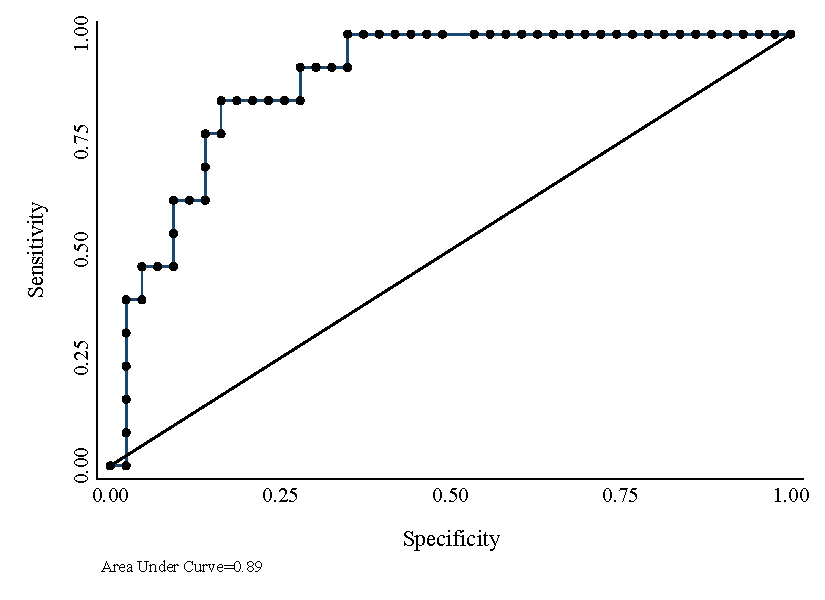
\includegraphics[width=\textwidth]{roccurve1.pdf}
    \end{subfigure}
% 
	\begin{subfigure}{0.45\textwidth}
    \centering
    \caption{Model 4, \autoref{table:mainint}} \label{figure:roccurve2}
    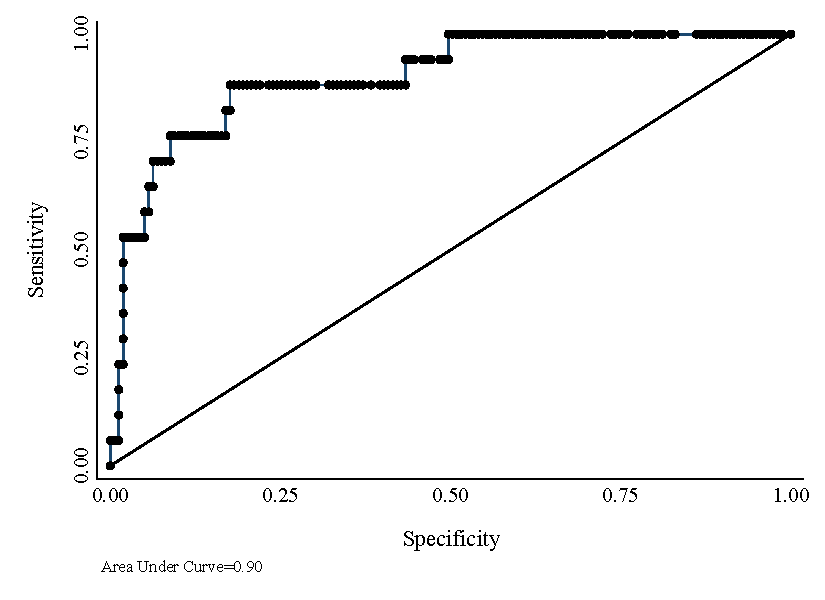
\includegraphics[width=\textwidth]{roccurve2.pdf}
    \end{subfigure}
  \begin{tablenotes}[para, flushleft]
\raggedright \footnotesize{\textit{Note:} The figure demonstrates the predictive power of Model 4 in  \autoref{table:conditional}. The AUC for Model 4, \autoref{table:conditional} is 0.89 and the AUC for Model 4, \autoref{table:mainint} is .90 meaning that the model is highly capable of correctly predicting insurgencies likely to provide inclusive services.}
\end{tablenotes}
\end{figure}

\newpage
\begin{table}[htbp]\centering
\begin{small}
\def\sym#1{\ifmmode^{#1}\else\(^{#1}\)\fi}
\renewcommand\thetable{A.\Roman{table}}
\newcounter{mym12}
\makeatletter
\def\myrow{}
\CT@everycr{\noalign{%
\global\let\CT@row@color\relax
\stepcounter{mym12}%
\ifnum\value{mym12}=2
  \gdef\myrow{\rowcolor{gray!50}}
\else\ifnum\value{mym12}=4
  \gdef\myrow{}
\fi\fi
}\myrow}
\caption{\textbf{Bootstrapping }}
\label{table:boot}
\begin{tabular}{l*{1}{c}}
\hline\hline
                    &\multicolumn{1}{c}{(1)}\\
\hline
Secessionist     &        0.38\sym{*}  \\
                    &      (0.22)         \\
Communist           &       -0.17         \\
                    &      (0.20)         \\
Ethnic War          &        0.42         \\
                    &      (0.36)         \\
Rebel Strength      &       -0.08         \\
                    &      (0.08)         \\
Duration            &        0.00         \\
                    &      (0.01)         \\
Infant Mortality    &        0.00         \\
                    &      (0.00)         \\
GDPpc               &        0.08         \\
                    &      (0.11)         \\
Democracy           &       -0.01         \\
                    &      (0.26)         \\
Population (logged) &        0.05         \\
                    &      (0.07)         \\
Rugged Terrain      &        0.06         \\
                    &      (0.07)         \\
Constant            &       -1.44         \\
                    &      (1.86)         \\
\hline
Observations        &          56         \\
\(R^{2}\)           &       0.365         \\
\hline\hline
\multicolumn{2}{l}{\footnotesize Standard errors in parentheses}\\
\multicolumn{2}{l}{\footnotesize \sym{+} \(p<0.15\), \sym{*} \(p<0.10\), \sym{**} \(p<0.05\), \sym{***} \(p<0.01\)}\\
\end{tabular}
\end{small}
\end{table}


\newpage
\clearpage
\thispagestyle{plain}

\begin{center}
\Large{\textbf{Appendix 5: Replication of Analysis Using Panel Data}}
\end{center}

\normalsize

In this Appendix, I replicate the entire analysis contained in the main text, Appendix 3 and Appendix 4 using the NSA Dataset (2009) in its original panel construction.\footnote{This approach is similar to \citet{fortna2015terrorists}.} This allows me to measure the effects of important time-variant variables such as the dependent variable (\textit{Inclusive Provision}) and key variables that test rival mechanisms: \textit{Competition} and \textit{Population (change).} I begin this appendix by first presenting some descriptive figures: \autoref{pgedu} and \autoref{pghealth}. As is clearly seen, from 1945 to 2003, the proportion of secessionist rebel groups providing inclusive services far out-weighs the proportion of non-secessionist insurgencies providing inclusive provision. I then present summary statistics from the panel data, and replicate \autoref{table:conditional} and \autoref{table:mainint} from the main text. \autoref{figure:mainpanel} presents the predicted effects of secessionism on the probability of providing inclusive services. I next replicate all tables in Appendix 3 and 4. Results remain substantively impactful and statistically significant. Finally, \autoref{figure:coefcomp1} and \autoref{figure:coefcomp2} compares \textit{Secessionist} coefficient estimates using the cross-sectional and panel datasets. These figures demonstrate the comparability in both substantive effect and statistical significance between these two sets of data.  

There are two differences between the cross-sectional analysis in the main text, Appendix 3 and Appendix 4, and the panel data analysis presented here. First, all time-variant state-level variables, the dependent variable (\textit{Inclusive Service Provision}), and the \textit{Competition} variable change from year to year. Second, the \textit{Duration} variable is also altered slightly to measure years since an insurgency began, so this variable also changes from year to year. Although the sample size is larger, I still rely on a LPM in most models for consistency and ease in comparing estimates from both the panel and cross-sectional data. Again, standard errors are clustered by country in almost all models.


\newpage
\clearpage
\begin{center}
\begin{figure}[h!]
\renewcommand\thefigure{A.\arabic{figure}}
\begin{center}
\caption{Insurgencies Providing Inclusive Education, by Strategic Goals}
\label{pgedu}
\scalebox{1}{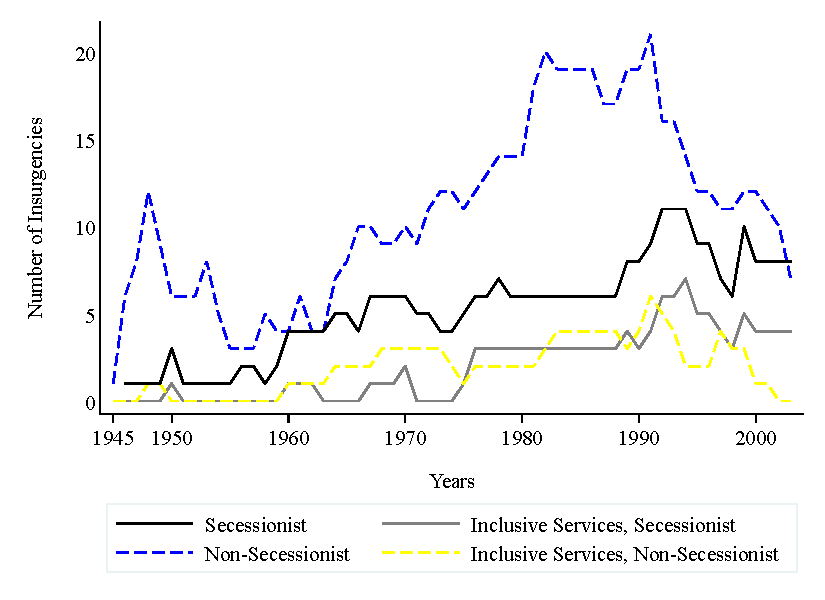
\includegraphics{pgedu.pdf}}
\end{center}
\begin{tablenotes}[para, flushleft]
\raggedright \footnotesize{\textit{Note:} The figure represents the number of insurgencies that provided inclusive education over time, conditional on territorial control. Dashed lines represent non-secessionist insurgencies and solid lines represent secessionist insurgencies. The proportion of secessionist insurgencies providing inclusive education to all secessionist insurgencies is much greater than the proportion of non-secessionist insurgencies providing inclusive education to all non-secessionist insurgencies. These data provide support for the hypothesis that secessionist insurgencies are more likely to provide inclusive services.} 
\end{tablenotes}
\end{figure}
\end{center}

\newpage
\clearpage
\begin{center}
\begin{figure}[h!]
\renewcommand\thefigure{A.\arabic{figure}}
\begin{center}
\caption{Insurgencies Providing Inclusive Health, by Strategic Goals}
\label{pghealth}
\scalebox{1}{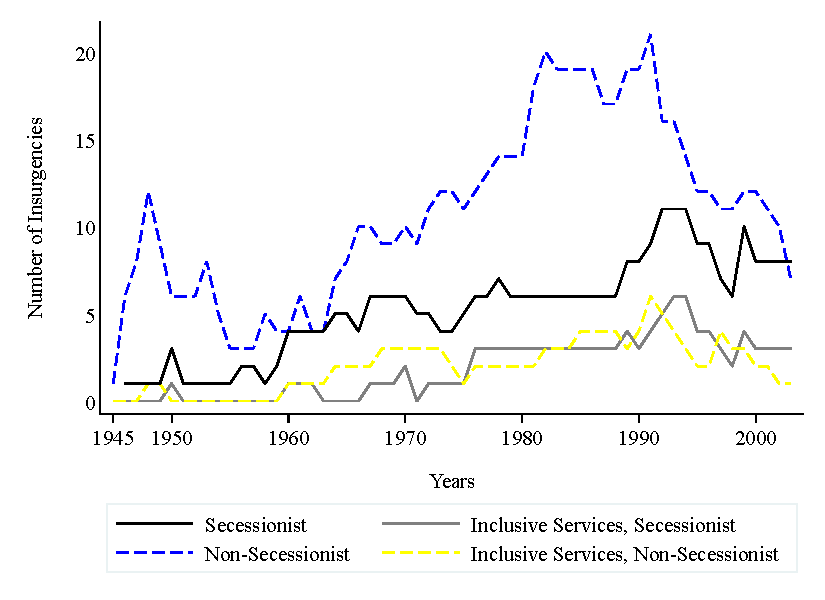
\includegraphics{pghealth.pdf}}
\end{center}
\begin{tablenotes}[para, flushleft]
\raggedright \footnotesize{\textit{Note:} \footnotesize The figure represents the number of insurgencies that provided inclusive health over time, conditional on territorial control. Dashed lines represent non-secessionist insurgencies and solid lines represent secessionist insurgencies. The proportion of secessionist insurgencies providing inclusive health to all secessionist insurgencies is much greater than the proportion of non-secessionist insurgencies providing inclusive health to all non-secessionist insurgencies. These data provide support for the hypothesis that secessionist insurgencies are more likely to provide inclusive services.} 
\end{tablenotes}
\end{figure}
\end{center}

\let\cleardoublepage\clearpage
\begin{table}[htbp]
\def\sym#1{\ifmmode^{#1}\else\(^{#1}\)\fi}
\renewcommand\thetable{A.\Roman{table}}
\caption{Summary Statistics, Panel Data}
\begin{tabular}{l*{1}{cccccc}}
\hline\hline
                    &\multicolumn{6}{c}{}                                                         \\
                    &        Mean&         Median&         Min&         Max&          SD&       Obs.\\
\hline
\textbf{All Insurgencies with Territory} \\
Secessionist        &        0.32&        0.00&        0.00&        1.00&        0.47&         943\\
Territorial Control &        1.00&        1.00&        1.00&        1.00&        0.00&         943\\
Communist           &        0.41&        0.00&        0.00&        1.00&        0.49&         943\\
Ethnic War          &        0.10&        0.00&        0.00&        1.00&        0.30&         943\\
Rebel Strength      &        0.87&        1.00&        0.00&        4.00&        0.76&         943\\
Duration            &       10.24&        7.00&        0.00&       54.00&       10.62&         943\\
Infant Mortality    &       84.38&       81.10&        5.20&      259.20&       45.62&         753\\
GDPpc               &        7.34&        7.28&        5.12&       10.05&        1.12&         632\\
Population (Logged) &       16.61&       16.68&       13.12&       20.76&        1.24&         701\\
Democracy           &        0.29&        0.00&        0.00&        1.00&        0.45&         876\\
Rugged Terrain      &        2.89&        3.50&        0.00&        4.31&        1.10&         942\\
Competition         &        3.16&        2.00&        1.00&       12.00&        2.22&         943\\
Population (Change) &       12.87&       13.05&        7.13&       16.66&        1.27&         642\\
\hline
\textbf{Secessionists (Territorial Control)} \\
Communist           &        0.27&        0.00&        0.00&        1.00&        0.45&         304\\
Ethnic War          &        0.00&        0.00&        0.00&        0.00&        0.00&         304\\
Rebel Strength      &        0.70&        1.00&        0.00&        3.00&        0.60&         304\\
Duration            &       11.43&        7.50&        0.00&       54.00&       12.33&         304\\
Infant Mortality    &       81.74&       80.70&        9.00&      178.00&       38.31&         256\\
GDPpc               &        7.15&        7.18&        5.49&        9.24&        0.87&         168\\
Population (Logged) &       17.22&       17.04&       13.15&       20.76&        1.48&         183\\
Democracy           &        0.22&        0.00&        0.00&        1.00&        0.41&         300\\
Ethnic War          &        0.99&        1.00&        0.00&        1.00&        0.11&         304\\
Rugged Terrain      &        3.12&        3.60&        0.00&        4.27&        1.08&         303\\
Competition         &        3.70&        2.50&        1.00&       12.00&        2.66&         304\\
Population (Change) &       13.25&       13.09&        7.52&       16.66&        1.59&         167\\
\hline
\textbf{Non-Secessionists (Territorial Control)} \\
Communist           &        0.47&        0.00&        0.00&        1.00&        0.50&         639\\
Ethnic War          &        0.15&        0.00&        0.00&        1.00&        0.36&         639\\
Rebel Strength      &        0.96&        1.00&        0.00&        4.00&        0.81&         639\\
Duration            &        9.67&        6.00&        0.00&       40.00&        9.66&         639\\
Infant Mortality    &       85.73&       82.70&        5.20&      259.20&       48.95&         497\\
GDPpc               &        7.41&        7.49&        5.12&       10.05&        1.19&         464\\
Population (Logged) &       16.40&       16.45&       13.12&       18.42&        1.06&         518\\
Democracy           &        0.32&        0.00&        0.00&        1.00&        0.47&         576\\
Ethnic War          &        0.15&        0.00&        0.00&        1.00&        0.36&         639\\
Rugged Terrain      &        2.78&        3.10&        0.34&        4.31&        1.09&         639\\
Competition         &        2.91&        2.00&        1.00&        7.00&        1.92&         639\\
Population (Change) &       12.74&       13.03&        7.13&       14.62&        1.11&         475\\
\hline\hline
\end{tabular}
\end{table}



\newpage
\begin{landscape}
\begin{table}[htbp]\centering
\begin{small}
\def\sym#1{\ifmmode^{#1}\else\(^{#1}\)\fi}
\renewcommand\thetable{A.\Roman{table}}
\newcounter{mym13}
\makeatletter
\def\myrow{}
\CT@everycr{\noalign{%
\global\let\CT@row@color\relax
\stepcounter{mym13}%
\ifnum\value{mym13}=2
  \gdef\myrow{\rowcolor{gray!50}}
\else\ifnum\value{mym13}=4
  \gdef\myrow{}
\fi\fi
}\myrow}
\caption{\textbf{Secessionism Predicts Inclusive Service Provision (Panel)}}
\label{table:conditionalp}
\begin{tabular}{l*{8}{c}}
\hline\hline
                    &\multicolumn{1}{c}{(1)}&\multicolumn{1}{c}{(2)}&\multicolumn{1}{c}{(3)}&\multicolumn{1}{c}{(4)}&\multicolumn{1}{c}{(5)}&\multicolumn{1}{c}{(6)}&\multicolumn{1}{c}{(7)}&\multicolumn{1}{c}{(8)}\\
Secessionist      &        0.26\sym{***}&        0.28\sym{**} &        0.27\sym{***}&        0.26\sym{**} &        0.18\sym{*}  &        0.21\sym{*}  &        0.49\sym{**} &        0.27\sym{**} \\
                    &      (0.09)         &      (0.12)         &      (0.10)         &      (0.11)         &      (0.10)         &      (0.11)         &      (0.18)         &      (0.11)         \\
Communist           &                     &        0.05         &                     &       -0.09         &       -0.01         &        0.04         &        0.64\sym{***}&       -0.07         \\
                    &                     &      (0.13)         &                     &      (0.16)         &      (0.15)         &      (0.12)         &      (0.13)         &      (0.17)         \\
Ethnic War          &                     &        0.07         &                     &       -0.11         &        0.09         &        0.15         &        0.57\sym{***}&       -0.18         \\
                    &                     &      (0.14)         &                     &      (0.14)         &      (0.12)         &      (0.13)         &      (0.16)         &      (0.16)         \\
Rebel Strength      &                     &       -0.01         &                     &       -0.08\sym{+}  &       -0.04         &       -0.05         &       -0.02         &       -0.09\sym{+}  \\
                    &                     &      (0.06)         &                     &      (0.05)         &      (0.05)         &      (0.04)         &      (0.07)         &      (0.06)         \\
Duration            &                     &        0.01         &                     &       -0.00         &       -0.01         &       -0.01\sym{**} &       -0.01         &       -0.00         \\
                    &                     &      (0.01)         &                     &      (0.00)         &      (0.00)         &      (0.00)         &      (0.01)         &      (0.00)         \\
Infant Mortality    &                     &                     &        0.00         &        0.00         &       -0.00         &        0.00         &       -0.00         &        0.00         \\
                    &                     &                     &      (0.00)         &      (0.00)         &      (0.00)         &      (0.00)         &      (0.00)         &      (0.00)         \\
GDPpc               &                     &                     &        0.07         &        0.05         &        0.12         &        0.18\sym{**} &       -0.29\sym{*}  &        0.04         \\
                    &                     &                     &      (0.08)         &      (0.08)         &      (0.09)         &      (0.07)         &      (0.15)         &      (0.08)         \\
Democracy           &                     &                     &       -0.18\sym{**} &       -0.20\sym{**} &       -0.01         &       -0.06         &        0.04         &       -0.20\sym{**} \\
                    &                     &                     &      (0.07)         &      (0.09)         &      (0.07)         &      (0.08)         &      (0.05)         &      (0.09)         \\
Population (Logged) &                     &                     &        0.08\sym{**} &        0.06\sym{+}  &        0.08\sym{*}  &        0.08\sym{*}  &        0.33\sym{*}  &                     \\
                    &                     &                     &      (0.04)         &      (0.04)         &      (0.04)         &      (0.04)         &      (0.20)         &                     \\
Rugged Terrain      &                     &                     &        0.01         &        0.03         &        0.06         &        0.09\sym{**} &                     &        0.03         \\
                    &                     &                     &      (0.04)         &      (0.04)         &      (0.05)         &      (0.04)         &                     &      (0.05)         \\
Population (Change) &                     &                     &                     &                     &                     &                     &                     &        0.03         \\
                    &                     &                     &                     &                     &                     &                     &                     &      (0.05)         \\
Competition         &                     &                     &                     &                     &                     &                     &                     &        0.02         \\
                    &                     &                     &                     &                     &                     &                     &                     &      (0.02)         \\
Constant            &        0.19\sym{***}&        0.06         &       -1.77\sym{*}  &       -1.14         &       -2.33\sym{*}  &       -3.12\sym{***}&       -3.33         &       -0.50         \\
                    &      (0.06)         &      (0.15)         &      (1.02)         &      (1.13)         &      (1.24)         &      (1.11)         &      (3.71)         &      (1.17)         \\
\\
Region FE             &         No                &           No              &               No          &      No                    &      Yes               & Yes                     &         No            &      No         \\
Decade FE            &         No                &           No              &               No          &      No                    &      No               & Yes                     &         No            &      No         \\
Country FE          &         No                &           No              &               No          &      No                    &      No               & No                     &         Yes            &      No         \\
\\                  
\hline
Observations        &         823         &         823         &         543         &         543         &         543         &         543         &         544         &         504         \\
\(R^{2}\)           &       0.072         &       0.139         &       0.204         &       0.225         &       0.305         &       0.370         &       0.653         &       0.210         \\
\hline\hline
\multicolumn{9}{l}{\footnotesize Standard errors in parentheses}\\
\multicolumn{9}{l}{\footnotesize Standard errors clustered by country in all models but Model 1.}\\
\multicolumn{9}{l}{\footnotesize \sym{+} \(p<0.15\), \sym{*} \(p<0.10\), \sym{**} \(p<0.05\), \sym{***} \(p<0.01\)}\\
\end{tabular}
\end{small}
\end{table}
\end{landscape}

\begin{landscape}
\begin{table}[htbp]\centering
\begin{footnotesize}
\def\sym#1{\ifmmode^{#1}\else\(^{#1}\)\fi}
\renewcommand\thetable{A.\Roman{table}}
\newcounter{mym14}
\makeatletter
\def\myrow{}
\CT@everycr{\noalign{%
\global\let\CT@row@color\relax
\stepcounter{mym14}%
\ifnum\value{mym14}=2
  \gdef\myrow{\rowcolor{gray!50}}
\else\ifnum\value{mym14}=8
  \gdef\myrow{}
\fi\fi
}\myrow}
\caption{\textbf{Secessionism Predicts Inclusive Services, Interaction (Panel)}}
\label{table:mainintp}
\begin{tabular}{l*{8}{c}}
\hline\hline
                    &\multicolumn{1}{c}{(1)}&\multicolumn{1}{c}{(2)}&\multicolumn{1}{c}{(3)}&\multicolumn{1}{c}{(4)}&\multicolumn{1}{c}{(5)}&\multicolumn{1}{c}{(6)}&\multicolumn{1}{c}{(7)}&\multicolumn{1}{c}{(8)}\\
\hline
Secessionist  $\times$ Territorial Control&        0.26\sym{***}&        0.26\sym{***}&        0.35\sym{***}&        0.38\sym{***}&        0.46\sym{***}&        0.46\sym{***}&        0.25\sym{**} &        0.32\sym{***}\\
                    &      (0.09)         &      (0.10)         &      (0.09)         &      (0.10)         &      (0.12)         &      (0.12)         &      (0.10)         &      (0.10)         \\
Secessionist      &        0.00         &       -0.00         &       -0.03         &       -0.07         &       -0.16\sym{*}  &       -0.15\sym{*}  &        0.12\sym{*}  &       -0.03         \\
                    &      (0.05)         &      (0.06)         &      (0.05)         &      (0.08)         &      (0.10)         &      (0.09)         &      (0.07)         &      (0.06)         \\
Territorial Control&        0.12\sym{**} &        0.08         &        0.06         &        0.07         &        0.06         &        0.07         &        0.01         &        0.08         \\
                    &      (0.06)         &      (0.06)         &      (0.05)         &      (0.06)         &      (0.06)         &      (0.05)         &      (0.06)         &      (0.06)         \\
Communist           &                     &       -0.02         &                     &       -0.10         &       -0.09         &       -0.08         &        0.11         &       -0.08         \\
                    &                     &      (0.07)         &                     &      (0.09)         &      (0.08)         &      (0.08)         &      (0.12)         &      (0.08)         \\
Ethnic War          &                     &       -0.00         &                     &       -0.08         &       -0.15\sym{+}  &       -0.14\sym{+}  &        0.09         &       -0.07         \\
                    &                     &      (0.08)         &                     &      (0.08)         &      (0.09)         &      (0.09)         &      (0.10)         &      (0.08)         \\
Rebel Strength      &                     &        0.01         &                     &       -0.02         &       -0.05\sym{*}  &       -0.05\sym{**} &       -0.00         &       -0.02         \\
                    &                     &      (0.03)         &                     &      (0.02)         &      (0.02)         &      (0.02)         &      (0.05)         &      (0.03)         \\
Duration            &                     &        0.01\sym{+}  &                     &        0.00         &        0.00         &        0.00         &       -0.00         &        0.00         \\
                    &                     &      (0.01)         &                     &      (0.00)         &      (0.00)         &      (0.00)         &      (0.00)         &      (0.00)         \\
Infant Mortality    &                     &                     &        0.00\sym{*}  &        0.00\sym{*}  &        0.00\sym{**} &        0.00\sym{**} &        0.00         &        0.00\sym{+}  \\
                    &                     &                     &      (0.00)         &      (0.00)         &      (0.00)         &      (0.00)         &      (0.00)         &      (0.00)         \\
GDPpc               &                     &                     &        0.06\sym{*}  &        0.06\sym{*}  &        0.06\sym{*}  &        0.07\sym{*}  &       -0.05         &        0.04         \\
                    &                     &                     &      (0.04)         &      (0.03)         &      (0.03)         &      (0.04)         &      (0.05)         &      (0.03)         \\
Democracy           &                     &                     &       -0.10\sym{+}  &       -0.11\sym{*}  &       -0.06         &       -0.07         &        0.00         &       -0.08\sym{*}  \\
                    &                     &                     &      (0.06)         &      (0.06)         &      (0.05)         &      (0.05)         &      (0.03)         &      (0.04)         \\
Population (Logged) &                     &                     &        0.03\sym{*}  &        0.03\sym{**} &        0.00         &        0.00         &        0.11         &                     \\
                    &                     &                     &      (0.01)         &      (0.01)         &      (0.02)         &      (0.02)         &      (0.08)         &                     \\
Rugged Terrain      &                     &                     &        0.02         &        0.04         &        0.06\sym{**} &        0.06\sym{**} &                     &        0.02         \\
                    &                     &                     &      (0.03)         &      (0.03)         &      (0.03)         &      (0.03)         &                     &      (0.03)         \\
Population (Change) &                     &                     &                     &                     &                     &                     &                     &        0.01         \\
                    &                     &                     &                     &                     &                     &                     &                     &      (0.01)         \\
Competition         &                     &                     &                     &                     &                     &                     &                     &        0.01         \\
                    &                     &                     &                     &                     &                     &                     &                     &      (0.01)         \\
Constant            &        0.07\sym{*}  &        0.02         &       -1.02\sym{***}&       -0.98\sym{**} &       -1.09\sym{***}&       -1.17\sym{***}&       -1.55         &       -0.54\sym{*}  \\
                    &      (0.04)         &      (0.06)         &      (0.36)         &      (0.39)         &      (0.34)         &      (0.37)         &      (1.17)         &      (0.31)         \\
\\
Region FE         &         No                &           No              &               No          &      No                    &      Yes               & Yes                     &         No            &      No         \\
Decade FE             &         No                &           No              &               No          &      No                    &      No               & Yes                     &         No            &      No         \\
Country FE                   &         No                &           No              &               No          &      No                    &      No               & No                     &         Yes            &      No         \\
\\   
\hline               
Observations        &        1897         &        1896         &        1384         &        1383         &        1383         &        1383         &        1387         &        1304         \\
\(R^{2}\)           &       0.116         &       0.160         &       0.191         &       0.210         &       0.267         &       0.283         &       0.562         &       0.185         \\
\hline\hline
\multicolumn{9}{l}{\footnotesize Standard errors in parentheses. Standard errors clustered by country in all models.}\\
\multicolumn{9}{l}{\footnotesize \sym{+} \(p<0.15\), \sym{*} \(p<0.10\), \sym{**} \(p<0.05\), \sym{***} \(p<0.01\)}\\
\end{tabular}
\end{footnotesize}
\end{table}
\end{landscape}


\begin{figure}[h]
\renewcommand\thefigure{A.\arabic{figure}}
\caption{\textbf{Predicted Effect of Secessionism on Inclusive Services (Panel)}}
\label{figure:mainpanel}
\centering
	\begin{subfigure}{0.45\textwidth}
    \centering
    \caption{Model 4, \autoref{table:conditionalp}} \label{figure:mainpanelcond}
    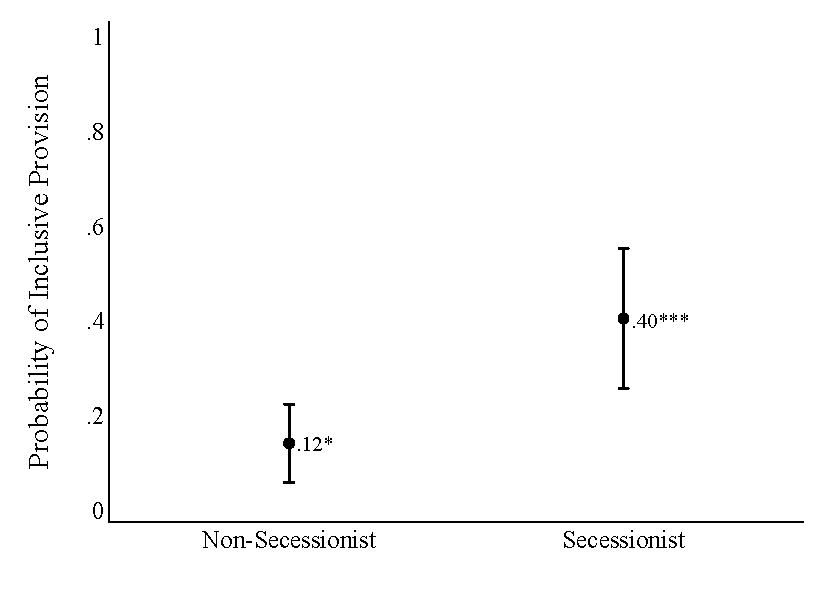
\includegraphics[width=\textwidth]{mainpanel.pdf}
    \end{subfigure}
% 
	\begin{subfigure}{0.45\textwidth}
    \centering
    \caption{Model 4, \autoref{table:mainintp}} \label{figure:mainpanelint}
    \includegraphics[width=\textwidth]{mainintpanel.pdf}
    \end{subfigure}
  \begin{tablenotes}[para, flushleft]
\raggedright \footnotesize{\textit{Note:} \autoref{figure:main} presents the predicted probability of \textit{Secessionist} rebel groups of providing inclusive services with all other variables set to their means. As is clear, secessionist rebel groups are between two to three times more likely to provide inclusive services than non-secessionist rebel groups. Moreover, the predicted probability between secessionist and non-secessionist groups is statistically significantly different, as confidence intervals fail to overlap. Black vertical lines represent 90\% confidence intervals.}
\end{tablenotes}
\end{figure}


\newpage
\begin{table}[htbp]\centering
\begin{small}
\def\sym#1{\ifmmode^{#1}\else\(^{#1}\)\fi}
\renewcommand\thetable{A.\Roman{table}}
\newcounter{mym15}
\makeatletter
\def\myrow{}
\CT@everycr{\noalign{%
\global\let\CT@row@color\relax
\stepcounter{mym15}%
\ifnum\value{mym15}=2
  \gdef\myrow{\rowcolor{gray!50}}
\else\ifnum\value{mym15}=4
  \gdef\myrow{}
\fi\fi
}\myrow}
\caption{\textbf{Additional Controls (Panel)}}
\label{table:addcontrolsp}
\begin{tabular}{l*{8}{c}}
\hline\hline
                    &\multicolumn{1}{c}{(1)}&\multicolumn{1}{c}{(2)}&\multicolumn{1}{c}{(3)}&\multicolumn{1}{c}{(4)}&\multicolumn{1}{c}{(5)}&\multicolumn{1}{c}{(6)}&\multicolumn{1}{c}{(7)}&\multicolumn{1}{c}{(8)}\\
\hline
Secessionist      &        0.26\sym{**} &        0.19\sym{+}  &        0.31\sym{***}&        0.23\sym{**} &        0.27\sym{**} &        0.24\sym{**} &        0.22\sym{*}  &        0.27\sym{**} \\
                    &      (0.11)         &      (0.12)         &      (0.11)         &      (0.11)         &      (0.11)         &      (0.12)         &      (0.13)         &      (0.11)         \\
Communist           &       -0.08         &       -0.10         &       -0.03         &       -0.08         &       -0.07         &       -0.03         &       -0.08         &       -0.10         \\
                    &      (0.17)         &      (0.17)         &      (0.15)         &      (0.16)         &      (0.16)         &      (0.14)         &      (0.13)         &      (0.19)         \\
Ethnic War          &       -0.20         &       -0.10         &       -0.20         &       -0.06         &       -0.11         &       -0.03         &       -0.07         &       -0.14         \\
                    &      (0.15)         &      (0.12)         &      (0.15)         &      (0.13)         &      (0.13)         &      (0.13)         &      (0.12)         &      (0.13)         \\
Rebel Strength      &       -0.11\sym{**} &       -0.05         &       -0.19\sym{**} &       -0.07         &       -0.06         &       -0.05         &       -0.05         &                     \\
                    &      (0.05)         &      (0.06)         &      (0.09)         &      (0.05)         &      (0.05)         &      (0.05)         &      (0.04)         &                     \\
Duration            &       -0.00         &       -0.00         &       -0.01\sym{+}  &       -0.00         &       -0.00         &        0.00         &        0.00         &       -0.00         \\
                    &      (0.00)         &      (0.00)         &      (0.00)         &      (0.00)         &      (0.00)         &      (0.00)         &      (0.00)         &      (0.00)         \\
Infant Mortality    &        0.00         &        0.00         &        0.00         &        0.00         &        0.00         &       -0.00         &       -0.00         &        0.00         \\
                    &      (0.00)         &      (0.00)         &      (0.00)         &      (0.00)         &      (0.00)         &      (0.00)         &      (0.00)         &      (0.00)         \\
GDPpc               &        0.05         &        0.07         &        0.05         &        0.06         &        0.05         &        0.01         &        0.01         &        0.05         \\
                    &      (0.08)         &      (0.08)         &      (0.08)         &      (0.07)         &      (0.08)         &      (0.07)         &      (0.08)         &      (0.08)         \\
Democracy           &       -0.19\sym{**} &       -0.25\sym{**} &       -0.09         &       -0.16\sym{*}  &       -0.22\sym{**} &       -0.17\sym{**} &       -0.16\sym{*}  &       -0.21\sym{**} \\
                    &      (0.09)         &      (0.10)         &      (0.10)         &      (0.08)         &      (0.08)         &      (0.07)         &      (0.08)         &      (0.09)         \\
Rugged Terrain      &        0.04         &        0.04         &       -0.01         &        0.05         &        0.02         &        0.04         &        0.03         &        0.04         \\
                    &      (0.05)         &      (0.05)         &      (0.04)         &      (0.04)         &      (0.05)         &      (0.04)         &      (0.04)         &      (0.05)         \\
Population (Change) &        0.04         &                     &                     &                     &                     &                     &                     &                     \\
                    &      (0.04)         &                     &                     &                     &                     &                     &                     &                     \\
Population (Logged) &                     &        0.10\sym{**} &        0.02         &        0.06         &        0.05         &        0.04         &        0.04         &        0.06         \\
                    &                     &      (0.04)         &      (0.05)         &      (0.04)         &      (0.04)         &      (0.04)         &      (0.03)         &      (0.04)         \\
Non-Military Aid    &                     &        0.15\sym{*}  &                     &                     &                     &                     &                     &                     \\
                    &                     &      (0.08)         &                     &                     &                     &                     &                     &                     \\
Rebel Group Size    &                     &                     &        0.13\sym{**} &                     &                     &                     &                     &                     \\
                    &                     &                     &      (0.05)         &                     &                     &                     &                     &                     \\
Battle Deaths       &                     &                     &                     &        0.02\sym{**} &                     &                     &                     &                     \\
                    &                     &                     &                     &      (0.01)         &                     &                     &                     &                     \\
Competition         &                     &                     &                     &                     &        0.02         &                     &                     &                     \\
                    &                     &                     &                     &                     &      (0.02)         &                     &                     &                     \\
Pre-Conflict Education&                     &                     &                     &                     &                     &        0.28\sym{+}  &                     &                     \\
                    &                     &                     &                     &                     &                     &      (0.18)         &                     &                     \\
Pre-Conflict Health &                     &                     &                     &                     &                     &                     &        0.24\sym{*}  &                     \\
                    &                     &                     &                     &                     &                     &                     &      (0.14)         &                     \\
Rebel Strength Categories         &                     &                     &                     &                     &                     &                     &                     &        Yes         \\
                    &                     &                     &                     &                     &                     &                     &                     &\\
Constant            &       -0.69         &       -1.93\sym{+}  &       -1.51         &       -1.33         &       -0.95         &       -0.56         &       -0.57         &       -1.16         \\
                    &      (1.11)         &      (1.15)         &      (1.10)         &      (1.09)         &      (1.20)         &      (1.01)         &      (1.06)         &      (1.04)         \\
\hline
Observations        &         504         &         422         &         510         &         526         &         543         &         500         &         500         &         543         \\
\(R^{2}\)           &       0.202         &       0.226         &       0.291         &       0.213         &       0.234         &       0.252         &       0.256         &       0.230         \\
\hline\hline
\multicolumn{9}{l}{\footnotesize Standard errors in parentheses}\\
\multicolumn{9}{l}{\footnotesize Standard errors clustered by country in all models.}\\
\multicolumn{9}{l}{\footnotesize \sym{+} \(p<0.15\), \sym{*} \(p<0.10\), \sym{**} \(p<0.05\), \sym{***} \(p<0.01\)}\\
\end{tabular}
\end{small}
\end{table}

\newpage
\begin{table}[htbp]\centering
\begin{small}
\def\sym#1{\ifmmode^{#1}\else\(^{#1}\)\fi}
\setcounter{table}{17}
\renewcommand\thetable{A.\Roman{table}}
\newcounter{mym16}
\makeatletter
\def\myrow{}
\CT@everycr{\noalign{%
\global\let\CT@row@color\relax
\stepcounter{mym16}%
\ifnum\value{mym16}=2
  \gdef\myrow{\rowcolor{gray!50}}
\else\ifnum\value{mym16}=4
  \gdef\myrow{}
\fi\fi
}\myrow}
\caption{\textbf{Additional Controls, Cont. (Panel)}}
\begin{tabular}{l*{4}{c}}
\hline\hline
                    &\multicolumn{1}{c}{(1)}&\multicolumn{1}{c}{(2)}&\multicolumn{1}{c}{(3)}&\multicolumn{1}{c}{(4)}\\
\hline
Secessionist     &        0.28\sym{+}  &        0.27\sym{*}  &        0.21\sym{+}  &        0.30\sym{*}  \\
                    &      (0.17)         &      (0.16)         &      (0.14)         &      (0.16)         \\
Communist           &        0.13         &        0.13         &        0.27         &        0.34\sym{**} \\
                    &      (0.22)         &      (0.22)         &      (0.20)         &      (0.15)         \\
Ethnic War          &       -0.38\sym{+}  &       -0.49\sym{**} &       -0.01         &        0.11         \\
                    &      (0.25)         &      (0.23)         &      (0.32)         &      (0.29)         \\
Duration            &       -0.00         &       -0.00         &       -0.01         &       -0.01\sym{***}\\
                    &      (0.01)         &      (0.01)         &      (0.01)         &      (0.00)         \\
Infant Mortality    &       -0.00         &       -0.00         &       -0.00\sym{**} &       -0.00         \\
                    &      (0.00)         &      (0.00)         &      (0.00)         &      (0.00)         \\
GDPpc               &       -0.08         &       -0.07         &       -0.03         &        0.07         \\
                    &      (0.08)         &      (0.10)         &      (0.08)         &      (0.07)         \\
Democracy           &       -0.17\sym{+}  &       -0.20\sym{+}  &       -0.06         &       -0.05         \\
                    &      (0.11)         &      (0.13)         &      (0.09)         &      (0.10)         \\
Population (Logged) &       -0.02         &                     &        0.01         &       -0.00         \\
                    &      (0.04)         &                     &      (0.04)         &      (0.04)         \\
Rugged Terrain      &        0.01         &        0.00         &        0.02         &        0.05         \\
                    &      (0.06)         &      (0.06)         &      (0.07)         &      (0.05)         \\
Population (Change) &                     &        0.01         &                     &                     \\
                    &                     &      (0.04)         &                     &                     \\
Non-Military Aid    &        0.02         &        0.05         &       -0.00         &       -0.05         \\
                    &      (0.07)         &      (0.08)         &      (0.09)         &      (0.08)         \\
Rebel Group Size    &        0.18\sym{**} &        0.18\sym{**} &        0.19\sym{**} &        0.21\sym{***}\\
                    &      (0.08)         &      (0.08)         &      (0.07)         &      (0.06)         \\
Competition         &       -0.01         &       -0.02         &        0.00         &        0.00         \\
                    &      (0.02)         &      (0.02)         &      (0.02)         &      (0.02)         \\
Battle Deaths       &       -0.01         &       -0.01         &        0.00         &       -0.00         \\
                    &      (0.01)         &      (0.01)         &      (0.01)         &      (0.01)         \\
Pre-Conflict Education&        0.49\sym{**} &        0.40\sym{*}  &        0.80\sym{***}&        0.68\sym{***}\\
                    &      (0.21)         &      (0.20)         &      (0.20)         &      (0.20)         \\
Pre-Conflict Health &       -0.00         &        0.05         &       -0.16         &       -0.20         \\
                    &      (0.17)         &      (0.16)         &      (0.17)         &      (0.14)         \\
Rebel Strength Categories      &         Yes  &         Yes &       Yes &       Yes  \\
                    &          &              &               &               \\
Constant            &       -0.59         &       -0.97         &       -0.99         &       -2.40\sym{***}\\
                    &      (1.17)         &      (1.33)         &      (0.97)         &      (0.83)         \\
\\
Region Fixed Effects               &      No               &         No            &         Yes            &      Yes     \\
Decade Fixed Effects               &      No               &         No            &         No            &      Yes     \\                    
\hline
Observations        &         386         &         356         &         386         &         386         \\
\(R^{2}\)           &       0.436         &       0.418         &       0.526         &       0.578         \\
\hline\hline
\multicolumn{5}{l}{\footnotesize Standard errors in parentheses.}\\
\multicolumn{5}{l}{\footnotesize Standard errors clustered by country in all models.}\\
\multicolumn{5}{l}{\footnotesize \sym{+} \(p<0.15\), \sym{*} \(p<0.10\), \sym{**} \(p<0.05\), \sym{***} \(p<0.01\)}\\
\end{tabular}
\end{small}
\end{table}


\newpage
\begin{table}[htbp]\centering
\begin{small}
\def\sym#1{\ifmmode^{#1}\else\(^{#1}\)\fi}
\renewcommand\thetable{A.\Roman{table}}
\newcounter{mym17}
\makeatletter
\def\myrow{}
\CT@everycr{\noalign{%
\global\let\CT@row@color\relax
\stepcounter{mym17}%
\ifnum\value{mym17}=2
  \gdef\myrow{\rowcolor{gray!50}}
\else\ifnum\value{mym17}=4
  \gdef\myrow{}
\fi\fi
}\myrow}
\caption{\textbf{Excluding Outliers (Panel)}}
\begin{tabular}{l*{1}{c}}
\hline\hline
                    &\multicolumn{1}{c}{(1)}\\
\hline
Secessionist      &        0.31\sym{***}\\
                    &      (0.09)         \\
Communist           &        0.03         \\
                    &      (0.15)         \\
Ethnic War          &       -0.11         \\
                    &      (0.15)         \\
Rebel Strength      &       -0.03         \\
                    &      (0.04)         \\
Duration            &       -0.00         \\
                    &      (0.00)         \\
Infant Mortality    &        0.00         \\
                    &      (0.00)         \\
GDPpc               &        0.09         \\
                    &      (0.07)         \\
Democracy           &       -0.22\sym{**} \\
                    &      (0.11)         \\
Population (Logged) &        0.10\sym{**} \\
                    &      (0.05)         \\
Rugged Terrain      &        0.02         \\
                    &      (0.04)         \\
Constant            &       -2.39\sym{*}  \\
                    &      (1.27)         \\
\hline
Observations        &         509         \\
\(R^{2}\)           &       0.372         \\
\hline\hline
\multicolumn{2}{l}{\footnotesize Standard errors in parentheses.}\\
\multicolumn{2}{l}{\footnotesize Standard errors clustered by country in all models.}\\
\multicolumn{2}{l}{\footnotesize \sym{+} \(p<0.15\), \sym{*} \(p<0.10\), \sym{**} \(p<0.05\), \sym{***} \(p<0.01\)}\\
\end{tabular}
\end{small}
\end{table}

\newpage
\begin{table}[htbp]\centering
\begin{small}
\def\sym#1{\ifmmode^{#1}\else\(^{#1}\)\fi}
\renewcommand\thetable{A.\Roman{table}}
\newcounter{mym18}
\makeatletter
\def\myrow{}
\CT@everycr{\noalign{%
\global\let\CT@row@color\relax
\stepcounter{mym18}%
\ifnum\value{mym18}=2
  \gdef\myrow{\rowcolor{gray!50}}
\else\ifnum\value{mym18}=4
  \gdef\myrow{}
\fi\fi
}\myrow}
\caption{\textbf{Jackknifing (Panel)}}
\begin{tabular}{l*{1}{c}}
\hline\hline
                    &\multicolumn{1}{c}{(1)}\\
\hline
Secessionist      &        0.26\sym{***}\\
                    &      (0.04)         \\
Communist           &       -0.09\sym{*}  \\
                    &      (0.05)         \\
Ethnic War          &       -0.11\sym{+}  \\
                    &      (0.08)         \\
Rebel Strength      &       -0.08\sym{***}\\
                    &      (0.02)         \\
Duration            &       -0.00         \\
                    &      (0.00)         \\
Infant Mortality    &        0.00         \\
                    &      (0.00)         \\
GDPpc               &        0.05\sym{*}  \\
                    &      (0.03)         \\
Democracy           &       -0.20\sym{***}\\
                    &      (0.04)         \\
Population (Logged) &        0.06\sym{***}\\
                    &      (0.02)         \\
Rugged Terrain      &        0.03\sym{**} \\
                    &      (0.02)         \\
Constant            &       -1.14\sym{**} \\
                    &      (0.52)         \\
\hline
Observations        &         543         \\
\(R^{2}\)           &       0.225         \\
\hline\hline
\multicolumn{2}{l}{\footnotesize Standard errors in parentheses.}\\
\multicolumn{2}{l}{\footnotesize \sym{+} \(p<0.15\), \sym{*} \(p<0.10\), \sym{**} \(p<0.05\), \sym{***} \(p<0.01\)}\\
\end{tabular}
\end{small}
\end{table}

\newpage
\begin{table}[htbp]\centering
\begin{small}
\def\sym#1{\ifmmode^{#1}\else\(^{#1}\)\fi}
\renewcommand\thetable{A.\Roman{table}}
\newcounter{mym19}
\makeatletter
\def\myrow{}
\CT@everycr{\noalign{%
\global\let\CT@row@color\relax
\stepcounter{mym19}%
\ifnum\value{mym19}=2
  \gdef\myrow{\rowcolor{gray!50}}
\else\ifnum\value{mym19}=4
  \gdef\myrow{}
\fi\fi
}\myrow}
\caption{\textbf{Original Dataset (Panel)}}
\begin{tabular}{l*{1}{c}}
\hline\hline
                    &\multicolumn{1}{c}{(1)}\\
\hline
Secessionist      &        0.25\sym{**} \\
                    &      (0.11)         \\
Communist           &       -0.11         \\
                    &      (0.17)         \\
Ethnic War          &       -0.21         \\
                    &      (0.17)         \\
Rebel Strength      &       -0.12\sym{*}  \\
                    &      (0.07)         \\
Duration            &       -0.00         \\
                    &      (0.00)         \\
Infant Mortality    &        0.00         \\
                    &      (0.00)         \\
GDPpc               &        0.08         \\
                    &      (0.08)         \\
Democracy           &       -0.18\sym{*}  \\
                    &      (0.10)         \\
Population (Logged) &        0.04         \\
                    &      (0.04)         \\
Rugged Terrain      &        0.02         \\
                    &      (0.04)         \\
Constant            &       -1.00         \\
                    &      (1.18)         \\
\hline
Observations        &         543         \\
\(R^{2}\)           &       0.207         \\
\hline\hline
\multicolumn{2}{l}{\footnotesize Standard errors in parentheses.}\\
\multicolumn{2}{l}{\footnotesize Standard errors clustered by country in all models.}\\
\multicolumn{2}{l}{\footnotesize \sym{+} \(p<0.15\), \sym{*} \(p<0.10\), \sym{**} \(p<0.05\), \sym{***} \(p<0.01\)}\\
\end{tabular}
\end{small}
\end{table}

\newpage
\begin{table}[htbp]\centering
\begin{small}
\def\sym#1{\ifmmode^{#1}\else\(^{#1}\)\fi}
\renewcommand\thetable{A.\Roman{table}}
\newcounter{mym20}
\makeatletter
\def\myrow{}
\CT@everycr{\noalign{%
\global\let\CT@row@color\relax
\stepcounter{mym20}%
\ifnum\value{mym20}=4
  \gdef\myrow{\rowcolor{gray!50}}
\else\ifnum\value{mym20}=6
  \gdef\myrow{}
\fi\fi
}\myrow}
\caption{\textbf{Correcting for Information Bias (Panel)}}
\label{table:infop}
\begin{tabular}{l*{3}{c}}
\hline\hline
                    &\multicolumn{1}{c}{(1)}&\multicolumn{1}{c}{(2)}&\multicolumn{1}{c}{(3)}\\
                    &\multicolumn{1}{c}{Large}&\multicolumn{1}{c}{Post-1970}&\multicolumn{1}{c}{No Missingness,}\\
  &\multicolumn{1}{c}{Insurgencies}&\multicolumn{1}{c}{Insurgencies}&\multicolumn{1}{c}{No Services}\\
\hline
Secessionist      &        0.56\sym{***}&        0.35\sym{**} &        0.27\sym{**} \\
                    &      (0.14)         &      (0.13)         &      (0.11)         \\
Rebel Strength      &       -0.04         &       -0.18\sym{**} &       -0.07         \\
                    &      (0.07)         &      (0.07)         &      (0.05)         \\
Communist           &        0.15         &       -0.27\sym{**} &       -0.09         \\
                    &      (0.25)         &      (0.12)         &      (0.16)         \\
Ethnic War          &        0.00         &       -0.25\sym{+}  &       -0.11         \\
                    &      (0.18)         &      (0.16)         &      (0.14)         \\
Duration            &       -0.00         &        0.01\sym{+}  &       -0.00         \\
                    &      (0.00)         &      (0.01)         &      (0.00)         \\
Infant Mortality    &       -0.00\sym{+}  &        0.00\sym{*}  &        0.00         \\
                    &      (0.00)         &      (0.00)         &      (0.00)         \\
GDPpc               &       -0.08         &        0.11\sym{+}  &        0.05         \\
                    &      (0.09)         &      (0.07)         &      (0.08)         \\
Population (Logged) &       -0.03         &        0.01         &        0.06\sym{+}  \\
                    &      (0.08)         &      (0.04)         &      (0.04)         \\
Democracy           &       -0.22\sym{*}  &       -0.17\sym{**} &       -0.19\sym{**} \\
                    &      (0.11)         &      (0.08)         &      (0.08)         \\
Rugged Terrain      &       -0.08         &        0.11\sym{**} &        0.03         \\
                    &      (0.08)         &      (0.04)         &      (0.04)         \\
Constant            &        1.81         &       -1.04         &       -1.17         \\
                    &      (1.82)         &      (1.10)         &      (1.13)         \\
\hline
Observations        &         319         &         404         &         556         \\
\(R^{2}\)           &       0.353         &       0.338         &       0.224         \\
\hline\hline
\multicolumn{4}{l}{\footnotesize Standard errors in parentheses}\\
\multicolumn{4}{l}{\footnotesize Standard errors clustered by country in all models.}\\
\multicolumn{4}{l}{\footnotesize \sym{+} \(p<0.15\), \sym{*} \(p<0.10\), \sym{**} \(p<0.05\), \sym{***} \(p<0.01\)}\\
\end{tabular}
\end{small}
\end{table}

\newpage
\begin{table}[htbp]\centering
\begin{small}
\def\sym#1{\ifmmode^{#1}\else\(^{#1}\)\fi}
\renewcommand\thetable{A.\Roman{table}}
\newcounter{mym21}
\makeatletter
\def\myrow{}
\CT@everycr{\noalign{%
\global\let\CT@row@color\relax
\stepcounter{mym21}%
\ifnum\value{mym21}=2
  \gdef\myrow{\rowcolor{gray!50}}
\else\ifnum\value{mym21}=8
  \gdef\myrow{}
\fi\fi
}\myrow}
\caption{\textbf{Alternative Secessionist Specification (Panel)}}
\begin{tabular}{l*{3}{c}}
\hline\hline
                    &\multicolumn{1}{c}{(1)}&\multicolumn{1}{c}{(2)}&\multicolumn{1}{c}{(3)}\\
\hline
Secessionist (Broadly Defined)&        0.26\sym{**} &                     &                     \\
                    &      (0.11)         &                     &                     \\
Secessionist (Broadly Defined) &                     &        0.32\sym{***}&                     \\
                    &                     &      (0.10)         &                     \\
Secessionist (Broadly Defined)&                     &                     &        0.31\sym{***}\\
                    &                     &                     &      (0.10)         \\
Communist           &       -0.09         &       -0.05         &       -0.05         \\
                    &      (0.16)         &      (0.16)         &      (0.16)         \\
Ethnic War          &       -0.11         &       -0.04         &       -0.31\sym{**} \\
                    &      (0.14)         &      (0.14)         &      (0.13)         \\
Rebel Strength      &       -0.08\sym{+}  &       -0.05         &       -0.05         \\
                    &      (0.05)         &      (0.05)         &      (0.05)         \\
Duration            &       -0.00         &       -0.00         &       -0.00         \\
                    &      (0.00)         &      (0.00)         &      (0.00)         \\
Infant Mortality    &        0.00         &        0.00         &        0.00         \\
                    &      (0.00)         &      (0.00)         &      (0.00)         \\
GDPpc               &        0.05         &        0.04         &        0.03         \\
                    &      (0.08)         &      (0.07)         &      (0.07)         \\
Democracy           &       -0.20\sym{**} &       -0.20\sym{**} &       -0.19\sym{**} \\
                    &      (0.09)         &      (0.08)         &      (0.08)         \\
Population (Logged) &        0.06\sym{+}  &        0.06\sym{+}  &        0.06\sym{+}  \\
                    &      (0.04)         &      (0.04)         &      (0.04)         \\
Rugged Terrain      &        0.03         &        0.04         &        0.04         \\
                    &      (0.04)         &      (0.05)         &      (0.04)         \\
Constant            &       -1.14         &       -1.21         &       -1.14         \\
                    &      (1.13)         &      (1.13)         &      (1.14)         \\
\hline
Observations        &         543         &         543         &         543         \\
\(R^{2}\)           &       0.225         &       0.265         &       0.257         \\
\hline\hline
\multicolumn{4}{l}{\footnotesize Standard errors in parentheses}\\
\multicolumn{4}{l}{\footnotesize Standard errors clustered by country in all models.}\\
\multicolumn{4}{l}{\footnotesize \sym{+} \(p<0.15\), \sym{*} \(p<0.10\), \sym{**} \(p<0.05\), \sym{***} \(p<0.01\)}\\
\end{tabular}
\end{small}
\end{table}

\newpage
\begin{table}[htbp]\centering
\begin{small}
\def\sym#1{\ifmmode^{#1}\else\(^{#1}\)\fi}
\renewcommand\thetable{A.\Roman{table}}
\newcounter{mym22}
\makeatletter
\def\myrow{}
\CT@everycr{\noalign{%
\global\let\CT@row@color\relax
\stepcounter{mym22}%
\ifnum\value{mym22}=3
  \gdef\myrow{\rowcolor{gray!50}}
\else\ifnum\value{mym22}=5
  \gdef\myrow{}
\fi\fi
}\myrow}
\caption{\textbf{Alternative Inclusive Services Specification (Panel)}}
\label{table:altpgp}
\begin{tabular}{l*{3}{c}}
\hline\hline
                    &\multicolumn{1}{c}{(1)}&\multicolumn{1}{c}{(2)}&\multicolumn{1}{c}{(3)}\\
                                        &\multicolumn{1}{c}{Any Inclusive Services}&\multicolumn{1}{c}{Alternative Coding}&\multicolumn{1}{c}{Ordinal Ranking}\\
\hline
Secessionist      &        0.39\sym{**} &        0.26\sym{**} &        0.41\sym{***}\\
                    &      (0.16)         &      (0.12)         &      (0.14)         \\
Communist           &        0.01         &       -0.08         &        0.07         \\
                    &      (0.19)         &      (0.17)         &      (0.20)         \\
Ethnic War          &        0.51\sym{**} &       -0.23         &       -0.05         \\
                    &      (0.20)         &      (0.16)         &      (0.22)         \\
Rebel Strength      &       -0.14\sym{*}  &       -0.13\sym{*}  &       -0.17\sym{**} \\
                    &      (0.07)         &      (0.06)         &      (0.08)         \\
Duration            &       -0.01\sym{*}  &       -0.00         &        0.00         \\
                    &      (0.00)         &      (0.00)         &      (0.00)         \\
Infant Mortality    &       -0.00         &        0.00         &        0.00         \\
                    &      (0.00)         &      (0.00)         &      (0.00)         \\
GDPpc               &        0.03         &        0.12         &        0.12         \\
                    &      (0.09)         &      (0.09)         &      (0.11)         \\
Democracy           &       -0.22\sym{*}  &       -0.20\sym{*}  &       -0.13         \\
                    &      (0.12)         &      (0.10)         &      (0.11)         \\
Population (Logged) &        0.05         &        0.03         &        0.05         \\
                    &      (0.06)         &      (0.04)         &      (0.07)         \\
Rugged Terrain      &       -0.02         &        0.01         &        0.02         \\
                    &      (0.06)         &      (0.05)         &      (0.05)         \\
Constant            &       -0.41         &       -1.17         &       -0.87         \\
                    &      (1.43)         &      (1.18)         &      (1.86)         \\
\hline
Observations        &         561         &         546         &         561         \\
\(R^{2}\)           &       0.404         &       0.206         &       0.225         \\
\hline\hline
\multicolumn{4}{l}{\footnotesize Standard errors in parentheses}\\
\multicolumn{4}{l}{\footnotesize Standard errors clustered by country in all models.}\\
\multicolumn{4}{l}{\footnotesize \sym{+} \(p<0.15\), \sym{*} \(p<0.10\), \sym{**} \(p<0.05\), \sym{***} \(p<0.01\)}\\
\end{tabular}
\end{small}
\end{table}

\newpage
\begin{table}[htbp]\centering
\begin{small}
\def\sym#1{\ifmmode^{#1}\else\(^{#1}\)\fi}
\renewcommand\thetable{A.\Roman{table}}
\newcounter{mym23}
\makeatletter
\def\myrow{}
\CT@everycr{\noalign{%
\global\let\CT@row@color\relax
\stepcounter{mym23}%
\ifnum\value{mym23}=3
  \gdef\myrow{\rowcolor{gray!50}}
\else\ifnum\value{mym23}=5
  \gdef\myrow{}
\fi\fi
}\myrow}
\caption{\textbf{Alternative Estimator (Panel)}}
\begin{tabular}{l*{2}{c}}
\hline\hline
                    &\multicolumn{1}{c}{(1)}&\multicolumn{1}{c}{(2)}\\
                    &\multicolumn{1}{c}{Logit}&\multicolumn{1}{c}{Ordered Logit}\\
\hline
Secessionist      &        1.54\sym{**} &        1.90\sym{**} \\
                    &      (0.71)         &      (0.77)         \\
Communist           &       -0.63         &        0.38         \\
                    &      (1.18)         &      (0.93)         \\
Ethnic War          &       -1.21         &       -0.18         \\
                    &      (1.01)         &      (1.06)         \\
Rebel Strength      &       -0.98\sym{*}  &       -0.69\sym{**} \\
                    &      (0.52)         &      (0.34)         \\
Duration            &       -0.01         &        0.02         \\
                    &      (0.03)         &      (0.02)         \\
Infant Mortality    &       -0.00         &        0.01         \\
                    &      (0.01)         &      (0.01)         \\
GDPpc               &        0.27         &        0.62         \\
                    &      (0.60)         &      (0.51)         \\
Democracy           &       -1.82\sym{***}&       -0.62         \\
                    &      (0.68)         &      (0.52)         \\
Population (Logged) &        0.32         &        0.30         \\
                    &      (0.32)         &      (0.31)         \\
Rugged Terrain      &        0.31         &        0.06         \\
                    &      (0.37)         &      (0.23)         \\
Constant            &       -8.18         &                     \\
                    &      (7.60)         &                     \\
\hline
cut1                &                     &                     \\
Constant            &                     &        8.42         \\
                    &                     &      (8.21)         \\
\hline
cut2                &                     &                     \\
Constant            &                     &       12.60\sym{+}  \\
                    &                     &      (8.59)         \\
\hline
Observations        &         543         &         561         \\
\(R^{2}\)           &            0.227          &         0.159            \\
\hline\hline
\multicolumn{3}{l}{\footnotesize Standard errors in parentheses.}\\
\multicolumn{3}{l}{\footnotesize Standard errors clustered by country in all models.}\\
\multicolumn{3}{l}{\footnotesize \sym{+} \(p<0.15\), \sym{*} \(p<0.10\), \sym{**} \(p<0.05\), \sym{***} \(p<0.01\)}\\
\end{tabular}
\end{small}
\end{table}



\newpage
\begin{table}[htbp]\centering
\begin{small}
\def\sym#1{\ifmmode^{#1}\else\(^{#1}\)\fi}
\renewcommand\thetable{A.\Roman{table}}
\newcounter{mym124}
\makeatletter
\def\myrow{}
\CT@everycr{\noalign{%
\global\let\CT@row@color\relax
\stepcounter{mym124}%
\ifnum\value{mym124}=3
  \gdef\myrow{\rowcolor{gray!50}}
\else\ifnum\value{mym124}=5
  \gdef\myrow{}
\fi\fi
}\myrow}
\caption{\textbf{Multiple Imputation (Panel)}}
\begin{tabular}{l*{1}{c}}
\hline\hline
                    &\multicolumn{1}{c}{(1)}\\
                    &\multicolumn{1}{c}{Public Goods}\\
\hline
Secessionist        &        0.24\sym{**} \\
                    &      (0.11)         \\
Communist           &        0.07         \\
                    &      (0.13)         \\
Ethnic War          &        0.00         \\
                    &      (0.16)         \\
Rebel Strength      &       -0.04         \\
                    &      (0.05)         \\
Duration            &        0.01\sym{+}  \\
                    &      (0.01)         \\
Infant Mortality    &        0.00         \\
                    &      (0.00)         \\
GDPpc               &        0.03         \\
                    &      (0.05)         \\
Democracy           &       -0.26\sym{***}\\
                    &      (0.08)         \\
Population (Logged) &        0.01         \\
                    &      (0.03)         \\
Rugged Terrain      &        0.02         \\
                    &      (0.04)         \\
\hline
Observations        &         822         \\
\hline\hline
\hline\hline
\multicolumn{2}{l}{\footnotesize Standard errors in parentheses.}\\
\multicolumn{2}{l}{\footnotesize Standard errors clustered by country in all models.}\\
\multicolumn{2}{l}{\footnotesize \sym{+} \(p<0.15\), \sym{*} \(p<0.10\), \sym{**} \(p<0.05\), \sym{***} \(p<0.01\)}\\
\end{tabular}
\end{small}
\end{table}


\begin{figure}[h]
\renewcommand\thefigure{A.\arabic{figure}}
\caption{\textbf{ROC Curves of Predicted Accuracy}}
\label{figure:roccurvep}
\centering
	\begin{subfigure}{0.45\textwidth}
    \centering
    \caption{Model 4, \autoref{table:conditionalp}} \label{figure:roccurve1p}
    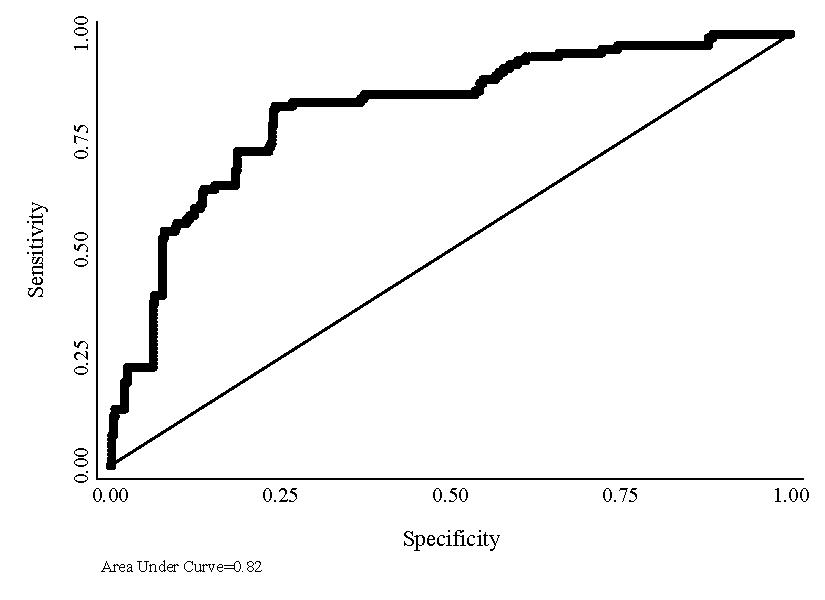
\includegraphics[width=\textwidth]{roccurve1p.pdf}
    \end{subfigure}
% 
	\begin{subfigure}{0.45\textwidth}
    \centering
    \caption{Model 4, \autoref{table:mainintp}} \label{figure:roccurve2p}
    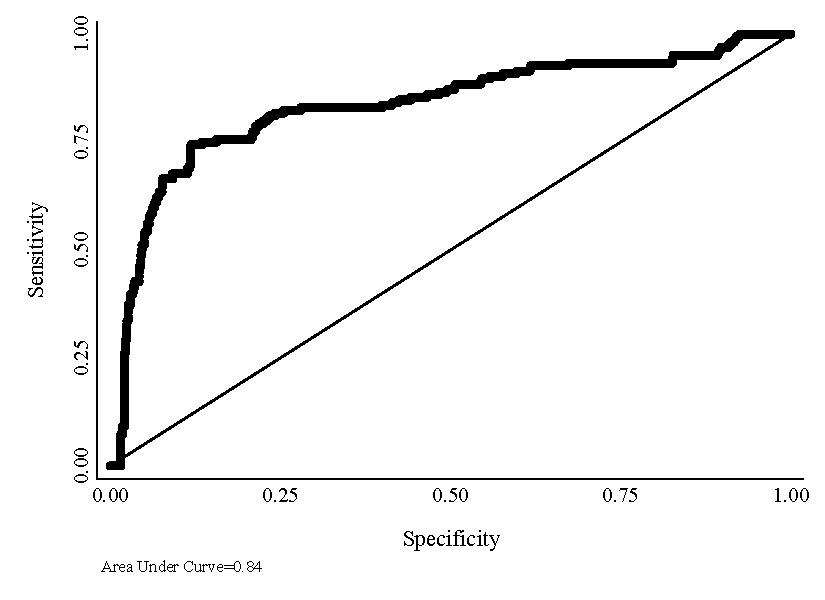
\includegraphics[width=\textwidth]{roccurve2p.pdf}
    \end{subfigure}
  \begin{tablenotes}[para, flushleft]
\raggedright \footnotesize{\textit{Note:} The figure demonstrates the predictive power of Model 4 in  \autoref{table:conditionalp}. The AUC for Model 4, \autoref{table:conditionalp} is 0.82 and the AUC for Model 4, \autoref{table:mainintp} is 0.84 meaning that the model is highly capable of correctly predicting insurgencies likely to provide inclusive services.}
\end{tablenotes}
\end{figure}



\newpage
\begin{table}[htbp]\centering
\begin{small}
\def\sym#1{\ifmmode^{#1}\else\(^{#1}\)\fi}
\renewcommand\thetable{A.\Roman{table}}
\newcounter{mym24}
\makeatletter
\def\myrow{}
\CT@everycr{\noalign{%
\global\let\CT@row@color\relax
\stepcounter{mym24}%
\ifnum\value{mym24}=2
  \gdef\myrow{\rowcolor{gray!50}}
\else\ifnum\value{mym24}=4
  \gdef\myrow{}
\fi\fi
}\myrow}
\caption{\textbf{Bootstrapping (Panel)}}
\begin{tabular}{l*{1}{c}}
\hline\hline
                    &\multicolumn{1}{c}{(1)}\\
\hline
Secessionist      &        0.26\sym{***}\\
                    &      (0.07)         \\
Communist           &       -0.09         \\
                    &      (0.07)         \\
Ethnic War          &       -0.11         \\
                    &      (0.12)         \\
Rebel Strength      &       -0.08\sym{**} \\
                    &      (0.03)         \\
Duration            &       -0.00         \\
                    &      (0.00)         \\
Infant Mortality    &        0.00         \\
                    &      (0.00)         \\
GDPpc               &        0.05         \\
                    &      (0.05)         \\
Democracy           &       -0.20\sym{***}\\
                    &      (0.06)         \\
Population (Logged) &        0.06\sym{**} \\
                    &      (0.03)         \\
Rugged Terrain      &        0.03         \\
                    &      (0.02)         \\
Constant            &       -1.14\sym{+}  \\
                    &      (0.78)         \\
\hline
Observations        &         543         \\
\(R^{2}\)           &       0.225         \\
\hline\hline
\multicolumn{2}{l}{\footnotesize Standard errors in parentheses}\\
\multicolumn{2}{l}{\footnotesize \sym{+} \(p<0.15\), \sym{*} \(p<0.10\), \sym{**} \(p<0.05\), \sym{***} \(p<0.01\)}\\
\end{tabular}
\end{small}
\end{table}

\newpage
\begin{figure}[h]
\renewcommand\thefigure{A.\arabic{figure}}
\caption{\textbf{Comparison of Cross-Sectional and Panel Secessionist Coefficient Estimates}}
\label{figure:coefcomp1}
\centering
	\begin{subfigure}{0.45\textwidth}
    \centering
    \caption{\autoref{table:conditional}} \label{figure:coefmaincomp}
    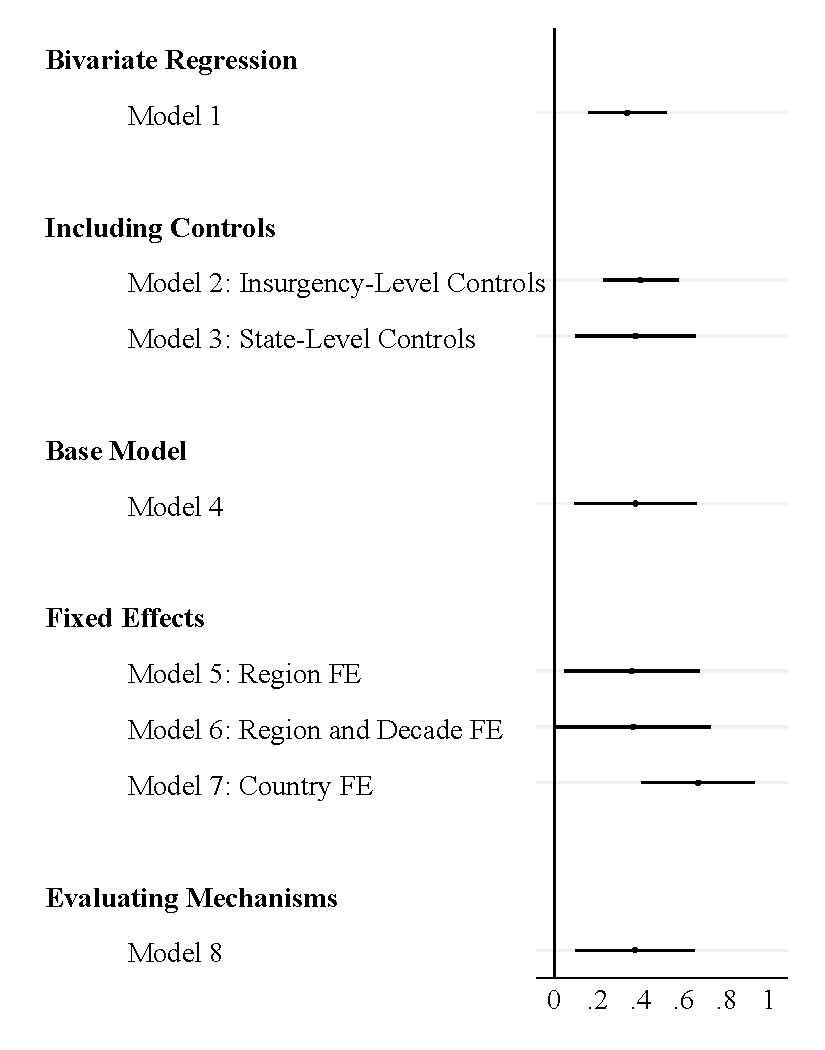
\includegraphics[width=\textwidth]{coefmain.pdf}
    \end{subfigure}
% 
	\begin{subfigure}{0.45\textwidth}
    \centering
    \caption{\autoref{table:conditionalp}} \label{figure:coefpanel}
    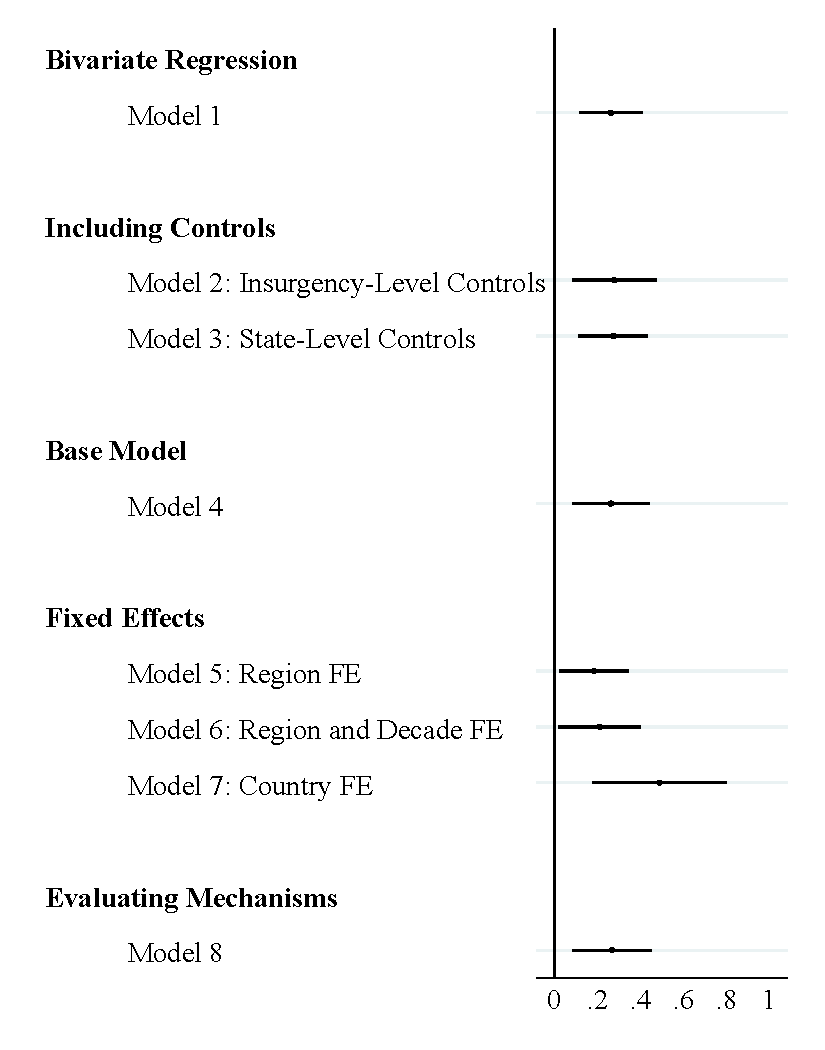
\includegraphics[width=\textwidth]{coefpanel.pdf}
    \end{subfigure}
  \begin{tablenotes}[para, flushleft]
\raggedright \footnotesize{\textit{Note:} \autoref{figure:coefcomp1} presents the coefficient estimates for the variable \textit{Secessionist} in \autoref{table:conditional} and \autoref{table:conditionalp}. Black horizontal lines represent 90\% confidence intervals. If the confidence intervals fail to overlap with the vertical black line, then the effect of \textit{Secessionist} is statistically significant. The estimated effects using these two sets of data are highly similar in terms of statistical and substantive significance.}
\end{tablenotes}
\end{figure}


\newpage
\begin{figure}[h]
\renewcommand\thefigure{A.\arabic{figure}}
\caption{\textbf{Comparison of Cross-Sectional and Panel Secessionist Coefficient Estimates, Interaction}}
\label{figure:coefcomp2}
\centering
	\begin{subfigure}{0.45\textwidth}
    \centering
    \caption{\autoref{table:mainint}} \label{figure:coefmaincomp1}
    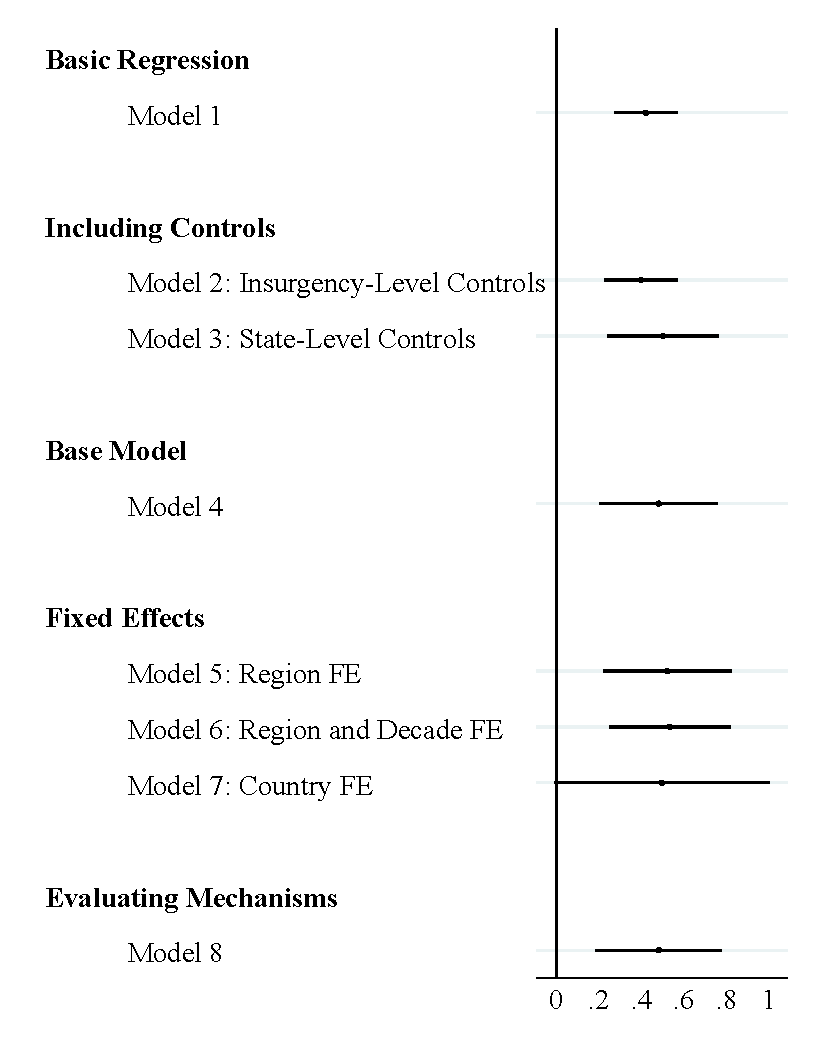
\includegraphics[width=\textwidth]{coefmainint.pdf}
    \end{subfigure}
% 
	\begin{subfigure}{0.45\textwidth}
    \centering
    \caption{\autoref{table:mainintp}} \label{figure:coefpanelint}
    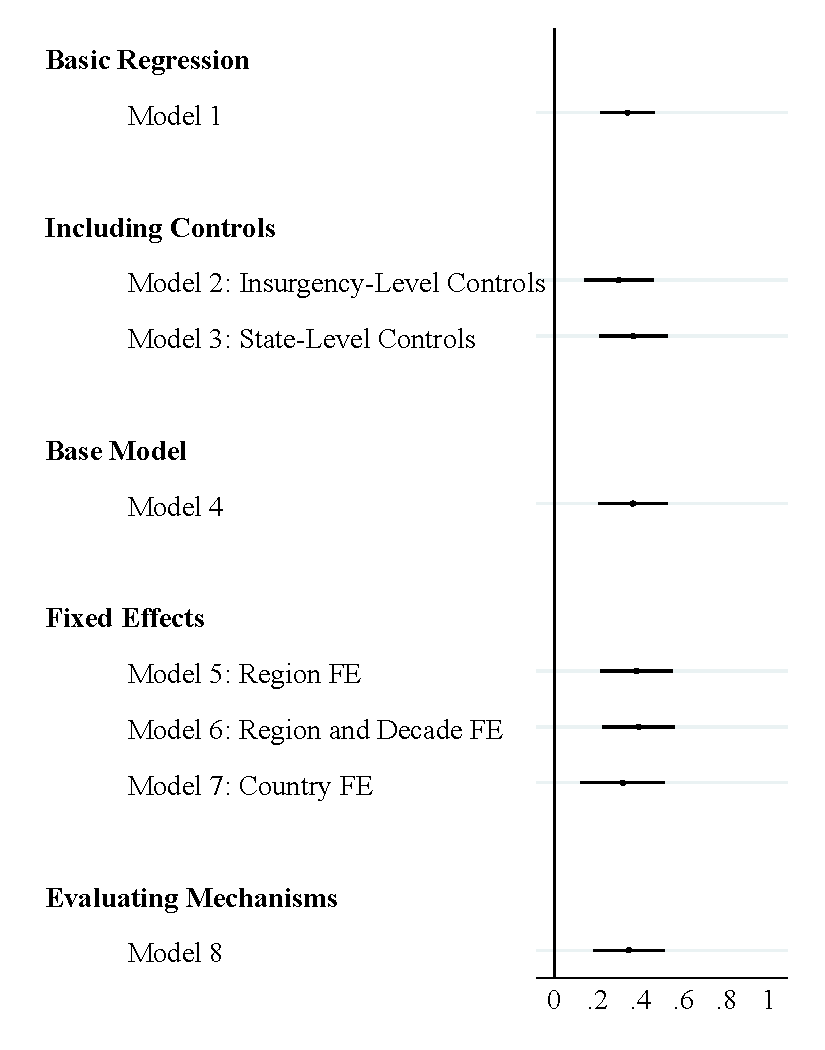
\includegraphics[width=\textwidth]{coefpanelint.pdf}
    \end{subfigure}
  \begin{tablenotes}[para, flushleft]
\raggedright \footnotesize{\textit{Note:} \autoref{figure:coefcomp2} presents the coefficient estimates for the variable \textit{Secessionist  $\times$ Territorial Control} in \autoref{table:mainint} and \autoref{table:mainintp}. Black horizontal lines represent 90\% confidence intervals. If the confidence intervals fail to overlap with the vertical black line, then the effect of \textit{Secessionist} is statistically significant. The estimated effects using these two sets of data are highly similar in terms of statistical and substantive significance.}
\end{tablenotes}
\end{figure}


\newpage
\clearpage
\thispagestyle{plain}
\begin{center}
\Large{\textbf{Appendix 6: Additional Information on the Insurgent Social Service Provision Dataset}}
\end{center}

\normalsize

In this section, I provide a more detailed and extensive overview of the theoretical framework I developed for determining inclusive versus exclusive service provision, the sources I used to code these data, and some of the challenges that I faced. I then explain why I focused on education and healthcare provision specifically and provide definitions for how I operationalized and coded these measures. I go on to present a set of textual examples that I used to code the dataset. These examples demonstrate how I was able to determine not only whether a rebel group provided education and healthcare but also who benefited from rebels' services. Finally, I conclude with a descriptive overview of the dataset, as well as a graphical presentation of trends in provision over time.

\subsection*{A Spectrum of Support for Rebels}  

Support for an insurgency can be conceived as a spectrum of commitment to the insurgency and its goals, with certain civilian groups more or less likely to support and/or join the rebel group. On one hand of this spectrum are active rebel combatants, with never-joiners (such as members of the incumbent regime) on the other end of this spectrum. The majority of the population falls in between these categories. Within this broad center, civilians may be classified as already active supporters of the rebel group with weaker commitments, as neutral civilians with no commitments but who may be otherwise inclined to support and join the insurgency because of the rebel group's political platform, or finally as unlikely supporters and joiners who do not represent an insurgency's core constituency or political community.\footnote{\citealt{stewart2015good}} This spectrum of support is highly similar to how some military officials conceive of popular support in insurgency and counterinsurgency operations, suggesting that this conception of support has useful theoretical and empirical applications.\footnote{\citealt[71-2]{packwood2009popular}} Figure \ref{figure:spectrumgen} below presents this spectrum graphically. 
 
\begin{figure}[h!]
\centering
\begin{center}
\renewcommand\thefigure{A.\arabic{figure}}
\caption{\textbf{A Spectrum of Support for Insurgencies}}
\label{figure:spectrumgen}
\scalebox{.45}{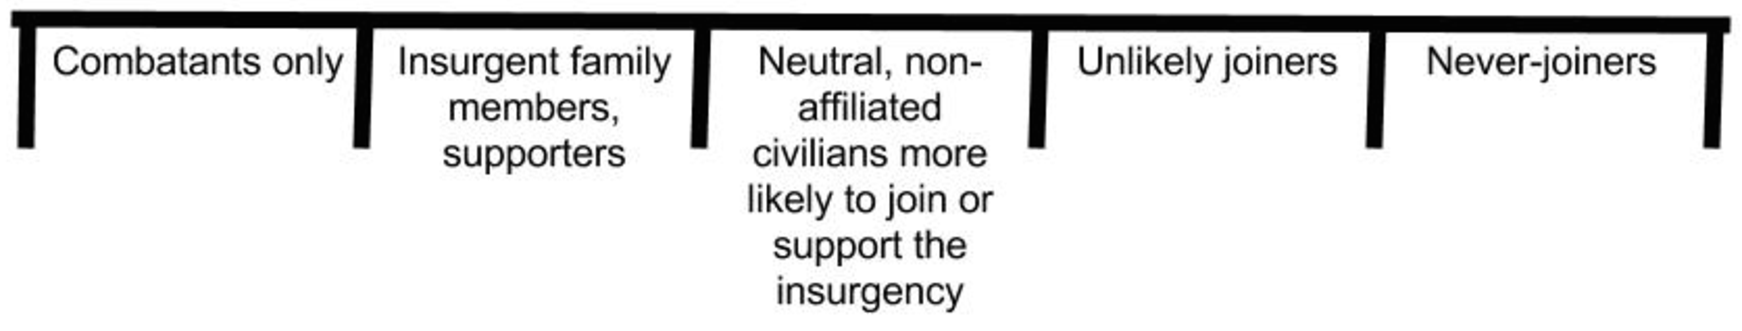
\includegraphics{spectrumgeneral.pdf}}
\end{center}
\end{figure}

The spectrum outlined above, however, is a theoretical construct. In Figure \ref{figure:spectrumspecific}  below, I delineate the observable implications of each of these theoretical categories. I consider neutral non-joining civilians as people who the rebel group explicitly seeks support from and are core members of the insurgency's coalition. For communists, these tend to be peasants, and in some cases, workers. On the other hand, unlikely joiners or supporters would include wealthier merchants or businesspeople, clergy members or traditional leaders, intellectuals or the bourgeoisie. For secessionist or ethnic insurgencies, neutral but likely joiners tend to be co-ethnics, co-religionists or co-linguists. People not of the insurgency's predominant ethnicity, religion or linguistic group represent unlikely joiners. For any rebel group, former supporters of a different insurgency can be classified as unlikely supporters, as would prisoners of war that a rebel group has captured. For some Islamist groups, such as the Taliban, women are unlikely supporters and joiners. 

\begin{figure}[h!]
\centering
\begin{center}
\renewcommand\thefigure{A.\arabic{figure}}
\caption{\textbf{Observable Implications of a Spectrum of Support}}
\label{figure:spectrumspecific}
\scalebox{.45}{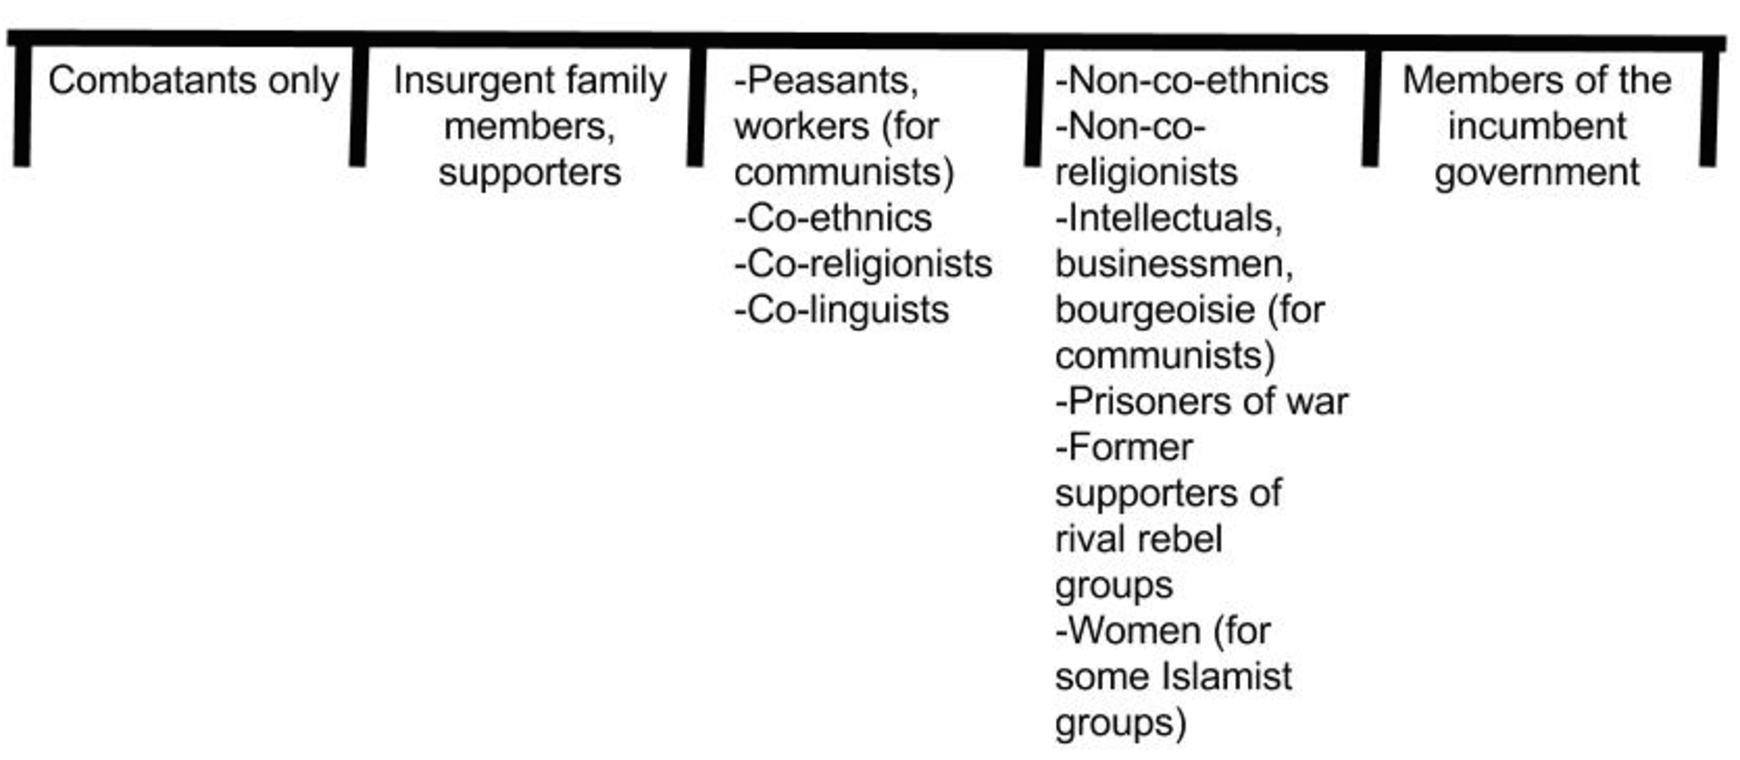
\includegraphics{spectrumspecific.pdf}}
\end{center}
\end{figure}

Using these distinctions, I code as inclusive service provision any rebel group that provided to unlikely joiners or never joiners. I code as exclusive service provision any insurgency whereby the organization provided only to members of the insurgency, to members of the insurgency and active supporters, or to neutral civilians who may be more likely to join the rebel group (Figure \ref{figure:coding}). Although these data represent an attempt to systematically and verifiably code the extensiveness and inclusivity of rebel governance, this measure is imperfect and cannot accurately predict each individual person's likelihood to be recruited by a rebel group. There may be idiosyncratic reasons why a person who is an unlikely joiner becomes a member of a rebel group. However, on average, the intuition that non-co-ethnics are less likely than co-ethnics to join an ethnic or secessionist insurgency is mostly true. In the same way, peasants are probably more likely to join a communist insurgency than wealthy merchants, on average.

\begin{figure}[h!]
\centering
\begin{center}
\renewcommand\thefigure{A.\arabic{figure}}
\caption{\textbf{Operationalizing Inclusive Provision}}
\label{figure:coding}
\scalebox{.45}{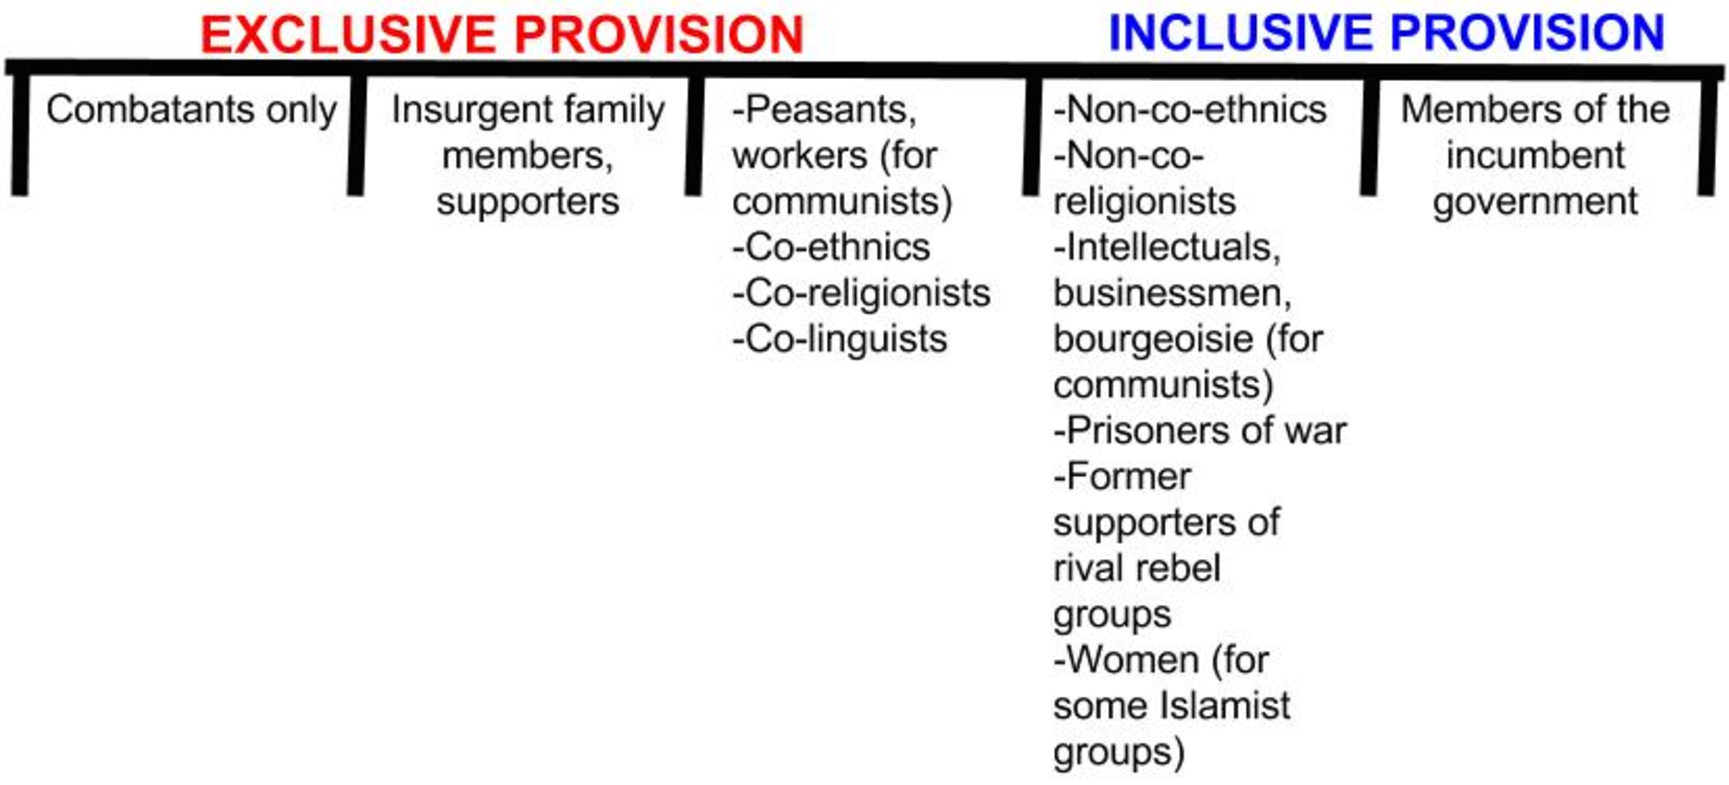
\includegraphics{coding.pdf}}
\end{center}
\end{figure}

It is worth noting that inclusive and exclusive service provision are not mutually exclusive. Even when providing inclusive services, insurgencies can also provide exclusive services simultaneously. In these cases, rebels provide services in tiers. More active and dedicated supporters receive higher quality education or training, including being sent abroad to study. Unlikely joiners receive basic literacy classes and rudimentary healthcare, but receive education and healthcare nonetheless. Therefore, the provision of inclusive services is not an indication that the insurgency prefers unlikely supporters over loyal members. An example of this tiered system is the African Party for the Independence of Guinea and Cape Verde (PAIGC), whose education services are described as ``literacy for all, quality education for some.''\footnote{\citealt[97]{dhada1993warriors}} For its strongest and most committed adherents, the PAIGC offered high quality education in the capital Conarky or offered scholarships to study abroad. For everyone else, the PAIGC provided minimal public schooling throughout the country.\footnote{\citealt[106-7]{dhada1993warriors}} In these lower quality facilities, the PAIGC provided basic education and literacy courses, but little more. In other words, although a rebel group provided inclusive services, this by no means implies that it privileged unlikely joiners over committed followers. Rather, it underscores the theoretical logic presented in the manuscript: insurgencies could provide high quality, exclusive services for recruitment and retention purposes, and yet rebels could still also provide services to the population writ large, including unlikely supporters. Why rebels go beyond the initial high quality education services reserved for followers is what drives my research and what I aim to address in this manuscript.

\subsection*{Service Provision Over Time}  

These data are time-variant and capture changes in when rebel organizations began providing services or stopped. In most cases, specific dates for when services were provided was available in the text. Other times, texts would say that ``by a given year'' or ``in the mid-1980s'' (for example), a rebel group would have established social service institutions. In these cases, all years before that particular period of time are coded as missing. Additionally, some rebel groups also changed their level of provision. This typically occurred after an insurgency controlled territory: for example a rebel group might have only provided education and health to its cadres until the organization captured territory. Once the insurgency controlled territory, the rebel group might have started to provide services more broadly to civilians living in the territory it captured. In some rare cases, such as the People's Liberation Army (PLA) in China in 1948, or Hezbollah after 1991, education moved from neutral supporters to more inclusive provision of unlikely joiners (both cases are discussed more in the main text).

\subsection*{Sources}  

To code these data, I relied primarily on secondary literature, especially secondary case histories on each rebel group. I also relied on newspaper and magazine articles collected through Lexis Nexis or Google web searches, journal articles, archival documents, testimonies, reports and memoirs. Because I code service provision in refugee camps, some NGOs such as Amnesty International or INGOs such as the United Nations had rich data on the governance of these refugee camps. Feminist accounts of the rebellion tended to have the best data: women were often asked to perform these service-providing roles and would detail the inclusivity and extent of rebel service provision. For an example of four different sources I used (newspapers, websites about refugee camps and case histories) please see the section below on examples of the coding procedure (pp. 57).  

To the best of my abilities, I triangulated my coding with as many sources as possible. These sources were mostly written in English, but I did use other sources written in Spanish and French. These language choices mirror those selected by Shapiro.\footnote{\citealt{shapiro2013terrorist}} The data coding process took place between October 2013 and October 2014, and research assistants served to validate the coding procedures as well. 

\subsection*{Missingness and Coding Challenges}  
Some observations are missing, and this typically occurred if a text said the rebel group established ``services'' but never specified which, or if the insurgency set up a health or education ministry, but no further information about whether the group actually enacted any service provision could be found. As I note below, the Nationalist Socialist Council of Nagaland (NSCN) created an education ministry, but no information about whether this ministry actually offered services could be identified.\footnote{\citealt{satp2014}} 

Because excludability is critical to the research question of this manuscript, observations without information on exclusion are coded as missing in the current analysis. If I found data that the rebel group provided services, but could not find information on exclusion, I coded the \textit{Inclusive Service Provision} variable as missing, and coded that insurgency as providing \textit{any} education or health in a separate variable not used for this analysis. This was the case for five different insurgencies, such as the United Democratic Resistance Movement in the Soviet Union. 

Alternatively, if any observations had unclear provision that could be considered as providing inclusively or exclusively, I created a second, alternative coding and I use this measure as a robustness check (Appendix Table \ref{table:altpg}). This was an issue with two cases: the Popular Front for the Liberation of Oman and the Arab Gulf (PFLOAG) and Hamas, which produced particularly conflicting accounts. 

To test whether missingness systematically biases in favor of my results, I replace all missing values with a ``0'' signifying that missingness should be considered no inclusive provision (Model 3, Appendix \autoref{table:info}). These results are robust, indicating that missingness does not systematically bias in favor of my results. 

Ultimately, these data are likely imperfect, but I anticipate updating these data as new information becomes available. Like most datasets that have undergone multiple iterations, this work represents a first-cut innovation that nevertheless improves our understanding of rebel governance.


\subsection*{Focus on Education and Healthcare Provision}
The dataset focuses on the provision of education and healthcare specifically. I use these services for three reasons. The first is that there is great variation in insurgent services provision, and I needed services that were comparable across time and space. As an example of this variation, insurgencies have provided everything from food aid or ``justice'' to building hydroelectric power plants (Burmese Communist Party).\footnote{\citealt[Appendix II]{lintner1990rise}} Due to the variation in the types of services insurgencies provide, I limit my focus to education and healthcare to ensure that I am comparing similar services across space and time. Education and healthcare are two such services that are comparable across cases and across time. A literacy or mathematics course in the 1970s in Africa will be similar to mathematics or literacy courses in Asia in the 1950s or in Latin America in the 1980s. Similarly, because what is generally healthy for one person is likely also going to be beneficial for another person anywhere else in the world or at any other time since 1945, healthcare is broadly similar across space and time. 

The second reason I focus on these two services is that education and healthcare are broadly desirable to all people and are services from which all people can benefit. As a result, exclusion from education or healthcare institutions clearly demonstrates the populations to which the insurgency is or is not providing social services. For example, insurgencies such as the Front for the National Liberation of Congo (FNLC) may provide food to the starving or most impoverished.\footnote{\citealt{moroccan1977, wright1977katanga}} Yet, because the majority of people are not starving or impoverished, they may be ineligible to receive these services at any given point. Because the social services data I collected also takes into account who can benefit from services, I do not examine any services that people might be ineligible to receive, however reasonable their exclusion. If an insurgency offered food to some civilians, and not others, it would be difficult to determine if the insurgency were limiting its provision to only those with economic need, or if the insurgency limited its provision to people with economic need and to people who were also likely to support the insurgency. Therefore, I do not include in my analysis any social service that might exclude members of the population, however reasonably, to ensure the greatest accuracy possible. Education and healthcare do not suffer from this exclusion problem, as ostensibly anyone at any time could benefit from education or healthcare. 

Finally, all people have a reasonable expectation of receiving, either freely or in a deeply subsidized form, education or healthcare. Education and healthcare are codified as essential human rights in the Universal Declaration of Human Rights. In the vast majority of countries, education is constitutionally guaranteed and guaranteed to be free.\footnote{\citealt{worldpolicy}} Almost all countries have free or compulsory education.\footnote{\citealt[32-80]{tom2001}} Although healthcare is sometimes more complicated (particularly in countries like the United States), governments in almost all countries still allocate resources to subsidize and supplement healthcare throughout their state.\footnote{\citealt{worldbankhealth}} Although these services are not always considered classic state-provided public goods like national security or justice, people have a reasonable expectation of receiving these services from the state with little to no cost to themselves.  

\subsection*{Defining Key Terms}
Below, I delineate how I defined ``provision,'' ``education'' and ``healthcare'' while coding.
\\
\\
\noindent \underline{Provision:}
I code insurgencies as ``providing'' services if they diverted their personnel and financial resources to ensure that a certain group of people received education and healthcare. This typically manifests in two ways:
\begin{enumerate}
\singlespacing
\item Insurgencies offered education or healthcare themselves through their construction of schools, development of curriculum, service as teachers and doctors, or building of hospitals as needed.
\item Insurgencies ensured that services continued to operate in the area they controlled, typically through the administration and financing of these services, although these institutions already existed.
\end{enumerate}
I do not code groups as providing services if they allow an NGO, religious group, or the incumbent government to provide services in the areas they control, but the insurgencies themselves did not contribute to this provision. For example, the Liberation Tamil Tigers of Eelam (LTTE) allowed the Sri Lankan government to continue its healthcare provision in the areas the LTTE controlled. The LTTE taxed this service, but was not involved in the direct administration of it. As a result, I do not consider the LTTE to have provided healthcare services.\footnote{\citealt[118-9]{mampilly2011rebel}}
\\
\\
\noindent \underline{Education:}
In the context of a civil war, insurgents or authors of secondary source texts could use the term ``education'' ambiguously, and may refer to propaganda campaigns or general military training as education. If the insurgent organization itself or the secondary literature refers to an insurgency as ``training'' recruits or supporters, and not educating them, I do not consider this to be education. If what the insurgency is providing is not described as training, then I code education as the instruction of skills that can be applied outside of the context of the military operations, such as language, mathematics, or history. If these skills are applicable to both the insurgents' military goals as well as useful outside the context of the insurgency, such as teaching mathematics so that insurgents know how many explosives to use and how to budget resources, I still code this as education. A clear example of education provision is exemplified by the following passage: Hezbollah's ``Educational Center of the Martyr Bojeii opened in 1992 in the village of Mashghara\ldots [I]t has nineteen sections covering both nursery and elementary classes and also serves the children of seven neighboring villages.''\footnote{\citealt[164]{jaber1997hezbollah}} On the other hand, the Nationalist Socialist Council of Nagaland (NSCN) has an education ministry in their structure, but no texts referred to their explicit provision of education to insurgent members or civilians.\footnote{\citealt{satp2014}} From this information above, it is not clear if the NSCN education ministry developed education policy, created propaganda campaigns or actually provided education to others. As a result of this ambiguity, I code this entry as missing. 
\\
\\
\noindent \underline{Health Care:}
I code an insurgency as providing healthcare if the insurgency offered medical treatment. Because of the influence of Mao and China's sponsorship of liberation movements in the Middle East and Africa, some insurgencies provided acupuncture to the populations under its control. Even if an insurgency provided acupuncture, such as the Ethiopian People's Revolutionary Party (EPRP), I consider the group to provide healthcare.\footnote{\citealt[368-9]{tadesse1998generation}} This is to avoid a bias in coding medical care as only ``Western'' medical practices. 


\subsection*{Examples of Coding}
To demonstrate more clearly how these data were coded, I present examples of exclusive or inclusive provision. For rebels that provided exclusive services, I rely on the Sandinista National Liberation Front (FSLN), Zimbabwe's African People's Union (ZAPU), and the case of Ethiopian People's Revolutionary Party (EPRP). For insurgencies that provided to unlikely joiners (inclusive services), I present the case of the Eritrean People's Liberation Front (EPLF).

\begin{enumerate}
\item \textbf{Exclusive provision to only combatants: The Sandinista National Liberation Front (FSLN).} The evidence I found for the FSLN supports the idea that the guerrillas only provided education within their own camps. The text below is an excerpt from a newspaper report. A journalist from the \textit{St. Petersburg Times} visited a Sandinista hideaway. There, guerrillas had classes and learned basic mathematics, albeit for the purpose of learning how to calculate the appropriate amount of explosives to use in certain situations. From the report: 
\begin{quote}
``Our reporter was taken to the camp by Eden Pastora, the famous ``Commander Zero'' of last summer's attack on the National Palace in Managau \ldots The guerrillas are almost all young. Many are seasoned combat veterans by the time they reach age 20. \ldots The guerrillas sleep in an area that doubles as a classroom during daylight hours. The day begins at 4:45am \ldots The Commandos train in the field until the afternoon rains arrive, and they take cover for weapons instruction. \textbf{Men who have never mastered simple mathematics are trained to compute such essential calculations such as the proper charge to blow up a bridge, or a tree, or a house.} The training does not end at nightfall. Squads of men hold political meetings to discuss the principles for which they are fighting.''
\end{quote} 
As the quote demonstrates, guerrillas living in the camps in 1978 were learning mathematics, albeit for military purposes, but nonetheless received some education. This supports my coding of the FSLN as providing exclusive services to only combatants in 1978. Because no other texts mention the FSLN providing services outside its core guerrilla camp, we can be reasonably confident that education was primarily restricted to group members. 
\item \textbf{Exclusive provision to only supporters and combatants: Zimbabwe's African People's Union (ZAPU).} The case of ZAPU represents an insurgency that provided services to supporters and members. ZAPU provided these services within a refugee camp, the only place they were able to hold territory.\footnote{\citealt{cunningham2009takes}} During the war, ``the Rhodesian regime retaliated ever more viciously and the civilians became the victims. The majority supported the guerrillas'' and they fled across the borders where they became ``ZAPU refugees'' primarily in one of two refugee camps: Victory Camp and JZ Moyo Camp.\footnote{\citealt{zapuweb}} Though the camp was poorly equipped initially, ``ZAPU did eventually have good medical provision for the refugees in the camps and did make an effort to avoid those problems which might be caused by poor sanitation or poor hygiene.''\footnote{\citealt{zapuweb}} ZAPU did not control territory outside of the refugee camp, and no other textual evidence indicated more extensive or inclusive provision elsewhere. As is clear from the text, ZAPU supporters fled to the refugee camp and became ``ZAPU refugees.'' Because ZAPU only provided to supporters and members, its services are exclusive.
\item \textbf{Exclusive provision to neutral civilians: The Ethiopian People's Revolutionary Front (EPRP).} The EPRP was a communist group. Therefore, the EPRP's primary political base, the people most likely to support the EPRP's political platform and the people most likely to be targeted for recruitment were rural peasants. For peasants lacking any education, the EPRP conducted literacy campaigns while more advanced recruits ``conducted political discussion sessions on a regular basis and departments prepared reading materials.''\footnote{\citealt[366]{tadesse1998generation}} In addition, the EPRP ``had its own clinic where members and peasants were treated. The clinics were staffed by medical doctors, pharmacists, qualified health officers and nurses.''\footnote{\citealt[368]{tadesse1998generation}} One of the common treatments the EPRP administered to both its members as well as civilians was acupuncture. Acupuncture was ``introduced by [EPRP] members who had been trained by Chinese medical groups in South Yemen who in turn trained others.''\footnote{\citealt[368]{tadesse1998generation}} The EPRP gained considerable popularity among the peasantry because of its acupuncture treatments and their seeming effectiveness. Moreover, the EPRP in the western part of the Begemidir province of Ethiopia also established abortion clinics.\footnote{\citealt[369]{tadesse1998generation}} The text here demonstrates that the EPRP provided services to neutral civilians and members, making the distinction in the text between ``members'' and ``peasants.'' The text itself was written by a member of the EPRP as well, and thus had inside knowledge of the EPRP's behavior. More inclusive provision was not mentioned in any other texts by the EPRP, and thus we can be assured that the EPRP's provision though extensive, was nonetheless exclusive.
\item \textbf{Inclusive provision to unlikely joiners: The Eritrean People's Liberation Front (EPLF).} Eritrea has nine different ethnicities and two major religions (Islam and Christianity). Ethnicities tended to fall along religious lines. The EPLF was primarily a Christian organization and drew many of its core supporters from co-religionists. The EPLF also fought against the rival secessionist organization, the Eritrean Liberation Front (ELF). The ELF was primarily Muslim. Therefore, Muslims would be unlikely supporters. Moreover, the EPLF was a communist organization, so conservative, wealthier merchants and businesspeople were also unlikely supporters. Finally people living in towns previously controlled by the ELF or people who were ELF supporters would be unlikely to join or support the EPLF. Pool\footnote{\citealt{pool2001guerrillas}} provides an overview of the EPLF's 1977 conquest of a town in Eritrea called Keren. Keren was very conservative, wealthy and had a larger Muslim population. Additionally, the ELF, the main rival of the EPLF, had previously maintained a significant presence and support there,\footnote{\citealt[121]{pool2001guerrillas}} and the ELF propaganda had led some of the local population to nickname the EPLF the ``Eritrean Derg.''\footnote{\citealt[123]{pool2001guerrillas}} As a result, Keren ``was a more difficult proposition'' for liberation by the EPLF than other towns.\footnote{\citealt[123]{pool2001guerrillas}} Despite these challenges, the EPLF proceeded with liberation and reconstruction, and implemented a series of wage reforms, price controls, taxes and education and healthcare initiatives that became very popular. One member of the town:
\begin{quote}
``[S]tate[d] that even the bourgeoisie was pleased with liberation. They had expected the EPLF to be like the Derg, but it was not because their property and riches were preserved. The EPLF placed great stress on the provision of services. Keren hospital, badly damaged during the fighting, was repaired and reopened. An EPLF clinic with an EPLF doctor was attached to the hospital and medical supplies were brought from the central pharmacy. Increasingly, rural people with serious conditions were referred to Keren hospital by squad doctors operating in the surrounding areas. Schools were reopened and continued to function despite the fact that teachers' salaries were not coming through from Asmara [the Ethiopian-controlled capital of Eritrea]. The EPLF succeeded to the array of local taxes and levies collected by the Ethiopian government: rent from nationalized properties, charges for veterinary checks on animals brought for sale in the market, for example. Ethiopian taxes were diverted for the provision of goods and services.''\footnote{\citealt[124-5]{pool2001guerrillas}}
\end{quote}
The quote above demonstrates that the EPLF provided services to unlikely supporters or joiners of the rebel group, and this was a systematic approach to governance. In addition to providing to unlikely joiners, the EPLF also provided education and healthcare to \textit{Ethiopian} prisoners of war.\footnote{\citealt[91]{wilson1991challenge}} Because these soldiers were Ethiopian and would never benefit from the Eritrean after the war, this is another indication of provision to people unlikely to support the rebel group.
\end{enumerate} 


\subsection*{External Validation and False Positives}
I turn to two existing datasets to externally validate the coding results, to address concerns of bias in coding arising from the hand-collected nature of the dataset. If the data I collected correspond to these existing datasets well, then confidence in my coding procedures should be improved. Nation-states are the traditional providers of inclusive services, especially healthcare and education. One may anticipate that insurgencies that provide inclusive goods behave as if they are states. Thus, insurgencies that provide inclusive goods may appear in the De Facto States in International Politics (1945-2011) Dataset.\footnote{\citealt{florea2014facto}} Florea\footnote{\citealt[5-6]{florea2014facto}} lists 34 de facto states and of these, 21 are also included in the NSA Dataset as either insurgencies or the de facto states that are products of insurgencies.\footnote{For example the Karen National Union in the NSA Dataset created what Florea calls ``the Karen State,'' and what the Karens call ``Kawthoolei.''} Among this group of 21 de facto states, over 80\% are coded as providing inclusive goods (16 groups). Furthermore, Kalyvas and Balcells (2010) argue that some civil wars are conventional civil wars where ``military confrontation is direct, either across well-defined front-lines or between armed columns.''\footnote{\citealt[419]{kalyvas2010international}} One would predict that insurgencies that provide inclusive services could be acting as if they were states, and thus engage in conventional warfare as states do. Of the 46 conventional wars, insurgencies provided inclusive services in 15 of these.\footnote{\citealt{kalyvas2010international}} The correlation between these two datasets and the \textit{Inclusive Service Provision} variable offers external support for the reliability of the data. 

These data are also highly responsive to instances that appear to be inclusive provision when rebel groups in fact exclude certain constituencies from the insurgencies' services. These occurrences are most likely to arise in two ways. First, an insurgency may provide services to anyone within a town or territory it controlled, but only after expelling or killing anyone outside the insurgency's core political constituency. These insurgencies are coded as providing exclusive services. Second, when civilians move to refugee camps during wartime, they may choose from several different locations. People who support the insurgency might move to the camp that an insurgent group controls, while people who support the government may move to camps the government controls. As a result, when the insurgency provides social services in the refugee camp, it appears that the insurgency is providing to everyone when it really provides to supporters, creating a false-positive. To address this issue, I examine the demographics of the refugee camp. If the refugee camp population contains more than 90\% of people who are likely to support the insurgency (co-ethnics, co-religionists, etc.), I do not code this group as providing inclusive services. 

\subsection*{Descriptive Overview of Insurgent Social Services Dataset}

The Insurgent Social Services Dataset contains 313 unique rebel groups. Of these, 104 insurgent groups provided some form of education, or approximately 33\% of rebel groups provided any education between 1945 and 2003. Nearly 49\%, or 154 groups, provided no education, and 55 groups have missing observations (18\%). %Of the total observations, 894 insurgency-years experience education provision, meaning that 37\% of all insurgency-years included education provision. \footnote{Some of these cases are somewhat challenging to code because many had considerable autonomy, if not outright independence before the civil conflict began. These states tend to be former Soviet (Nagorno-Karbagh, South Ossetia) or Yugoslav (Croatia, Serbia, etc.)  states, or states that were occupied by the Japanese in World War II, granted independence when the Japanese knew they were losing, then were retaken as colonies by victorious European states. This group of cases with considerable autonomy includes: Autonomous Province of Western Bosnia, Croatian Republic of Bosnia and Herzegovenia, Dniestr Republic, Independent Mining State of South Kasai, Indonesian People's Army, Katanga, Lao Issara,  Palestine National Authority (PNA),  Popular Front, Republic of Abkhazia, Republic of Biafra, Republic of Chechnya, Republic of Dagestan, Republic of Nagorno-Karabakh, Republic of South Moluccas, Republic of South Ossetia, Serbian Republic of Bosnia and Herzegovenia, and the Serbian Republic of Krajina.}

Correspondingly, approximately 102 groups provided healthcare, meaning that about 33\% of insurgencies provided healthcare, while 148 insurgencies provided nothing, or 45\%. For 63 groups, or  21\% of insurgencies, the data are missing. %Approximately 33\% of all observations experience healthcare provision, or about 794 insurgency-years.  

Most insurgencies either provided no education and no healthcare, or provided both education and healthcare. Just 7\% of insurgencies provided healthcare but not education, and just 5\% of insurgencies provided just education but not healthcare. About 95\% of groups that provided education inclusively also provided and healthcare inclusively. 

\newpage
\begin{center}
\begin{figure}[h!]
\renewcommand\thefigure{A.\arabic{figure}}
\begin{center}
\caption{\textbf{Annual Total Insurgent Education Provision, Globally 1945-2003}}
\label{figure:insurgenteduany}
\scalebox{1}{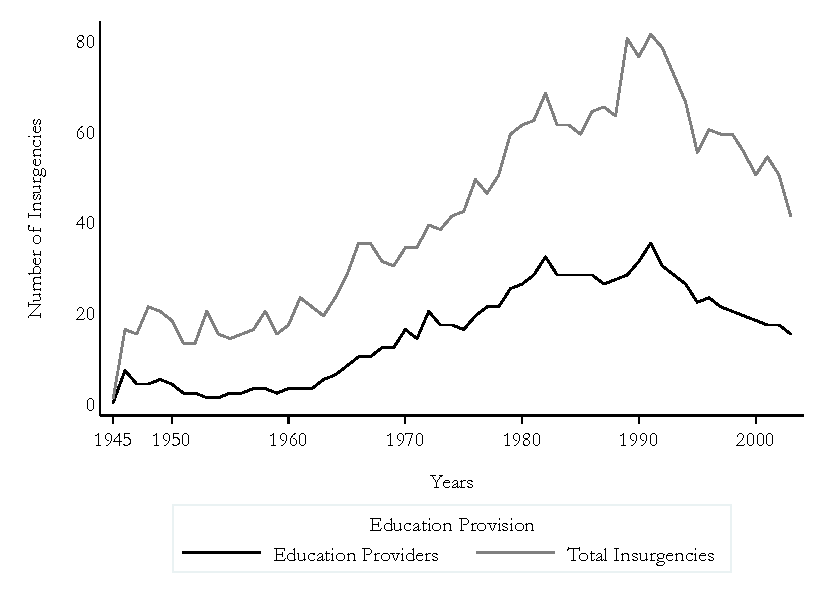
\includegraphics{insurgenteduany.pdf}}
\end{center}
\begin{tablenotes}[para, flushleft]
\raggedright \footnotesize{\textit{Note:} The figure demonstrates the number of insurgencies providing education globally from 1945-2003.} 
\end{tablenotes}
\end{figure}
\end{center}

\newpage
\clearpage
\begin{center}
\begin{figure}[h!]
\renewcommand\thefigure{A.\arabic{figure}}
\begin{center}
\caption{\textbf{Annual Insurgent Education Provision, Globally 1945-2003}}
\label{insurgenteduannual}
\scalebox{1}{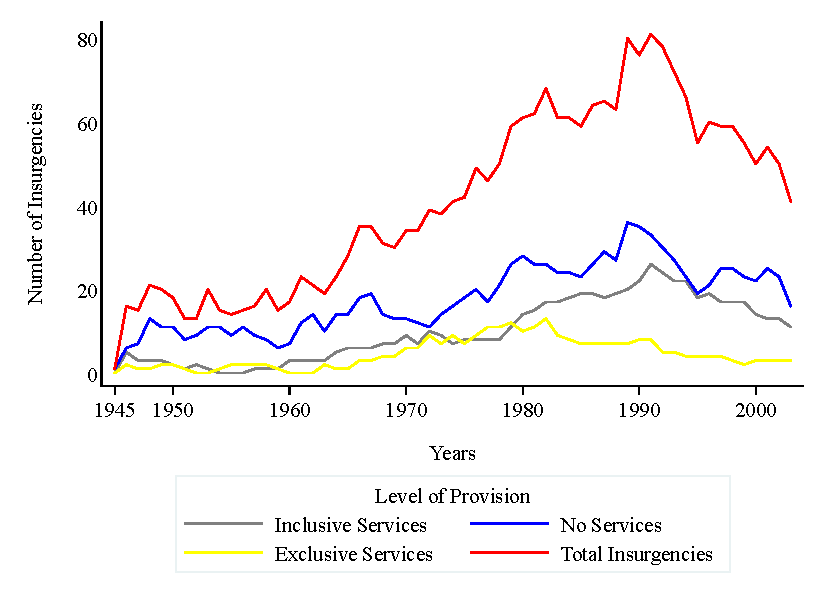
\includegraphics{incexedu.pdf}}
\end{center}
\begin{tablenotes}[para, flushleft]
\raggedright \footnotesize{\textit{Note:} \footnotesize The figure demonstrates the annual level of insurgent education provision globally from 1945-2003.} 
\end{tablenotes}
\end{figure}
\end{center}


\newpage
\begin{center}
\begin{figure}[h!]
\renewcommand\thefigure{A.\arabic{figure}}
\begin{center}
\caption{\textbf{Annual Total Insurgent Healthcare Provision, Globally 1945-2003}}
\label{insurgenthealthany}
\renewcommand\thefigure{\Roman{figure}}
\scalebox{1}{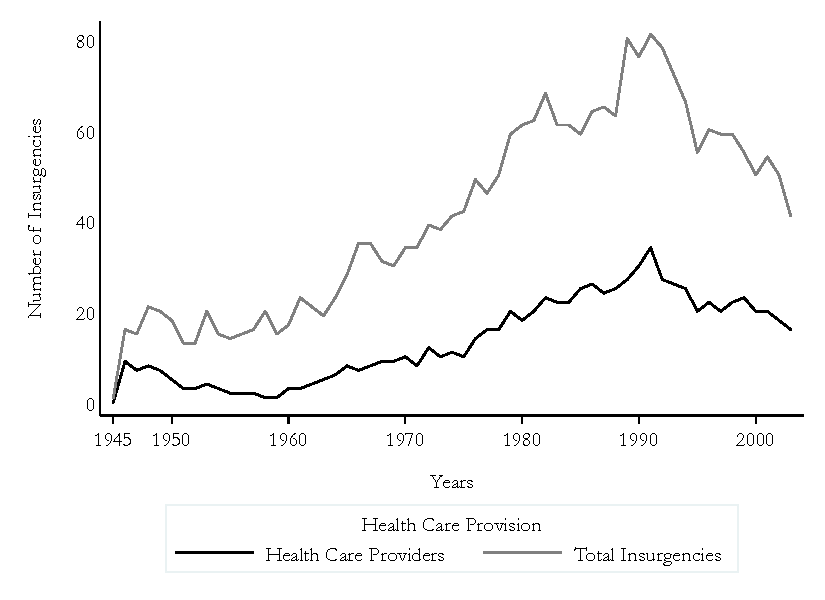
\includegraphics{insurgenthealthany.pdf}}
\end{center}
\begin{tablenotes}[para, flushleft]
\raggedright \footnotesize{\textit{Note:} \footnotesize The figure demonstrates the number of insurgencies providing healthcare globally from 1945-2003.} 
\end{tablenotes}
\end{figure}
\end{center}


\newpage
\begin{center}
\begin{figure}[h!]
\renewcommand\thefigure{A.\arabic{figure}}
\begin{center}
\caption{\textbf{Annual Insurgent Healthcare Provision, Globally 1945-2003}}
\label{figure:insurgenthealthannual}
\scalebox{1}{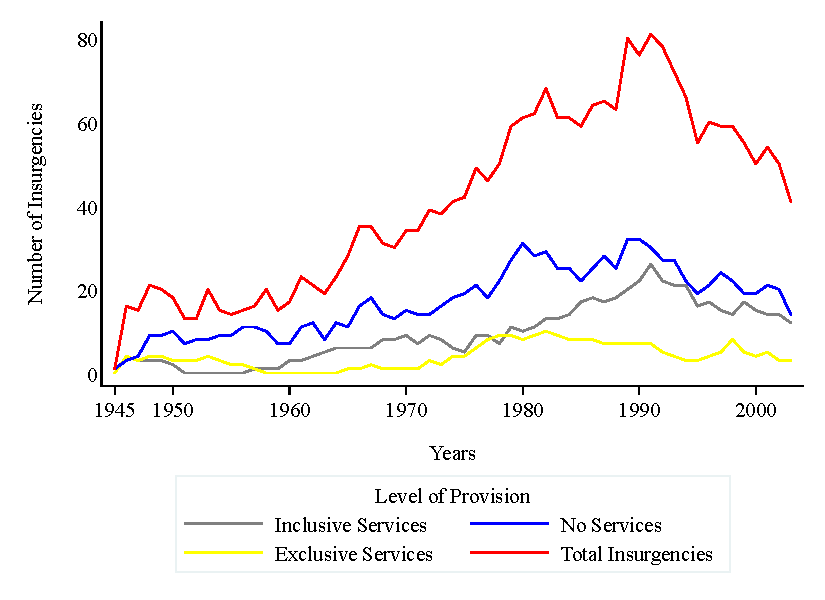
\includegraphics{incexhealth.pdf}}
\end{center}
\begin{tablenotes}[para, flushleft]
\raggedright \footnotesize{\textit{Note:} \footnotesize The figure demonstrates the annual level of insurgent healthcare provision globally from 1945-2003.} 
\end{tablenotes}
\end{figure}
\end{center}

%\newpage 
%\begin{center}
%\begin{figure}[h!]
%\renewcommand\thefigure{A.\arabic{figure}}
%\begin{center}
%\caption{\textbf{Insurgent Inclusive Education and Healthcare, By Region}}
%\label{graphregion}
%\scalebox{1}{\includegraphics{graphregion.pdf}}
%\end{center}
%\begin{tablenotes}[para, flushleft]
%\raggedright \footnotesize{\textit{Note:} The figure demonstrates the number of insurgencies providing inclusive and those not providing inclusive services by region. The y-axis indicates the percent of insurgencies in a region providing inclusive services or not. The values on top of each bar indicate the total number of groups providing inclusive services or not. Missing observations are excluded.}
%\end{tablenotes}
%\end{figure}
%\end{center}



%===================References=====================




\end{document}